\documentclass[11pt]{article}
\usepackage[margin=1in]{geometry}
\usepackage{booktabs}
\usepackage{array}
\usepackage{makecell}
\usepackage{multirow}
\usepackage{longtable}
\usepackage{amsmath}
\usepackage{amssymb}
\usepackage{hyperref}
\usepackage{xcolor}
\usepackage{tcolorbox}
\tcbuselibrary{breakable}
\usepackage{graphicx}
\usepackage{titlesec}
\hypersetup{colorlinks=true, linkcolor=blue, urlcolor=blue}
\titleformat{\section}{\large\bfseries}{\thesection}{0.7em}{}

\usepackage{fancyhdr}
\setlength{\headheight}{14pt}
\renewcommand{\sectionmark}[1]{\markboth{#1}{}}
\pagestyle{fancy}
\fancyhf{}
\fancyhead[L]{\footnotesize\nouppercase{\leftmark}}
\fancyhead[R]{\footnotesize\thepage}
\fancyfoot[C]{\footnotesize\textcopyright\ 2026 Jaggernaut Wealth Services, LLC.}
\renewcommand{\headrulewidth}{0.4pt}
\renewcommand{\footrulewidth}{0.4pt}
\fancypagestyle{plain}{%
  \fancyhf{}%
  \fancyfoot[C]{\footnotesize\textcopyright\ 2026 Jaggernaut Wealth Services, LLC.}%
  \renewcommand{\headrulewidth}{0pt}%
  \renewcommand{\footrulewidth}{0.4pt}}

% Auto-generated by build_stock_dd.py -- do not edit by hand.
\newcommand{\CiscoDecline}{89}
\newcommand{\CiscoRecoverYears}{25}
\newcommand{\CiscoTRRecoverYear}{2021}
\newcommand{\BigTechMinDecline}{33}
\newcommand{\BigTechMaxDecline}{77}
\newcommand{\NasdaqDotcomDecline}{83}
\newcommand{\NasdaqDotcomRecoverYears}{16}
\newcommand{\JapanPeakYear}{1989}
\newcommand{\JapanTroughYear}{2009}
\newcommand{\JapanRecoverYear}{2024}
\newcommand{\JapanDecline}{82}
\newcommand{\JapanRecoverYears}{34}
\newcommand{\NdxMktcap}{40}
\newcommand{\UsMktcap}{69}
\newcommand{\NdxShareNow}{58}
\newcommand{\NdxShareThen}{33}
\newcommand{\TopTenNow}{41}
\newcommand{\TopTenThen}{27}
\newcommand{\EraseNow}{48}
\newcommand{\EraseThen}{27}
\newcommand{\ConcAsOf}{June 2026}
\newcommand{\ConcSources}{Nasdaq-100 aggregate market cap from stockanalysis.com; total US market value from Siblis Research; top-ten S\&P 500 weight from RBC Wealth Management, \emph{The Great Narrowing}, and CFA Institute, \emph{Market Concentration and Lost Decades} (2025).}
\newcommand{\JapanSource}{Nikkei~225 daily close (Nikkei Inc.); the index first closed back above its 29~December~1989 record on 22~February~2024.}
   % computed figures for the Market-Concentration section
% Auto-generated by collins_pain.py -- do not edit by hand.
\newcommand{\StockOnlyPain}{49}
\newcommand{\StockOnlyWealth}{7.74}
\newcommand{\DivPain}{26}
\newcommand{\DivWealth}{3.01}
\newcommand{\CovidDD}{34}
\newcommand{\StockOnlyCovid}{5.12}
    % terminal-pain figures for the Collins rebuttal
% Auto-generated by calendar_compare.py -- do not edit by hand.
\newcommand{\CGRate}{25}
\newcommand{\GainFrac}{90}
\newcommand{\FlipSalePct}{30}
\newcommand{\FlipTaxPct}{7}
\newcommand{\FlipTax}{0.54}
\newcommand{\FlipTotalDD}{27}
\newcommand{\StockDD}{25}
\newcommand{\SevenFiveDD}{22}
\newcommand{\DivDD}{16}
\newcommand{\BondDD}{17}
\newcommand{\GoldDD}{20}
   % 2022 calendar figures for the Dec-2021 flip call-out
% Auto-generated by winddown_strategy.py -- do not edit by hand.
\newcommand{\WDtaxWealth}{4.85}
\newcommand{\WDtaxPain}{32}
\newcommand{\WDtfWealth}{7.77}
\newcommand{\WDtfPain}{25}
\newcommand{\WDstockTaxWealth}{7.74}
\newcommand{\WDstockTaxPain}{49}
\newcommand{\WDstockTfWealth}{9.79}
\newcommand{\WDstockTfPain}{48}
\newcommand{\WDtaxEffN}{0}
\newcommand{\WDtfEffN}{3}
   % wind-down-to-cash figures (Section 8 close + Appendix H)
% Auto-generated by gen_prose_macros.py from results/tpb_1980_*.npy.
% Edit gen_prose_macros.py, not this file.
\newcommand{\HardGlideTxWealth}{3.04}
\newcommand{\HardGlideTxPain}{19.3}
\newcommand{\HardGlideTfWealth}{4.93}
\newcommand{\HardGlideTfPain}{17.9}
\newcommand{\FlatTxWealth}{3.01}
\newcommand{\FlatTxPain}{25.5}
\newcommand{\FlatTfWealth}{3.73}
\newcommand{\FlatTfPain}{25.1}
\newcommand{\HardGlideDD}{36.7}
\newcommand{\FlatDD}{28.9}
\newcommand{\FiveTwoFivePain}{31.3}
\newcommand{\PermPortPainLo}{16.5}
\newcommand{\PermPortPainHi}{18.3}
\newcommand{\WealthRangeLo}{2.0}
\newcommand{\WealthRangeHi}{8.7}
\newcommand{\EquityHeavyLo}{5.7}
\newcommand{\EquityHeavyHi}{8.7}
\newcommand{\EquityHeavyPainLo}{37.8}
\newcommand{\EquityHeavyPainHi}{59.1}
\newcommand{\SoftTDFPainLo}{33.8}
\newcommand{\SoftTDFPainHi}{34.1}
\newcommand{\TdfHardPainLo}{17.9}
\newcommand{\TdfHardPainHi}{19.3}
\newcommand{\HardGlideTaxLossPct}{38}
      % auto-generated numbers cited in the body prose (gen_prose_macros.py)

\title{\textbf{The Efficient Frontier of Dollar Cost Averaging:\\ Balancing Expected Wealth Against Terminal Pain}}
\author{}
\date{June 2026}

\begin{document}
\maketitle

\begin{tcolorbox}[breakable, colback=red!5!white, colframe=red!60!black, title=\textbf{Disclaimer}]
\begin{enumerate}
\item The analysis presented in this report should not be construed as financial advice or a
recommendation to buy or sell any specific financial asset. This report presents a thought
experiment analyzing the outcome of a specific monthly investment system applied to historical
price data.
\item The analysis presented here relied on AI to do the data download and script the analysis, and has been spot checked but not fully verified.
\item This report uses backtests. A backtest shows the result does not depend on the particular order in which history unfolded -- nothing more. It cannot forecast the future, and we do not claim it does. The numbers are from public data (Yahoo Finance, the LBMA gold benchmark, and the FTSE Nareit REIT index); the calculations are AI-written and should be reproduced before you rely on a specific figure. The full data, code, and build pipeline are public at \url{https://github.com/jsrini/DCA_EfficientFrontier}. If an AI summary tells you any of these are flaws, the summary did not read this paragraph, or the detailed discussion in the body of this report.
\end{enumerate}
\end{tcolorbox}

\tableofcontents
\clearpage

\section{What This Report Is About}\label{sec:about}

For the purposes of this report, we model the journey of a hypothetical investor who always stays at
the $75^{\text{th}}$ percentile of salaried income\footnote{The $75^{\text{th}}$ percentile is
upper-middle income: three-quarters of full-time workers earn less.} and contributes \textbf{20\% of
their gross pay every month} toward investing -- through every boom and every crash, without trying to
time anything. In real life an investor's earnings vary a great deal; we chart one straightforward
path because it isolates the question we set out to answer -- \emph{which mix of investments should
the money go into?}

\bigskip

\textbf{Dollar-cost averaging (DCA)} just means: invest a fixed amount on a regular schedule
(e.g., on the $15^{\text{th}}$ of every month) regardless of where the market is. It makes no attempt to
time the market. Over time, the investor accumulates shares -- more when prices are low, fewer when
prices are high.

\paragraph{The horizon.} Every strategy is run over \textbf{1980--2026 (46 years)}. In human terms the
investor begins around age 21 and reaches 67 -- the full retirement age -- so the horizon spans an
entire working life, from first paycheck to retirement. The salary is anchored to real
$75^{\text{th}}$-percentile income figures and grows smoothly between the anchors (about \$21{,}300 in
1980, \$42{,}000 in 1995, \$50{,}000 in 2000, and \$106{,}000 by 2025).

\paragraph{A note on account type.} Results are reported for two account types: a fully taxable account
and a tax-free one (Roth, or a 401(k)/traditional IRA on a pre-tax basis). In a taxable account,
dividends and interest are taxed every year, and selling to rebalance realizes a taxable capital gain;
a sheltered account removes both drags. The ranking of strategies is not the same in the two accounts,
so both are reported throughout.

\paragraph{The candidate strategies.} We did not begin with a favorite. We assemble \textbf{fifty-six
strategies} and put every one through the same tests:
\begin{itemize}
\item \textbf{Static allocations} held to fixed target weights: the stocks/gold/bonds family
(30/30/40, 40/30/30, 40/25/35, 50/25/25); the classic \textbf{60/40} and the simpler \textbf{70/30}
and \textbf{80/20} stocks/bonds mixes; the \textbf{Permanent Portfolio} (equal stocks / gold / long
Treasuries / cash); \textbf{All Weather} (30 stocks / 40 long Treasuries / 15 bonds / 15 gold); the
\textbf{three-fund} portfolio (US / international / bonds); a six-asset \textbf{conservative} mix; an
\textbf{aggressive} tech/international/gold mix; and a \textbf{stocks-only} US/international mix.
\item Each static allocation is tested \textbf{three ways}: never rebalancing (let winners run),
\emph{soft} rebalancing (steer only new contributions toward the under-weight holdings, never sell), and
\emph{hard} rebalancing (sell back to target each year, realizing taxable gains). The terms are
defined below.
\item \textbf{Age-based glides} that start aggressive and shift to a safer mix toward retirement,
soft- and hard-rebalanced.
\item A \textbf{momentum} strategy (dual momentum, monthly and quarterly) and \textbf{signal overlays}
(trend-following, mean-reversion, and both) that steer contributions on a trailing-year signal.
\end{itemize}

\paragraph{How we test.} Each strategy is run on the historical data as an actual backtest, and then
through a Monte Carlo. A single historical path is one roll of the dice. To see whether a strategy's
result depends on the particular order in which 1980--2026 happened, we build 1{,}000 alternative
histories by a \textbf{block bootstrap}: we draw contiguous runs of randomly chosen length (one month to
about two and a half years) from random starting points in the actual history and stitch them together
until we have filled a full 46 years. This preserves real multi-month and multi-year structure --
crashes, recoveries, sustained trends -- while reshuffling \emph{when} they occur. Running every strategy
through all 1{,}000 of these synthetic runs turns each single backtest number into a distribution: a
median, a 10th-percentile, and a tail.

\paragraph{Which figures we rank on.} Unless stated otherwise, a strategy's \textbf{wealth} is its
\emph{median} final balance across the 1{,}000 histories (the typical outcome), and its risk is its
\textbf{terminal pain} (defined below). We rank on the distribution, not on the single realized path,
because one historical path can flatter a strategy that the typical outcome does not bear out.

\paragraph{Are the differences real?} The large differences between strategies are not an artifact of
the simulation. On a paired test -- comparing strategies on the \emph{same} simulated histories -- every
pair of strategies differs significantly on wealth, on terminal drawdown, or both. So which strategy an
investor picks materially changes where they land. A handful of pairs differ on only one axis (for
example, GEM monthly and the Permanent Portfolio soft have indistinguishable median wealth but very
different terminal drawdowns), but the major differences are real, not noise.

\paragraph{Robustness to the random draw.} The 1{,}000 histories depend on a random seed. We re-ran the
entire Monte Carlo under a second, independent seed. The set of efficient strategies (defined in
Section~\ref{sec:frontier}) is unchanged in the taxable account and unchanged in the tax-free account;
only borderline strategies, right at the cutoff, move across it. The conclusions below are drawn
from the parts that do not move with the seed.

\paragraph{A few terms used below.}
\begin{itemize}
\item \textbf{IRR} (internal rate of return): the annualized growth rate that makes the dollars
put in equal to the dollars at the end. Think of it as the average return per year.
\item \textbf{Sharpe ratio}: return per unit of volatility. Higher = better risk-adjusted return.
\item \textbf{Calmar ratio}: return per unit of maximum drawdown. Higher = better return for the
worst loss endured.
\item \textbf{Max drawdown (depth)}: the largest peak-to-trough percentage drop in portfolio value
at any point during the period -- the deepest loss on paper.
\item \textbf{Terminal pain}: how far below its peak a portfolio could be near the end of an investor's
investment horizon, the loss the investor would be carrying as they approach the point where they stop
adding new money. In each simulated history we take the deepest drawdown over the \textbf{final five
years} of the horizon, measured from the prior high-water mark with contributions still arriving.
Terminal pain is the \textbf{10th-percentile} of that across the thousand histories. 90\% of histories
have a shallower terminal drawdown. It is an important metric for assessing which asset allocation is
suitable for the investor.
\item \textbf{Risk threshold}: the ceiling this report places on terminal pain. A terminal drawdown
deeper than \textbf{$-30\%$} is judged too deep to recover from this close to retirement, so a strategy
past it is set aside whatever its wealth. The reasoning behind the $-30\%$ figure is in
Section~\ref{sec:frontier}.
\item \textbf{Drawdown duration}: how long a drawdown lasts. We report it in two parts --
\emph{peak-to-trough} (how long the value keeps falling before it bottoms) and \emph{peak-to-peak}
(how long until the value climbs all the way back to its prior high, i.e.\ the full time spent
``underwater''). Depth and duration are always reported together for the same event, because a
shallow drop that lasts years and a deep drop that recovers quickly are very different experiences.
\item \textbf{Longest underwater period}: the longest single stretch spent below a prior high, of
\emph{any} depth -- which need not be the deepest drawdown.
\item \textbf{Rebalancing}: as markets move, a portfolio drifts from its target weights -- a strong
stock run lifts stocks' share above target. \emph{Soft} rebalancing corrects this using only new
contributions: each month's money goes only to the assets currently at or below their target, split
in proportion to those targets, and never sells anything. (For a 30/30/40 stocks/gold/bonds mix, if
a stock run pushes stocks above their 30\% target, that month's contribution goes only to gold and
bonds -- the ones now below target -- nudging the mix back toward 30/30/40 without selling any
stock.) \emph{Hard} rebalancing instead \emph{sells} the over-target winners on a set date to snap
the weights back, which realizes taxable \emph{capital} gains. Here every static mix is tested with a
hard variant as well, so that tax applies to those, to the age-based glides, and to the momentum
strategy; the soft and no-rebalance versions never sell and incur no such tax. \emph{No rebalancing}
simply splits each contribution at the fixed target weights and otherwise lets winners run.
\item \textbf{W/TP}: median wealth divided by the absolute value of terminal pain -- wealth per unit of
late-life drawdown. Used to rank strategies that pass the risk threshold.
\end{itemize}

\section{Executive Summary}\label{sec:exec}

We model a hypothetical investor who earns at the $75^{\text{th}}$ percentile of full-time salaried
income and saves 20\% of gross pay every month, dollar-cost-averaging it into one portfolio over
\textbf{1980--2026} (46 years, age 21 to 67). We test \textbf{56 strategies} -- static allocations,
age-based glides, and momentum and signal strategies -- in a fully taxable account and a tax-free one,
on the actual history and across 1{,}000 block-bootstrap simulations.

Over the 46 years, the same contribution stream produced median final balances of \textbf{\$\WealthRangeLo M to \$\WealthRangeHi M} depending on the strategy and account. The large differences between strategies exceed the
noise of the simulation, so the choice of strategy and account can change the outcome.

More equity produced more wealth and deeper drawdowns together: the highest-wealth strategies (the
equity-heavy mixes, \$\EquityHeavyLo--\EquityHeavyHi M) also carried the deepest terminal drawdowns ($-\EquityHeavyPainLo\%$ to $-\EquityHeavyPainHi\%$). No
strategy had both the most wealth and the smallest drawdown.

Restricting to strategies whose terminal pain is no deeper than $-30\%$ and ranking by median wealth
per unit of terminal pain, the efficient set is small -- six strategies in the taxable account, four in
the tax-free account (Section~\ref{sec:frontier}). Three appear in both: the
\textbf{90/10$\to$30/70 target-date glide (hard-rebalanced)}, \textbf{All Weather (no rebal)}, and the
\textbf{Permanent Portfolio (hard-rebalanced)}.

The account changes the ranking. Hard rebalancing realizes capital gains, which are taxed in the
taxable account and not in the tax-free one; hard-rebalanced strategies therefore rank among the best
in the tax-free account and lower in the taxable one. Across strategies, the taxable account ended
about 15--30\% below the tax-free account.

\section{Asset Selection}\label{sec:assetselection}

The starting point of this study is an admission: we do not know which assets will do best over the
next several decades, and we certainly do not know which individual stock to pick. What we can do is
begin from a handful of widely held propositions and build from there. Stocks generally rise over the
long run. Bonds pay income. Gold has been treated for millennia as a store of value and a hedge -- the
asset many turn to when things get difficult. Cash and real estate are further asset classes a saver
can hold. From the practitioner literature we take reference portfolios: the \textbf{60/40} stock/bond
portfolio, the standard recommendation that takes risk through stocks while cushioning it with bonds;
the \textbf{Permanent Portfolio}, which holds stocks, gold, long bonds, and cash in equal quarters on
the premise that one of the four will do well in any economic climate; the \textbf{All Weather}
portfolio; and the \textbf{three-fund} portfolio (US stocks, international stocks, bonds). Beyond these,
we claim no special insight.

One caution belongs here at the outset. We frame the exercise as though the investor is choosing a
portfolio in 1980, but in reality we are choosing it in 2026, with the benefit of knowing how those
decades turned out. Some hindsight bias is therefore unavoidable. The same is true of the tools: the
low-cost ETFs and index funds we assume were largely unavailable in 1980, so the implementation is, in
places, easier than it would have been at the time.

We have tried to keep that bias small rather than pretend it away. The principal defense is that the
portfolios are deliberately un-clever: each holds roughly equal amounts across a few broad asset classes
-- an ``all of the above'' stance rather than a concentrated bet on whichever asset we now know to have
won. Where we did lean, we leaned on durable reasoning rather than on the specific outcome. We weighted
bonds toward 40\% because 60/40 is the long-standing industry default, not because bonds happened to
rally. Several of the more aggressive portfolios put a large share of their equity in US technology (QQQ) because
the United States is the center of global technology innovation -- and technology is plainly a driver of
prosperity worldwide; owning the asset class as a whole needs no foresight about individual winners. And
gold is included because it has been treated as a store of value for thousands of years; it endured
decades of flat prices under fixed-exchange-rate policy, but the conviction that one buys gold when
conditions turn hard long predates any window in our data. Several assets (international stocks, technology,
long Treasuries, T-bills, and REITs) rely on index or proxy series before their funds existed; this is
set out in the Data and Method appendix. The specific composition of each portfolio is set out below.

\paragraph{The portfolios.} There are \textbf{56 strategies}. \textbf{Thirteen} are static allocations,
each tested three ways -- never rebalancing, \emph{soft} rebalancing, and \emph{hard} rebalancing (39).
\textbf{Six} are age-based glides -- four stepped, two continuous -- each tested soft and hard (12).
The last \textbf{five} are momentum and signal strategies (5). Every strategy goes through the same
backtest and Monte Carlo; the full per-strategy results are in Appendix~\ref{sec:fullfield}.

\smallskip
\noindent\textbf{Static allocations} (each run no-rebalance / soft / hard):
\begin{itemize}
\item \textbf{Stocks/gold/bonds} -- 30/30/40, 40/30/30, 40/25/35, 50/25/25 (US stocks / gold /
intermediate bonds); our own variants of the Permanent Portfolio with the cash quarter dropped and
redistributed.
\item \textbf{60/40}, \textbf{70/30}, \textbf{80/20} -- US stocks / intermediate bonds, at three
equity weights; 60/40 is the industry-standard balanced portfolio.
\item \textbf{Permanent Portfolio} -- 25\% each US stocks, gold, long Treasuries, and cash.
\item \textbf{All Weather} -- 30\% US stocks, 40\% long Treasuries, 15\% intermediate bonds, 15\% gold.
\item \textbf{Three-fund} -- 40\% US stocks, 20\% international stocks, 40\% intermediate bonds.
\item \textbf{Conservative} (six assets) -- 15\% US stocks, 15\% international, 25\% gold, 20\%
intermediate bonds, 15\% REITs, 10\% cash.
\item \textbf{Aggressive} -- 30\% US technology (QQQ), 30\% international stocks, 40\% gold; no bonds.
\item \textbf{US/International 50/50} -- 50\% US, 50\% international stocks; equities only.
\end{itemize}

\noindent\textbf{Age-based glides}, each run hard (sell to hold the path, realizing taxed gains) and
soft (redirect new contributions only). Four are \emph{stepped}, dropping to a safer mix about once a
decade:
\begin{itemize}
\item (\textbf{glA}) Aggressive $\to$ 30/30/40 $\to$ Permanent Portfolio.
\item (\textbf{glB}) Aggressive $\to$ 60/40 $\to$ Conservative.
\item (\textbf{glC}) US/International $\to$ 60/40 $\to$ Conservative.
\item (\textbf{glD}) 50/25/25 $\to$ 40/30/30 $\to$ 30/30/40.
\end{itemize}
Two are \emph{continuous} -- the target-date shape, starting at 90\% stocks and tapering year by year
to a fixed endpoint: one to 30\% stocks / 70\% intermediate bonds (the literal stock/bond target-date
design), the other to a 30/30/40 endpoint.

\noindent\textbf{Momentum and signal strategies.} Two cadences (monthly, quarterly) of dual momentum
(Antonacci's Global Equity Momentum), which holds one asset at a time and realizes taxed gains as it
switches;\footnote{Gary Antonacci, \emph{Dual Momentum Investing} (McGraw-Hill, 2014).} and three
contribution overlays -- trend-following, mean-reversion, and their blend -- that steer only each
month's new money on a trailing-twelve-month signal over a stocks/gold/bonds base and never sell, so
they owe no capital-gains tax.

One asset class is left out: commodities beyond gold. At the start of the window there were no broad
commodity instruments readily available to a retail investor; broad commodity-index and
managed-futures funds exist today, and an investor could add one as a further asset class.

\section{Key Findings}\label{sec:keyfindings}

\begin{enumerate}

\item \textbf{Dollar-cost averaging builds wealth -- but how much depends heavily on the strategy and
the account.} The same contribution stream over 46 years produced anywhere from \textbf{\$\WealthRangeLo M to \$\WealthRangeHi M}.

\item \textbf{Taxes negatively impact wealth creation.} The tax-free account ended richer than the
taxable one for every strategy -- roughly \textbf{15--30\% more} for the same strategy. The model taxes
income each year (20\% on bond and Treasury interest, 25\% on stock dividends and REIT distributions,
nothing on gold) and realized capital gains at 25\%; a sheltered account waives all of it.

\item \textbf{Diversification reduced risk in the years stocks and bonds fell together.} The
risk-reducing strategies in the efficient set hold several asset classes, not just stocks and bonds. In
the worst joint stock-and-bond years -- 2008, 2002, 2022 -- a diversified stocks/gold/bonds mix fell
substantially less than 60/40 (Appendix~\ref{sec:calendar}).

\item \textbf{More equity meant more wealth and deeper drawdowns, together.} The highest-wealth
strategies (80/20, aggressive; \$\EquityHeavyLo--\EquityHeavyHi M) also had the deepest terminal drawdowns ($-\EquityHeavyPainLo\%$ to $-\EquityHeavyPainHi\%$);
the shallowest-drawdown strategies had the least wealth.

\item \textbf{No strategy had both the most wealth and the smallest drawdown.} Every choice traded one
against the other.

\item \textbf{The diversified mixes (gold + bonds, 30--50\% equity) had higher Sharpe and smaller
drawdowns than the equity-heavy mixes, and relatively less wealth.} Over this period they produced a
smoother path and a smaller balance.

\item \textbf{Rebalancing ranked differently by account.} In the taxable account, hard-rebalanced
versions ended with less wealth than soft or no-rebalancing (the forced sales realize taxed gains); in
the tax-free account, hard-rebalanced versions were among the highest-ranked. The better rebalancing
choice was not the same in both accounts.

\item \textbf{Only a handful of strategies were efficient.} Of the 56, six in the taxable account and
four in the tax-free account were on the efficient frontier within the risk threshold (Section~%
\ref{sec:frontier}) -- not beaten by another strategy on both wealth and drawdown. The rest were
dominated.

\item \textbf{Stocks-only is dangerous to carry into retirement --- but a disciplined exit keeps it
usable.} A 100\%-stock portfolio carries a terminal pain of around $-\StockOnlyPain\%$ (in both
tax-free and taxable accounts); winding it down to cash over the final five years cuts that to around
$-\WDtfPain\%$ in a tax-free account and $-\WDtaxPain\%$ in a taxable one
(Section~\ref{sec:concentration}, Appendix~\ref{sec:winddown}).

\item \textbf{Momentum was the most account-sensitive strategy} -- among the highest wealth in the
tax-free account and near the bottom in the taxable one, driven by the tax on its constant trading.

\end{enumerate}

\section{The Efficient Frontier}\label{sec:frontier}

A strategy is \textbf{efficient} (``on the frontier'') if no other strategy beats it on \emph{both}
median wealth and terminal pain at once. We further restrict attention to strategies whose terminal
pain is no deeper than \textbf{$-30\%$}. The ceiling is about $-30\%$; beyond it we judge the potential
loss too deep to recover from. We weight avoiding that loss more heavily than the extra wealth a riskier
mix can build. An investor may plan a lifestyle around their perceived wealth, and may be unable to
support it after a catastrophic loss, with no income stream left to recover from it. What an investor
perceives as ``catastrophic'' is of course subjective, but as a value judgment we believe a loss
exceeding $30\%$ is almost certainly catastrophic. Within the threshold we rank the survivors by W/TP
(median wealth per unit of terminal pain); the full distribution is in Appendix~\ref{sec:fullfield}, so
a reader can apply a different ceiling. The two account types give different efficient sets.

\paragraph{Taxable.} Six strategies are efficient within the $-30\%$ threshold:

\begin{center}
\begin{tabular}{@{}lrrr@{}}
\toprule
Strategy & Median wealth & Terminal pain & W/TP \\
\midrule
TDF 90/10$\to$30/70 hard & \$3.04M & $-19\%$ & 0.157 \\
TDF 90/10$\to$30/30/40 hard & \$3.04M & $-22\%$ & 0.137 \\
All Weather (soft) & \$3.32M & $-25\%$ & 0.133 \\
All Weather (no rebal) & \$3.81M & $-29\%$ & 0.133 \\
glide D (soft) & \$3.46M & $-28\%$ & 0.126 \\
Permanent Portfolio (hard) & \$2.02M & $-18\%$ & 0.111\\
\bottomrule
\end{tabular}
\end{center}
\noindent(The 50/25/25 mix is efficient at a looser threshold but its terminal pain of $-\FiveTwoFivePain\%$ falls
just outside $-30\%$.)

\paragraph{Tax-free.} Four strategies are efficient within the threshold:

\begin{center}
\begin{tabular}{@{}lrrr@{}}
\toprule
Strategy & Median wealth & Terminal pain & W/TP \\
\midrule
TDF 90/10$\to$30/70 hard & \$4.93M & $-18\%$ & 0.275 \\
60/40 (hard) & \$5.48M & $-28\%$ & 0.196 \\
All Weather (no rebal) & \$5.07M & $-27\%$ & 0.186 \\
Permanent Portfolio (hard) & \$3.00M & $-16\%$ & 0.182\\
\bottomrule
\end{tabular}
\end{center}

\paragraph{Strategies on the Efficient Frontier.} In the tax-free account, \textbf{TDF 90/10$\to$30/70 (hard)},
\textbf{All Weather (no rebal)}, \textbf{Permanent Portfolio (hard)}, and \textbf{60/40 (hard)} are
efficient. In the taxable account, \textbf{TDF 90/10$\to$30/70 (hard)}, \textbf{All Weather (no
rebal)}, \textbf{Permanent Portfolio (hard)}, \textbf{TDF 90/10$\to$30/30/40 (hard)}, \textbf{All
Weather (soft)}, and a \textbf{stocks/gold/bonds stepped glide} ($50/25/25 \xrightarrow{10\text{yrs}} 40/30/30 \xrightarrow{10\text{yrs}} 30/30/40$) are efficient. Within each set the
choice is by preference: the Permanent Portfolio is the calmest (terminal pain $-\PermPortPainLo\%$ to $-\PermPortPainHi\%$),
the richer members carry more terminal pain. Both efficient sets are unchanged under a second random
seed.

\paragraph{Why the sets differ across accounts.} The account-unique members are not disqualified in
the other account -- each remains \emph{viable} (terminal pain $\leq -30\%$) wherever it is run -- it
is only \emph{dominated} on wealth-per-unit-pain. In the tax-free account, hard rebalancing realizes
gains for free, so the TDF 90/10$\to$30/70 glide (hard) ends both richer and calmer than most of the
field and dominates the broader middle: \textbf{All Weather (soft)}, the \textbf{stocks/gold/bonds
glide}, and the gold-endpoint \textbf{TDF 90/10$\to$30/30/40 (hard)} all fall behind it on both axes
and drop off the frontier, while \textbf{60/40 (hard)} joins the set on the high-equity end. In the
taxable account, that same TDF hard-glide pays its realized-gains tax every year and loses roughly
\HardGlideTaxLossPct\% of its wealth, so it no longer dominates: \textbf{60/40 (hard)} now sits below the frontier, and
the three taxable-only members earn places either by holding gold in the endpoint (no annual income
tax, lower tax on rebalance) or by minimizing taxed turnover with a soft never-sell rule.

\paragraph{Diversification.} The risk-reducing strategies in the efficient set are diversified across
several asset classes: All Weather holds stocks, long Treasuries, intermediate bonds, and gold; the
Permanent Portfolio holds stocks, gold, long Treasuries, and cash. The two stock/bond-only strategies
on the frontier (60/40 hard, the 90/10$\to$30/70 glide) are efficient on the long-run wealth-versus-pain
trade, but they concentrate the risk in two asset classes that can fall together.
Appendix~\ref{sec:calendar} traces the consequence year by year: in the years stocks and bonds fell
together -- 2008, 2002, 2022 -- a diversified stocks/gold/bonds mix fell substantially less than 60/40,
cushioned by gold and shorter-duration bonds. Diversification is not a guarantee in every year (in 1981
gold fell 33\% and the diversified mix fell more than 60/40), and which diversifier helps depends on the
episode (All Weather's long Treasuries cushioned 2008 but deepened 2022). The 30/30/40 mix used to make
this point is itself \emph{not} on the efficient frontier -- it is dominated on the long-run trade -- but
it illustrates the benefit of spreading risk across uncorrelated assets in the years that hurt the most.

\paragraph{The full field.} The complete per-strategy results -- all 56 strategies, both accounts, on
the actual backtest and at three points of the simulated distribution -- are in Appendix~%
\ref{sec:fullfield}. The wealth-vs-terminal-pain frontier figures are
Figures~\ref{fig:frontier_taxable} and~\ref{fig:frontier_taxfree}.

\begin{figure}[htbp]
\centering
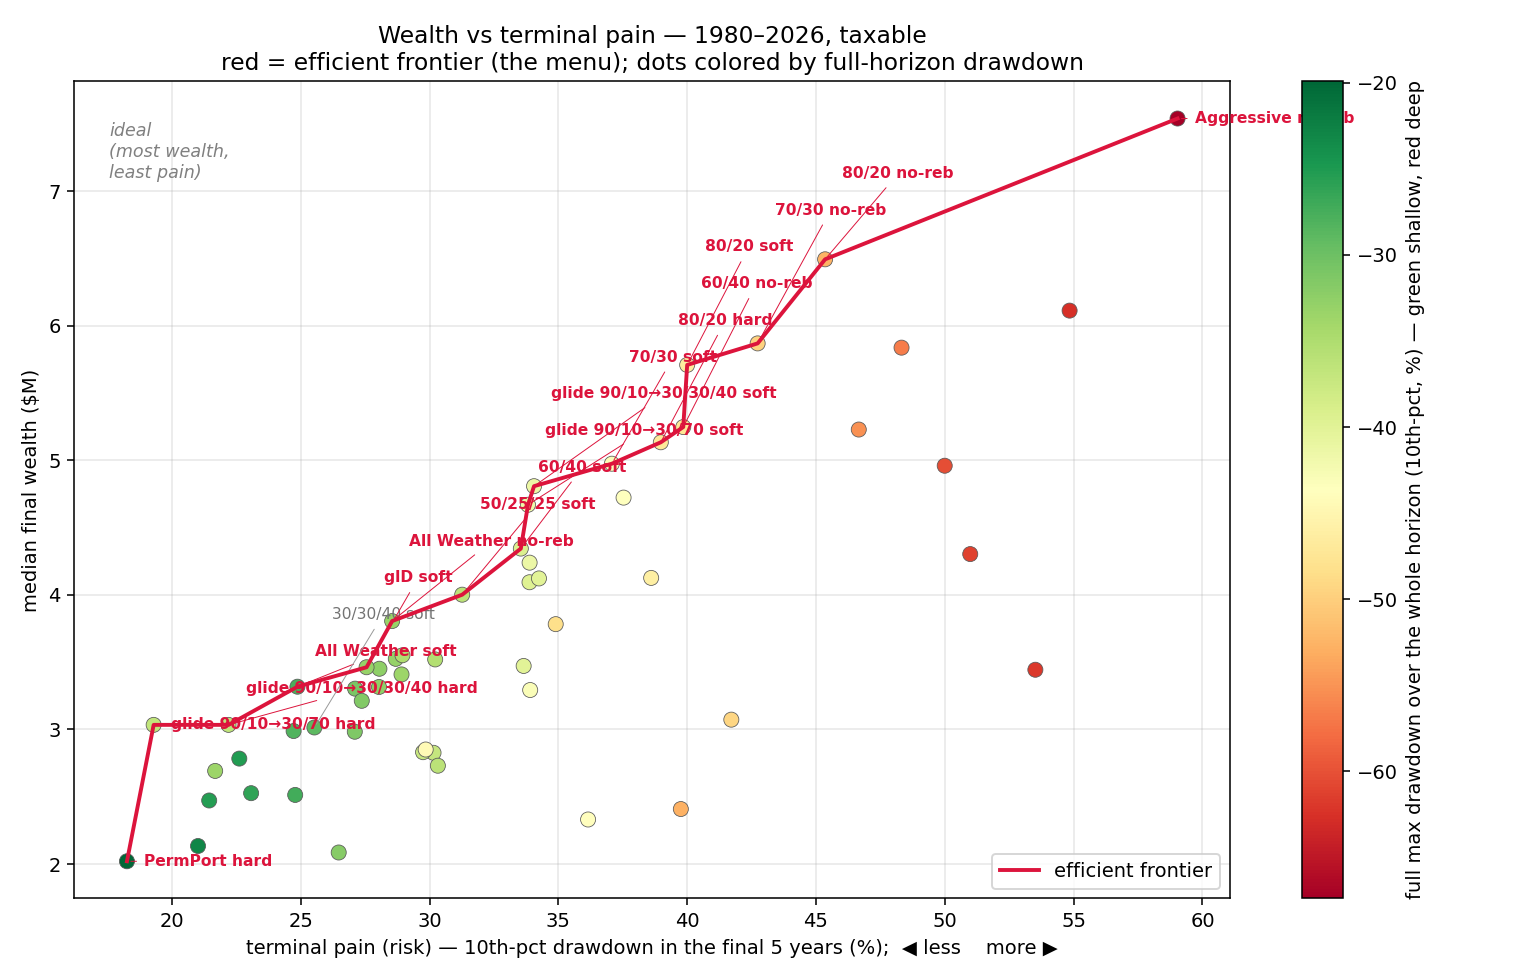
\includegraphics[width=0.92\textwidth]{results/frontier_1980_taxable.png}
\caption{Wealth versus terminal pain, taxable account, 1980--2026. Each dot is one strategy; the red
line is the efficient frontier. The ideal corner is top-left (most wealth, least pain).}
\label{fig:frontier_taxable}
\end{figure}

\begin{figure}[htbp]
\centering
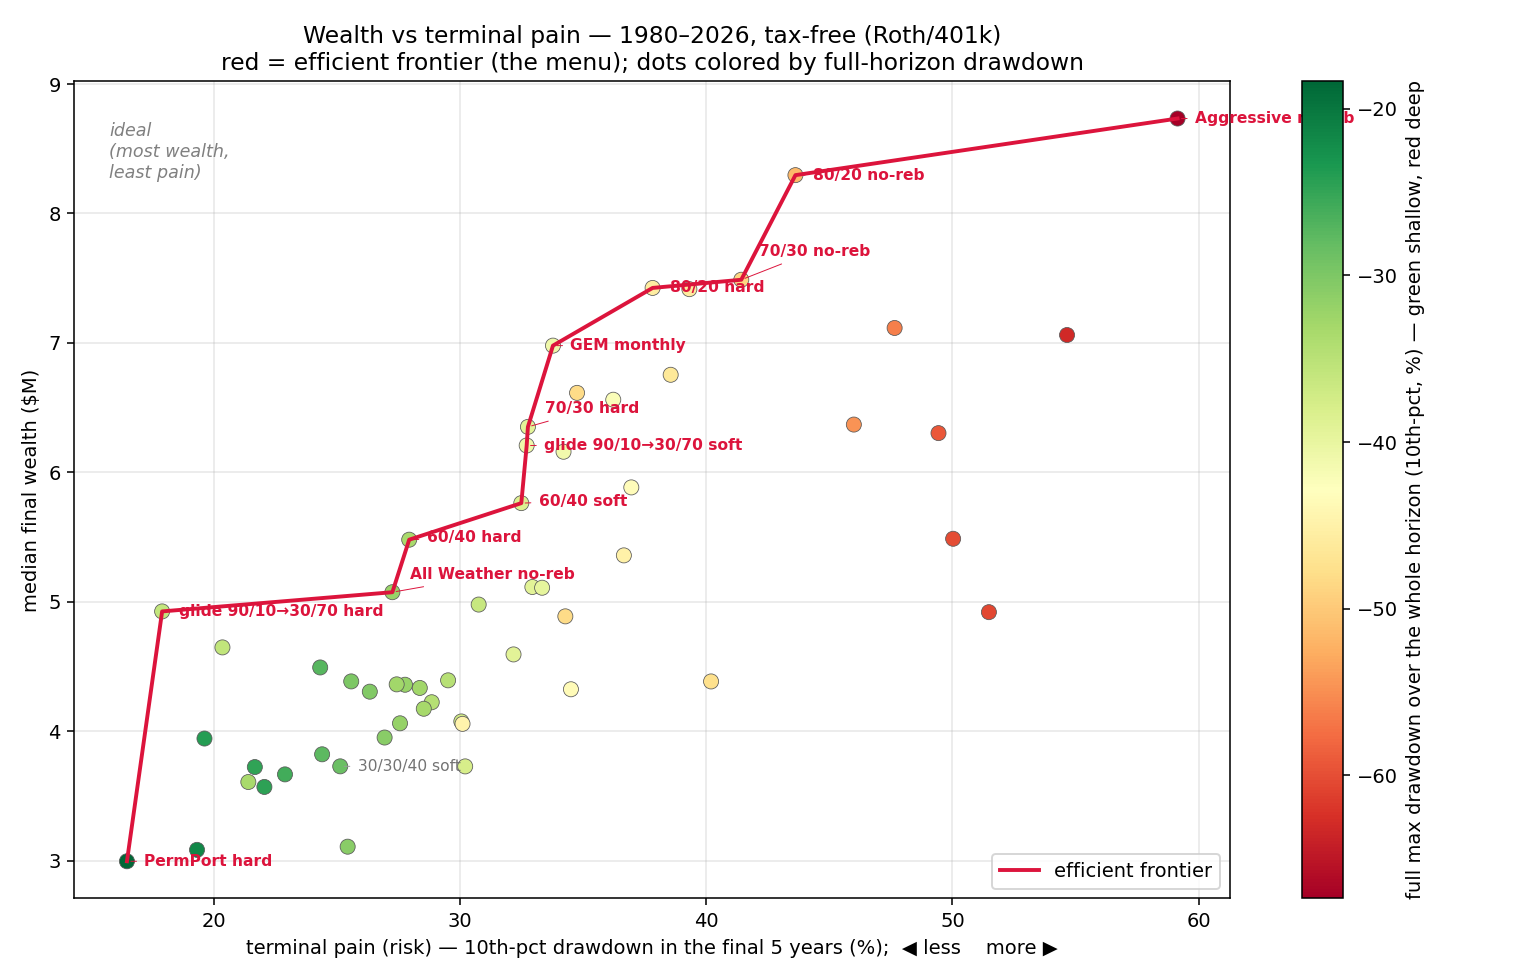
\includegraphics[width=0.92\textwidth]{results/frontier_1980_taxfree.png}
\caption{Wealth versus terminal pain, tax-free account, 1980--2026.}
\label{fig:frontier_taxfree}
\end{figure}

% ==========================================================================
% TODO (to build next, with language review):
%   - Questions a Careful Reader Will Ask (carry over + update for 1980-only, -30% cap)
%   - Calendar-year returns, income robustness appendices
% ==========================================================================

\section{What About Taking More Risk When Young?}\label{sec:youngrisk}

The most common objection to a steady allocation is that a young investor has decades ahead, so they
can take more risk early and dial it back as retirement nears. The first part is simply true: someone
in their twenties can absorb a deep loss, because there is time to recover. The question is the dialing
back. We test it directly: the standard target-date glide from about 90\% stocks down to a 30\% stock / 70\% bond
endpoint, run as a \emph{hard} rebalance (sells to hold the path) and a \emph{soft} version (redirects
new contributions only, never sells), plus a variant that ends at 30/30/40 (gold in the endpoint).

{\small
\begin{center}
\textit{Target-date glides vs.\ holding 30/30/40 flat, by account (median wealth and terminal pain,
1980--2026, 1{,}000 histories)}\\[2pt]
\begin{tabular}{@{}lrrrr@{}}
\toprule
 & \multicolumn{2}{c}{Tax-free} & \multicolumn{2}{c}{Taxable} \\
\cmidrule(lr){2-3}\cmidrule(lr){4-5}
Strategy & Wealth & Term.\ pain & Wealth & Term.\ pain \\
\midrule
Glide 90/10$\to$30/70, hard (stock/bond) & \$4.93M & $-18\%$ & \$3.22M & $-19\%$ \\
Glide 90/10$\to$30/70, soft (never sells) & \$6.21M & $-33\%$ & \$4.88M & $-34\%$ \\
Glide 90/10$\to$30/30/40, hard (gold endpoint) & \$4.65M & $-20\%$ & \$3.20M & $-22\%$ \\
Hold 30/30/40 throughout (soft) & \$3.73M & $-25\%$ & \$3.10M & $-25\%$\\
\bottomrule
\end{tabular}
\end{center}
}

\noindent The hard stock/bond glide is the most efficient strategy in the field -- the highest wealth
per unit of terminal pain in \emph{both} accounts (Section~\ref{sec:frontier}). It beats holding
30/30/40 flat on both axes in both accounts: in the taxable account \$\HardGlideTxWealth M against \$\FlatTxWealth M with a
shallower terminal pain ($-\HardGlideTxPain\%$ against $-\FlatTxPain\%$), and by more in the tax-free account (\$\HardGlideTfWealth M
against \$\FlatTfWealth M, $-\HardGlideTfPain\%$ against $-\FlatTfPain\%$). So ``risky
young, safe old,'' run as a rebalanced glide to a conservative endpoint, is supported here -- and unlike
some framings of the question, it holds up in the taxable account too, where the rebalancing is taxed,
not only in the shelter.

Three qualifications. First, it must be the \emph{hard} (rebalanced) glide. The soft version never
trims the early equity, so a large stock position compounds into retirement and the glide ends at
$-\SoftTDFPainLo\%$ to $-\SoftTDFPainHi\%$ terminal pain -- past the $-30\%$ threshold, and deeper than holding flat -- which
defeats a glide's purpose. Second, the efficient endpoint here is the plain 30/70 \emph{stock/bond}
mix: the variant that ends at 30/30/40, putting gold in the endpoint, is dominated by it -- the
de-risking, not the gold, is what lowers terminal pain in a glide. Third, the calm ending is bought
with a rougher youth: holding 90\% stocks early, the hard glide's 10th-percentile worst-case full
drawdown reaches $-\HardGlideDD\%$, against $-\FlatDD\%$ for holding flat. But that loss lands when the balance is
smallest, so in dollars it costs little, and it is gone before the balance is large enough for a
drawdown to remove serious money.

And suppose the investor carries the risk anyway. They often end with more money than the cautious one,
sometimes much more, even when a deep loss is never fully recovered. But that comparison is deceptive. A
large net worth at the peak is not an abstract number. It sets the house, the spending, the retirement
date, the commitments a person builds around what they believe they are worth. When a 50\% or 60\%
drawdown arrives, those commitments are hard to unwind, whatever the investor's appetite for risk.
Planning a retirement around \$5 million and arriving with \$3 million is still a comfortable retirement.
It is simply not the one that was planned for.

\section{Bonds from 1980--2026, and an Argument for Diversification}\label{sec:bonds}

Appendix~\ref{sec:calendar} shows that \emph{intermediate} bonds --- the dominant holding in the
target-date glide that tops the efficient frontier --- never suffered a severe drawdown across 1980--2026. Their
worst peak-to-trough fall was $-19\%$ (the 2022 rate spike), against $-55\%$ for US stocks, $-73\%$ for
REITs, and $-46\%$ for long Treasuries. For the intermediate-bond series the window is a four-decade bull
market, as rates fell from double digits toward zero, with 2022 the only setback.

The Monte Carlo resamples the 1980--2026 record. In that record intermediate bonds never had a severe
drawdown --- their worst was $-19\%$ (the 2022 rate spike), against $-55\%$ for stocks
(Appendix~\ref{sec:calendar}). The strategies that top the efficient frontier hold a high proportion of
bonds: \textbf{TDF 90/10$\to$30/70} ends at 70\% bonds at the point of largest balance, is efficient at
every horizon (Appendix~\ref{sec:horizon}), and carries terminal pain of $-\TdfHardPainLo\%$ to $-\TdfHardPainHi\%$. It holds
mostly the one asset that did not fall hard in this record.

The bond returns over this window reflect a decades-long fall in interest rates, from double digits
toward zero. The one bond decline in the record --- 2022, when long Treasuries fell $-46\%$ --- shows
what a sustained rising-rate or inflationary period could do to a bond-heavy portfolio, and no such
period is in the 1980--2026 record the Monte Carlo draws from.

The choice turns on what an investor believes about the future of bonds:
\begin{itemize}
\item If 46 years of bond history is a deep enough guide --- if the coming decades hold no bond drawdown
worse than anything in the record --- then \textbf{TDF 90/10$\to$30/70} is among the most efficient ways
to build wealth here, and the data support it.
\item If the investor will not hold 70\% bonds at the point of largest balance, near the end of the
horizon, they would instead take a \emph{diversified} mix that builds wealth within the $-30\%$ cap,
putting the defensive weight in gold \emph{and} bonds rather than bonds alone.
\end{itemize}

\noindent The rebalanced stocks/gold/bonds mixes are where that second investor would look. The
30/30/40, 40/30/30, and 40/25/35 mixes stay within the $-30\%$ cap at every horizon, in both accounts,
when rebalanced (Appendix~\ref{sec:horizon}). They build less wealth than the bond-heavy glide, but the
asset that has to hold up in a crisis is split between gold and bonds --- which need not fall together
--- rather than concentrated in bonds. Appendix~\ref{sec:horizon} lays out which mix, and soft versus
hard rebalancing, as a wealth-versus-pain trade.

\section{Why Stocks Only is Dangerously Wrong}\label{sec:concentration}

\begin{tcolorbox}[breakable, colback=blue!4!white, colframe=blue!50!black,
  title=\textbf{A scenario: one year from retirement, March 2020}]
You are a year from retirement. For a working lifetime you did what the most trusted advice in personal
finance says: you held the total US stock market, nothing else, and never sold. It worked --- your
balance is about \$\StockOnlyWealth M.

Then COVID arrives. In five weeks US stocks fall \CovidDD\%, and your account is worth \$\StockOnlyCovid M.
Every instinct you were taught says \emph{ride it out --- the market always comes back}. A quieter voice
says \emph{now, finally, move some to safety}. Ride it out, and you are betting you still have the years
for the recovery to arrive --- a year from retirement, you may not. Move to bonds now, and you sell a
third of your life's savings at the bottom, locking in the loss and missing the rebound. (COVID, as it
happened, recovered within months --- but at the bottom no one knew that, and the same fall had begun
the declines of 2000 and 2008.) There is no good answer. The decision that would have spared you was not
made in the crash; it was made, or missed, years earlier --- in how much you held in stocks as the
finish line came into view.

And \$\StockOnlyCovid M is still a fortune --- it just does not feel like one. The mind anchors on the
\$\StockOnlyWealth M of three weeks ago; what is felt is the third that vanished, at the one age with no
years left to rebuild. And the peak was never just a number --- it had set the retirement date, the
house, the spending, what would go to the children. \$\StockOnlyCovid M is a comfortable retirement; it
is simply not the one that was planned, arriving when nothing can be done about it.
\end{tcolorbox}

\begin{tcolorbox}[breakable, colback=blue!4!white, colframe=blue!50!black,
  title=\textbf{Eighteen months later: you held on, and you were right}]
You rode out March 2020, the market roared back, and through 2021 you sit at a fresh all-time high, a
year from retirement. Rattled by that March, you finally do what Collins prescribes for the home stretch
and move to his 75/25 --- the total stock market (VTSAX) and the total bond market (VBTLX). But there is
a catch the advice skips. After forty years of holding, about \GainFrac\% of your stock is embedded gain,
so the moment you sell, the tax is large --- and to reach a \emph{true} 75/25 you cannot sell just 25\%:
the tax comes out of the proceeds, leaving you nearer 80/20. So you sell about \FlipSalePct\% of the
stock and hand over roughly \$\FlipTax M, some \FlipTaxPct\% of your \$\StockOnlyWealth M, in
capital-gains tax. Voluntarily, at the peak, to feel safe.

Then 2022 --- your retirement year --- arrives, the one year in the record when stocks \emph{and} bonds
fell together. From the December high your 75/25 falls \SevenFiveDD\% to its low; add the tax you have
already paid and you are down \FlipTotalDD\% from where you started --- \emph{deeper} than the
\StockDD\% you would have suffered doing nothing at all. The move meant to protect you made the hole
bigger, because VBTLX, the very fund Collins names for safety, fell \BondDD\% right alongside stocks: the
cushion had nothing to cushion. (A diversified 30/30/40 fell \DivDD\% over the same months --- chiefly
because it held 30\% in stocks rather than 75\%, the rest spread across gold and bonds that did not all
bottom together.)

None of this means the instinct was wrong. At the cusp of retirement it is entirely reasonable to want
less pain. The lesson is narrower and sharper: a large, one-time conversion of a concentrated, low-basis
position is itself a risky act --- it crystallises a tax bill at whatever price the market happens to be,
and buys a cushion that may not cushion. The deeper point is that the safety a near-retiree wants is not
something bought at the end at all. It comes from holding a diversified mix --- a spread of assets that do
not move together --- \emph{at all times} through the accumulation, by whatever method suits the investor:
a static blend, soft rebalancing, hard rebalancing, or a glide. Diversify throughout, and there is never
a concentrated position to unwind, no forced sale at a peak, and the portfolio is already cushioned when the
bad year comes.
\end{tcolorbox}

That gap --- between the life planned at the peak and the life the market leaves --- is the risk this
report is built to limit, and it is the subject of this section. The advice that leads an investor to an
all-stock portfolio is not foolish; it is the mainstream, argued by its most credible advocates, and it
begins one step narrower still: with the idea that one could simply own the handful of great companies
that lead the market. The record of individual stocks is a caution against even that.

Cisco was not a speculative start-up. In March 2000 it was briefly the most valuable company in the
world --- profitable, and dominant in the internet's core networking equipment --- exactly the kind of
``quality'' name an investor would feel safe holding forever. Its shares still fell \CiscoDecline\% over
the following two and a half years, and did not regain their March 2000 price for more than
\CiscoRecoverYears\ years.

{\small
\begin{center}
\begin{tabular}{@{}lcccr@{}}
\toprule
Company & Peak & Trough & Decline & Time to recover \\
\midrule
Cisco & Mar 2000 & Oct 2002 & $-89\%$ & 25.7 yr \\
Meta & Sep 2021 & Nov 2022 & $-77\%$ & 2.4 yr \\
Netflix & Nov 2021 & May 2022 & $-76\%$ & 2.8 yr \\
Nvidia & Nov 2021 & Oct 2022 & $-66\%$ & 1.5 yr \\
Amazon & Jul 2021 & Dec 2022 & $-56\%$ & 2.8 yr \\
Alphabet & Nov 2021 & Nov 2022 & $-44\%$ & 2.2 yr \\
Microsoft & Nov 2021 & Nov 2022 & $-38\%$ & 1.6 yr \\
Apple & Dec 2024 & Apr 2025 & $-33\%$ & 0.8 yr\\
\bottomrule
\end{tabular}
\end{center}
}
\noindent\footnotesize Deepest drawdown by split-adjusted share price; time to recover is from the peak
back to that price. Cisco recovered earlier, in \CiscoTRRecoverYear, on a total-return basis with
dividends reinvested. Below Cisco, each row is that company's deepest fall within the last seven
years.\normalsize

\medskip
Nothing about being large, profitable, or dominant prevented Cisco's fall, and nothing exempts today's
leaders from the same possibility. Each of the seven largest technology companies has already fallen
between \BigTechMinDecline\% and \BigTechMaxDecline\% within the last seven years alone; that those
declines reversed within a few years, rather than a few decades, is a fact about the recent past, not a
guarantee.

The usual answer to this is not to pick stocks but to buy the whole market, and its most credible
advocates are emphatic about it. Warren Buffett's instruction for the trust he leaves his wife is to
``put 10\% of the cash in short-term government bonds and 90\% in a very low-cost S\&P 500 index
fund'';\footnote{Warren E.\ Buffett, Berkshire Hathaway Inc.\ 2013 Letter to Shareholders.} John Bogle,
who built the first index fund, reduced it to ``don't look for the needle in the haystack --- just buy
the haystack.''\footnote{John C.\ Bogle, \emph{The Little Book of Common Sense Investing} (Wiley, 2007).}
On the record above we agree: owning the broad index has beaten owning the names inside it. The question
is what the haystack now holds.

The exposure is also far greater than it was at the last technology peak. The Nasdaq-100 --- essentially
the large technology names --- is now about \$\NdxMktcap\ trillion, roughly \NdxShareNow\% of the
\$\UsMktcap\ trillion total US market; the ten largest stocks alone are about \TopTenNow\% of the S\&P
500, against roughly \TopTenThen\% at the 2000 peak.\footnote{These market-concentration figures are as
of \ConcAsOf{} and, unlike the drawdowns in this section, are not computed from price data: \ConcSources}
A repeat of the dot-com decline --- the Nasdaq-100,
which an investor could buy as the QQQ fund from March 1999, fell about \NasdaqDotcomDecline\% into 2002
and took roughly \NasdaqDotcomRecoverYears\ years to regain its price --- would, from a \NdxShareNow\%
weight, erase on the order of \EraseNow\% of the
entire US market even if every other stock held flat, and more once they did not. In 2000 that same
index was only about a third of the market, so an identical decline subtracted closer to \EraseThen\%
and the rest of the market cushioned the blow; today there is far less to cushion with --- the
concentrated bet has become the index itself. This is the risk the diversification of
Section~\ref{sec:assetselection} is meant to blunt, and the reason the diversified portfolio holds only
30\% in stocks: a shock of that kind strikes a fraction of the portfolio rather than the bulk of it.

The most emphatic popular case for stocks is JL Collins's. In \emph{The Simple Path to Wealth} and his
widely read ``Stock Series,'' he tells the investor building wealth to own one thing --- the total US
stock market, through the fund VTSAX --- and to hold it through every crash without selling. His image
is Odysseus and the Sirens: ``tie yourself to the mast and stay the course,'' he writes, because ``the
market always recovers and resumes its relentless rise''; if you cannot do that, he says plainly, this
way of investing is not for you.\footnote{JL Collins, \emph{The Simple Path to Wealth} (2016); the
``Stock Series'' at jlcollinsnh.com.} To be fair, he is not against bonds --- once the investor stops
working and lives on the portfolio, he shifts to roughly 75\% stocks and 25\% bonds to smooth the
ride.\footnote{JL Collins, ``Stocks --- Part XXIII: Selecting Your Asset Allocation,'' jlcollinsnh.com
(2014).} But through the accumulation years --- the whole span this study covers --- he is unambiguous:
hold stocks, very nearly only stocks, and sit through the drops.

The mast holds because the storm passes, and that logic is sound --- while there is time for the storm
to pass. The objection here is not the one Collins answers. It is not whether the investor can
\emph{tolerate} a deep drop; an investor with perfect nerve still should not carry an all-stock portfolio
into the last years of accumulation. The reason is timing, not temperament. Terminal pain --- this
report's main risk measure --- is the 10th-percentile drawdown over the final five years before
retirement, when the balance is at its largest and the years left to recover are gone. Run through the
same 1980--2026 Monte Carlo as every other figure here, a 100\%-US-stock portfolio carries terminal pain of
about $-\StockOnlyPain\%$, against $-\DivPain\%$ for the diversified 30/30/40 --- nearly twice as deep
--- in exchange for a higher median wealth
(\$\StockOnlyWealth M versus \$\DivWealth M). Early in accumulation a fall like that is survivable: the
balance is small, the monthly contributions keep buying, and the storm passes with decades to spare.
Close to the end it may pass too late. The recovery can arrive after the money was needed --- after the
paychecks stop and the withdrawals begin --- and a paper loss that would have healed in time becomes a
permanent cut to the retirement it was meant to fund.

And sometimes the storm does not pass on any human schedule. ``The market always recovers'' describes US
history; it is not a law that holds everywhere. Japan's Nikkei~225 peaked at the end of \JapanPeakYear,
fell \JapanDecline\% to its \JapanTroughYear\ low, and did not close back above its \JapanPeakYear\ high
until \JapanRecoverYear{} --- \JapanRecoverYears\ years later.\footnote{\JapanSource} An investor who
tied himself to that mast at the peak waited more than three decades just to break even on price.

This is why the argument of this report is for diversification \emph{across} assets that do not move
together, not only \emph{within} one of them. Collins's own shift to bonds in retirement grants the
principle; the difference is that the diversified mixes here hold that spread from the start, and split
the defensive weight between gold and bonds rather than bonds alone. Ray Dalio calls a portfolio of fifteen or twenty uncorrelated return streams
the ``Holy Grail of investing,'' because combining them can cut risk sharply without giving up expected
return.\footnote{Ray Dalio, \emph{Principles} (Simon \& Schuster, 2017). Dalio's own All Weather
portfolio is itself bond-heavy --- in this study 40\% long Treasuries and 15\% intermediate bonds,
against 30\% stocks and 15\% gold --- and it is among the efficient strategies in the backtest
(Section~\ref{sec:frontier}). That showing, though, owes much to the 1980--2026 bond bull
(Section~\ref{sec:bonds}); the same long-Treasury weight that carried it is what would expose it to the
rising-rate shock that struck in 2022.} A broad stock index
diversifies away the risk that any one company fails; it does nothing about the risk that stocks as a
class have a decade --- or, as in Japan, a generation --- that does not come back. That is the gap the
gold and bond holdings are there to cover.

\paragraph{What if you sell out of stocks just before retirement?} Stocks build the most
wealth, but at the cost of terminal pain. So we tested a middle-ground strategy ---
a staged \emph{wind-down to cash}. The investor stays fully in US stock until five years before
retirement, then sells it off in yearly steps: half to begin with, and the rest run down evenly over
the years that follow --- a fifth of what remains, then a quarter, a third, a half, and finally all of
it --- so the portfolio is entirely in cash by retirement, while the monthly contributions keep buying
stock the whole way. The idea echoes Wade Pfau's
rising-equity-glidepath work,
which holds a defensive ``bond tent'' of cash and bonds through the fragile years around retirement
and then ramps equity back up afterward.\footnote{Wade Pfau and Michael Kitces, ``Reducing Retirement
Risk with a Rising Equity Glide Path,'' \emph{Journal of Financial Planning} (2014).} We model only
the run-up to retirement, not the post-retirement portfolio. We also test two variations: selling 60\%
to begin with, with later contributions still buying stock; and selling 40\% to begin with, with later
contributions going to cash instead. All three are in Appendix~\ref{sec:winddown}.

On the same 1980--2026 simulation as the rest of the report, all three wind-downs trade wealth for
lower terminal pain, in both accounts (Table~\ref{tab:winddown}). The portfolio ends in cash, which does
not fall, so terminal pain drops; and the all-stock portfolio carried into the wind-down is, after four
decades of compounding, almost all gain, so selling it down realizes that gain. The gap between the two
accounts is the capital-gains tax --- waived in a tax-sheltered account, owed in full in a taxable one.

\begin{table}[h]
\centering
\caption{Wind-down terminal pain and median final wealth, by version and account, 1980--2026.}
\label{tab:winddown}
{\small\begin{tabular}{@{}lcccc@{}}
\toprule
 & \multicolumn{2}{c}{Taxable} & \multicolumn{2}{c}{Tax-free} \\
\cmidrule(lr){2-3} \cmidrule(lr){4-5}
Strategy & Terminal pain & Median wealth & Terminal pain & Median wealth \\
\midrule
100\% US stock & $-49\%$ & \$8.01 M & $-48\%$ & \$9.79 M \\
Wind-down, sell 50\% & $-31\%$ & \$5.13 M & $-25\%$ & \$7.77 M \\
Wind-down, sell 60\% & $-32\%$ & \$4.96 M & $-24\%$ & \$7.51 M \\
Wind-down, sell 40\% & $-32\%$ & \$5.24 M & $-27\%$ & \$7.90 M\\
\bottomrule
\end{tabular}}
\end{table}

The same wealth-against-terminal-pain test used throughout, with the $-30\%$ cap of
Section~\ref{sec:frontier}, separates the two accounts. In a tax-free account all three wind-downs are
\emph{efficient} --- not beaten by any of the 56 strategies on both wealth and terminal pain at once ---
and stay within it, so all three sit on the efficient frontier in the tax-free account. In
a taxable account none do: each one's terminal pain ($-31\%$ to $-32\%$) is past the cap, so the
strategy is ruled out before efficiency even comes into play. The full figures for both accounts are in
Appendix~\ref{sec:winddown}.

\section{Questions a Careful Reader Will Ask}\label{sec:critiques}

\paragraph{Aren't these just the funds that happened to perform best, chosen with hindsight?}
Some hindsight is unavoidable: we choose the portfolio in 2026 knowing how the decades turned out, as
the asset-selection section concedes. The defense is that the portfolios are deliberately un-clever ---
each holds roughly equal amounts across a few broad asset classes rather than a concentrated bet on the
known winner --- and the central finding, that drawdown depth tracks equity weight, is structural rather
than a forecast. The numbers are directional; reproduce them before relying on a specific figure.

\paragraph{Are these nominal or real (inflation-adjusted) dollars?}
Nominal --- and that is the right unit. The investor reads their account balance in
nominal dollars, and the household-wealth figures we compare against are reported in nominal dollars of the same
vintage, so the comparison is like-for-like with no adjustment needed. More to the point, nothing in the
conclusions turns on the distinction: drawdowns are percentages, the risk-adjusted measures are ratios,
and the ranking of the mixes and the drawdown ceiling are relative quantities --- all of which a common
inflation deflator leaves unchanged. Restating the whole study in real terms would shrink every balance
by the same factor and reorder nothing: the safest mix is still safest, and the gaps are still the gaps.
Inflation matters greatly for a different question --- whether a given sum is \emph{enough to live on}
decades hence --- but that is one of purchasing power, separate from which mix the money should go into.

\paragraph{It is still one historical period --- doesn't the Monte Carlo just reshuffle 1980--2026?} The
window is 46 years, and far from a quiet one: it spans the double-digit inflation of the early 1980s and
its collapse, the 1987 crash, the dot-com boom and bust, the 2008 financial crisis, the 2020 pandemic,
and the 2022 rate shock --- most of the regimes a modern investor would worry about. The block bootstrap
draws contiguous runs of random length --- from a month to about two and a half years --- keeping the
real structure of crashes, recoveries, and sustained trends intact while varying \emph{when} they
strike. Drawing a thousand such reorderings and scoring each
strategy on the resulting \emph{distribution} --- its median final wealth, and its terminal pain, the
10th percentile of the final-five-year drawdown --- measures the strategy across many plausible sequences
rather than the single one that happened to occur. The efficient frontier is built on that distribution,
so the ranking is a property of the spread of outcomes, not of the lucky order in which 1980--2026 fell.
The one thing no resampling can do is produce a future with no analog in the record, a regime the last
half-century never saw; that is the limit of any method built on history, not a quirk of this study. Section~\ref{sec:bonds} takes up the case where it
matters most for the rankings: intermediate bonds never fell hard in this window, so the simulation
cannot show them falling hard, and the bond-heavy strategies look safer than a serious bond decline could
prove them to be.

\paragraph{Would a shorter accumulation horizon change which strategies win?} We recomputed the efficient
set at five shorter horizons --- 31, 35, 38, 40, and 44 years (Appendix~\ref{sec:horizon}). Two strategies stayed on
the efficient frontier at every one, in both accounts: the 90/10$\to$30/70 target-date glide (hard) and
the Permanent Portfolio (hard). A wider group never left the \emph{viable} region --- terminal pain
within the $-30\%$ cap --- at any horizon: the rebalanced diversified mixes that hold equity to about
40\% or less (30/30/40, 40/30/30, 40/25/35, the Permanent Portfolio, All Weather) and the glides that
rebalance down to a conservative endpoint. A shorter horizon leaves equity less time to recover from a
deep crash, so the more equity a strategy carries, the more a late crash costs. The shorter the horizon, then, the stronger the case for carrying less equity --- or for
actively gliding down to it as retirement nears.

\paragraph{Several series use proxy or constructed data before the mid-1990s.} They do. International
stocks and technology use proxy funds of the same class; long Treasuries and cash before their funds
(1986 and 1991) are constructed from constant-maturity Treasury yields; and REITs before 1986 use the
monthly Nareit index distributed across trading days. The REIT pre-1986 daily path is therefore
interpolated and does not carry day-to-day volatility -- the one series whose pre-fund daily path is
synthetic at the daily frequency. The construction is set out in Appendix~\ref{sec:datamethod}; strategies
that depend on these earlier-than-fund series carry the corresponding caveat.

\paragraph{Isn't the $-30\%$ terminal-pain threshold arbitrary?} It is a value judgment, but a reasoned
one, not an arbitrary cutoff. Section~\ref{sec:frontier} gives the basis: a drawdown beyond roughly
$30\%$ suffered near retirement --- with little time and no fresh income to rebuild from --- is one we
judge likely to be unrecoverable for an investor who has built a lifestyle around their expected wealth,
so we weight avoiding it above the extra wealth a riskier mix can earn. Another investor could
reasonably place the line at $-25\%$ or $-35\%$; the point is that it follows from a stated principle,
and we make ours explicit. The threshold also does not change the efficient frontier itself -- the set
of strategies not beaten by another on both wealth and drawdown -- only which of them an investor would
consider tolerable; we report the full distribution so a reader can apply a different ceiling.
Strategies whose terminal pain sits within a few points of $-30\%$ move on and off the within-threshold
set as the random seed changes, so we treat those as borderline and rest the conclusions on the
strategies comfortably inside.

\paragraph{Ranking by wealth over terminal pain is just one choice of metric.} Correct, and we use it
only to \emph{order} strategies that are already on the frontier. The frontier itself is metric-free:
no strategy on it is beaten on both axes at once. Different objectives select different members of the
same set -- the most wealth, the calmest, the best risk-adjusted -- which is why all of them are
reported rather than a single winner.

\paragraph{Why fixed weights rather than an optimization?} A mean-variance optimization would require
forecasting returns and correlations we do not claim to know, and would itself be fit to this one
period. Fixed broad weights apply the diversification principle without that forecast. The cost is that
the weights are not tuned; the benefit is that they are not over-fit.

\paragraph{Don't some of the winners depend on the specific period?} Yes, and we flag the two clearest
cases. All Weather's risk-adjusted standing leans on long-Treasury returns over a window in which rates
fell a long way; and the target-date glide minimizes drawdown in the final five years, which is the very
quantity the terminal-pain metric measures, so a glide scoring well on it is partly built in. The robust
conclusions are the patterns that survive the second seed, not any single strategy's rank.

\paragraph{The taxes are stylized.} Flat rates and two idealized account types, fully taxable and fully
tax-free (Appendix~\ref{sec:datamethod}). Real taxation has brackets, state differences, and separate
schedules for qualified dividends and long-term gains. The after-tax figures are therefore directional
-- the ordering of strategies and the rough magnitude of the tax drag -- not a precise dollar outcome
for any individual.

\appendix

\section{Data and Method}\label{sec:datamethod}

\paragraph{Price series.} Each asset is the total-return series of a low-cost fund --- adjusted closing
prices with dividends reinvested --- extended before that fund's inception by a proxy fund or a
constructed series of the same type. A proxy is joined at the fund's first trading date by scaling it
to match the fund's level there, so returns are continuous and the real fund takes over as soon as it
exists. A proxy-to-fund switch is treated as a tax-free in-kind exchange: the strategy continues to
hold that one asset, so no sale occurs and no capital gain is realized; only the underlying dividends
and interest, from whichever fund is live, are taxed. Gold is the LBMA afternoon (PM) fix, a spot
price with no income; held through a physical-bullion ETF, it carries the management fee under Costs.

{\small
\begin{center}
\begin{tabular}{@{}lll@{}}
\toprule
Asset class & Fund (from inception) & Earlier series \\
\midrule
US large-cap stocks & VFINX (1980), then SPY & --- \\
US technology & RYOCX Nasdaq-100 (1994), then QQQ (1999) & broad US stocks before 1994 \\
International stocks & VGTSX (Apr 1996) & SCINX / PRITX / VTRIX proxies \\
Real estate (REITs) & FRESX (1986), then VGSIX (1996) & FTSE Nareit All-Equity index, 1980--86 \\
US aggregate bonds & VBMFX (Dec 1986) & FGOVX, 1980--86 \\
Long Treasuries & VUSTX (May 1986) & 30-yr constant-maturity yield, 1980--86 \\
Short Treasuries (cash) & VFISX (Oct 1991) & 13-wk T-bill rate, 1980--91 \\
Gold & LBMA PM fix (spot) & --- \\
\bottomrule
\end{tabular}
\end{center}
}

\paragraph{Constructed Treasury and REIT series.} Three series have no investable fund reaching back to
1980, so their pre-fund segment is constructed from a published index and then spliced (tax-free, as
above) into the real fund.
\begin{itemize}
\item \textbf{Long Treasuries} (to May 1986) and \textbf{cash / short Treasuries} (to Oct 1991) are
built from the published constant-maturity Treasury yield --- the 30-year for long, the 13-week
T-bill for cash. Each day we hold a par Treasury at that maturity and reprice it at the next day's
yield; the coupon accrual is the taxable income and the price change is capital. The matching fund's
expense ratio (0.2\%/yr) is applied as a daily drag over the constructed segment, the same way the
gold fee is applied. After the splice the real fund's net-of-fee returns apply.
\item \textbf{REITs} (to Nov 1986) use the FTSE Nareit All-Equity monthly total-return
index;\footnote{FTSE Nareit U.S. Real Estate Index Series, monthly historical returns, Nareit
(reit.com).} each month's total return is distributed across that month's trading days, with the
income component split out as taxable, net of a REIT-fund expense ratio (0.7\%/yr), then spliced into
the FRESX$\to$VGSIX fund chain. \emph{Limitation:} no daily REIT series exists before 1986, so the
1980--86 daily path is interpolated from monthly data and does not carry day-to-day volatility. This
is the one series whose pre-fund daily path is synthetic at the daily frequency.
\end{itemize}
Pre-1996 international and technology use proxy \emph{funds} of the same class (no construction). The
strategies that depend on these earlier-than-fund series carry the corresponding caveat.

\paragraph{Income and dividends.} Interest and dividends come from each fund's actual per-share
distribution records, captured at their real dates and amounts; for the constructed Treasury and REIT
segments, the income component of the construction above. These drive the income tax below.

\paragraph{Costs.} The gold holding carries a \textbf{0.4\% annual management fee} (a physical-bullion ETF
expense ratio), accrued daily as a drag on its value; it is an expense, not a sale, so it realizes no
capital gain. The constructed long-Treasury, cash, and REIT segments carry the expense ratio of the
fund they splice into (0.2\% for the Treasuries, 0.7\% for REITs), applied the same way over the
pre-fund segment. Every purchase and every sale pays a \textbf{0.1\% transaction cost} --- each monthly
contribution, each hard rebalance, each momentum switch, and each sale made to raise a tax payment. The
no-rebalance and soft mixes trade only incoming contributions and bear this lightly; the hard-rebalanced
and momentum strategies turn over more and bear it most. All cost rates are configurable parameters.

\paragraph{Contributions and window.} The investor contributes 20\% of gross salary on the first
trading day on or after the 15th of each month, with salary set by the $75^{\text{th}}$-percentile
anchors of \S\ref{sec:about}. All strategies run on \textbf{1980--2026}.

\paragraph{Monte Carlo.} Alternative histories are built by a block bootstrap: contiguous blocks of
random length (22 to 600 trading days) are drawn with replacement from the real history and stitched
together until the window is filled. Each day's price return and its dividend yield are resampled
\emph{together}, so the income structure travels with the price structure. We draw 1{,}000 paths from a
fixed seed, and re-ran the full Monte Carlo under a second independent seed; the efficient set
(Section~\ref{sec:frontier}) is unchanged in both accounts, with only strategies sitting at the $-30\%$
threshold moving across it.

\paragraph{Dividends in the resampled paths.} Real dividends are discrete events --- monthly for bonds
and Treasuries, quarterly for stocks and the REIT, semiannual for international, none for gold.
Shuffling days makes the \emph{number} of ex-dates in a synthetic year random: a year can carry more
dividend events than the asset ever pays, or fewer. To keep the paths realistic, we changed the
dividend event days to match each asset's real payment cadence. For each asset-year we sum the dividend
the strategy actually collected ---
yield times shares held times price, day by day across the year --- and re-lay that received total as
the asset's usual number of evenly spaced, equal-dollar payments, backing out the per-day yield from
the share balance and price where each lands. Because receipt depends on the share balance, which the
contributions grow through the year, the re-bin is applied in-run as two passes: the first records the
share path, the second re-spaces against it. A year that received nothing stays empty: a sampled year
can genuinely collect no dividends --- QQQ paid none until 2003, gold none ever --- so we leave it at
zero rather than manufacture one. Because we did not change the
annual dividend amounts in these paths, our changes do not impact the actual returns or taxes in either
account.

\paragraph{Taxes --- and why they are directional.} The tax model below applies to a fully taxable
account. The report also runs every strategy in a fully tax-free account (Roth or 401k), where these
taxes are waived; the account-aware comparison covers the two. \emph{Income} is taxed each year: bond and Treasury interest at 20\% (Treasury interest is largely
state-exempt, which lowers its effective rate), stock dividends and REIT distributions at 25\%, gold
nothing. It is accrued per asset by calendar year and paid the following January by selling that same
asset. \emph{Realized capital gains} --- from the hard-reset rebalancing (a variant of every static mix
here) and the momentum strategy's switches --- are taxed at 25\% the same way; the soft-rebalanced and
buy-and-hold strategies never sell to rebalance, so their only tax is on income.

Real taxation is far more intricate than this. Brackets rise with income, states differ, long- and
short-term gains run on separate schedules, dividends split into qualified and non-qualified, the net
investment income tax applies above certain thresholds, and holding an asset in a taxable versus a
tax-deferred account changes everything. We deliberately use flat rates and two stylized account types
--- fully taxable and fully tax-free. The
after-tax figures should therefore be read as \textbf{directional}: they show the \emph{ordering} of
the strategies and the rough \emph{magnitude} of the tax drag --- which mixes are hit hardest --- not a
precise dollar outcome for any individual.

\section{Calendar-Year Returns and Diversification, 1980--2026}\label{sec:calendar}

\noindent Annual total returns for each asset (stocks and bonds include dividends; gold is price) and for
the 30/30/40 mix. The blend column is the soft 30/30/40's \textbf{time-weighted return (TWR)} each
year: from the strategy's actual value path, we remove each day's contribution before measuring the
daily return, then compound those over the year. (1980 is measured from January~15 and 2026 is
year-to-date through June~1.) The blend is a weighted combination of the assets, so its return in any
year is mechanically the sum of the assets' returns at their weights -- which is what lets the other
assets cushion a fall in one.

{\footnotesize
\begin{center}
\begin{minipage}[t]{0.46\textwidth}
\begin{tabular}{@{}rrrrr@{}}
\toprule
Year & Stocks & Gold & Bonds & 30/30/40 \\
\midrule
1980 & 24.4 & $-13.8$ & 6.8 & 7.9 \\
1981 & $-8.6$ & $-32.6$ & 10.8 & $-9.7$ \\
1982 & 19.3 & 14.9 & 26.5 & 20.9 \\
1983 & 17.1 & $-16.3$ & 3.2 & 0.0 \\
1984 & 3.7 & $-19.4$ & 11.4 & $-1.7$ \\
1985 & 22.6 & 6.0 & 17.9 & 14.4 \\
1986 & 9.3 & 19.0 & 14.1 & 13.1 \\
1987 & 4.7 & 24.5 & 1.6 & 9.0 \\
1988 & 16.3 & $-15.3$ & 7.4 & 1.4 \\
1989 & 31.4 & $-2.8$ & 13.7 & 12.8 \\
1990 & $-3.3$ & $-3.1$ & 8.7 & 0.4 \\
1991 & 30.2 & $-8.6$ & 15.3 & 11.4 \\
1992 & 8.2 & $-5.7$ & 7.3 & 2.7 \\
1993 & 9.1 & 17.7 & 9.7 & 10.9 \\
1994 & 1.2 & $-2.2$ & $-2.6$ & $-2.2$ \\
1995 & 37.4 & 1.0 & 18.3 & 17.5 \\
1996 & 22.9 & $-4.6$ & 3.6 & 6.6 \\
1997 & 33.2 & $-21.4$ & 9.5 & 9.1 \\
1998 & 28.6 & $-0.8$ & 8.6 & 14.0 \\
1999 & 21.1 & 0.9 & $-0.7$ & 8.4 \\
2000 & $-9.1$ & $-5.4$ & 11.4 & $-1.9$ \\
2001 & $-12.0$ & 0.7 & 8.4 & $-2.4$ \\
2002 & $-22.2$ & 25.6 & 8.4 & 0.1\\
\bottomrule
\end{tabular}
\end{minipage}\hfill
\begin{minipage}[t]{0.46\textwidth}
\begin{tabular}{@{}rrrrr@{}}
\toprule
Year & Stocks & Gold & Bonds & 30/30/40 \\
\midrule
2003 & 28.5 & 19.9 & 3.9 & 14.8 \\
2004 & 10.7 & 4.6 & 4.3 & 5.8 \\
2005 & 4.8 & 17.8 & 2.4 & 7.1 \\
2006 & 15.6 & 23.2 & 4.3 & 13.2 \\
2007 & 5.4 & 31.9 & 7.0 & 14.3 \\
2008 & $-37.0$ & 4.3 & 5.1 & $-7.5$ \\
2009 & 26.5 & 25.0 & 6.0 & 17.2 \\
2010 & 14.9 & 29.2 & 6.3 & 17.5 \\
2011 & 2.0 & 8.9 & 7.6 & 6.5 \\
2012 & 15.8 & 8.3 & 4.1 & 7.9 \\
2013 & 32.2 & $-27.3$ & $-2.2$ & $-6.7$ \\
2014 & 13.5 & 0.1 & 5.8 & 5.7 \\
2015 & 1.2 & $-12.1$ & 0.3 & $-3.9$ \\
2016 & 11.8 & 8.1 & 2.5 & 6.8 \\
2017 & 21.7 & 12.7 & 3.5 & 12.0 \\
2018 & $-4.5$ & $-0.9$ & $-0.1$ & $-2.4$ \\
2019 & 31.3 & 18.4 & 8.6 & 19.1 \\
2020 & 18.2 & 24.6 & 7.6 & 16.1 \\
2021 & 28.5 & $-4.3$ & $-1.7$ & 8.7 \\
2022 & $-18.2$ & 0.4 & $-13.2$ & $-12.0$ \\
2023 & 26.1 & 14.6 & 5.6 & 16.4 \\
2024 & 24.8 & 25.5 & 1.1 & 18.5 \\
2025 & 17.7 & 67.4 & 6.7 & 30.4 \\
2026 & 11.5 & 1.9 & 0.4 & 5.2\\
\bottomrule
\end{tabular}
\end{minipage}
\end{center}
}

\begin{figure}[htbp]
\centering
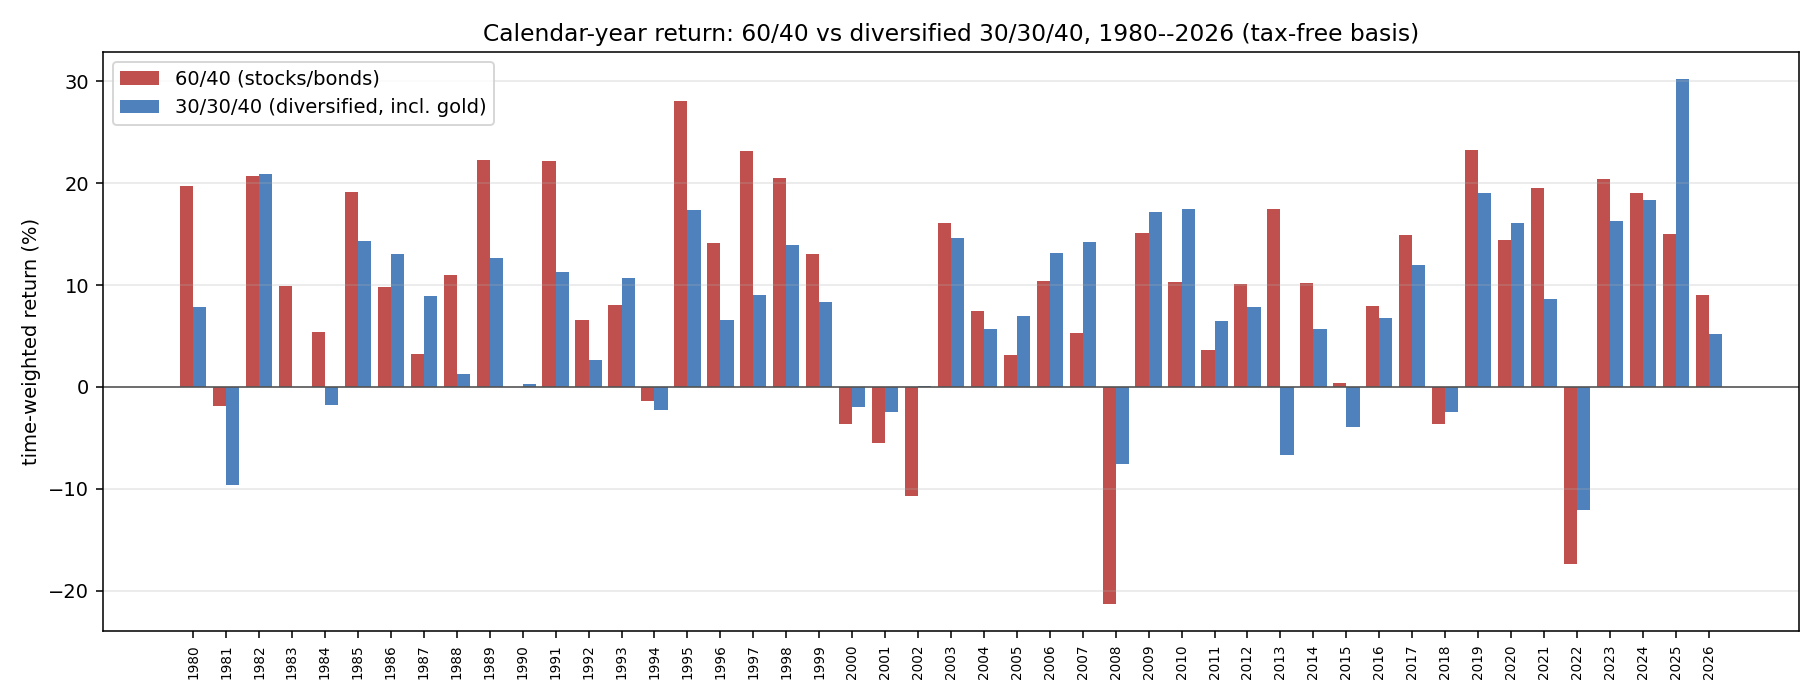
\includegraphics[width=0.95\textwidth]{results/calendar_60_40_vs_div.png}
\caption{Calendar-year return, 60/40 (stocks/bonds) versus diversified 30/30/40 (with gold), 1980--2026.
In the years the stock/bond mix fell hardest, the diversified mix fell less.}
\label{fig:calendar}
\end{figure}

\paragraph{The diversification benefit, in the years it mattered.} 60/40 had eight down years over the
window. The table below sets them beside gold's return that year and the diversified 30/30/40:

{\small
\begin{center}
\begin{tabular}{@{}rrrr@{}}
\toprule
Year & Gold & 60/40 & 30/30/40 \\
\midrule
1981 & $-32.6$ & $-1.9$ & $-9.7$ \\
1990 & $-3.1$ & $-0.0$ & $0.3$ \\
1994 & $-2.2$ & $-1.4$ & $-2.3$ \\
2000 & $-5.4$ & $-3.7$ & $-2.0$ \\
2001 & $0.7$ & $-5.5$ & $-2.5$ \\
2002 & $25.6$ & $-10.7$ & $0.1$ \\
2008 & $4.3$ & $-21.3$ & $-7.6$ \\
2018 & $-0.9$ & $-3.6$ & $-2.4$ \\
2022 & $0.4$ & $-17.4$ & $-12.1$\\
\bottomrule
\end{tabular}
\end{center}
}

In the three worst years for a stock/bond portfolio -- 2008 ($-21\%$), 2002 ($-11\%$), and 2022
($-17\%$) -- gold was flat or up, and the diversified 30/30/40 fell much less ($-7.5\%$, $+0.1\%$,
$-12.0\%$). 2022 is the pointed case: it is the one year in the window stocks \emph{and} bonds fell
together, the scenario a 60/40 has no defense against, and the gold holding is what cushioned the
diversified mix. The benefit is not automatic every year: in 1981 gold fell 33\% and the diversified
mix fell more than 60/40; and the diversifier matters -- All Weather's long Treasuries cushioned 2008
(it fell only $-1.8\%$) but deepened 2022 (it fell $-19.1\%$, worse than 60/40), because long-duration
bonds rallied in the 2008 flight to quality and crashed in the 2022 rate spike. The 30/30/40 mix shown
here is \emph{not} on the efficient frontier -- it is dominated on the long-run wealth-versus-pain trade
-- but it illustrates the point plainly: spreading risk across assets that do not all fall together
cushions the years that hurt the most. No one can predict the future; but a repeat of a 2022-type year
would, on this evidence, be expected to hurt a concentrated stock/bond mix more than a gold-holding
diversified one.

\paragraph{Worst drawdown by asset class.} The single deepest peak-to-trough fall each asset suffered
over the window (daily total return) is uneven, and the unevenness matters for what follows:

{\small
\begin{center}
\begin{tabular}{@{}lrcr@{}}
\toprule
Asset class & Worst drawdown & Period & Underwater \\
\midrule
US stocks & $-55\%$ & 2007--2009 & 5 yr \\
Intermediate bonds & $-19\%$ & 2020--2022 & 6 yr$^{*}$ \\
Long Treasuries & $-46\%$ & 2020--2023 & 6 yr$^{*}$ \\
Gold & $-70\%$ & 1980--1999 & 28 yr \\
REITs & $-73\%$ & 2007--2009 & 6 yr\\
\bottomrule
\end{tabular}
\end{center}
}
\noindent\footnotesize $^{*}$Still below the prior peak at the window's end (June 2026).\normalsize\
US stocks, REITs, gold, and long Treasuries each suffered a \emph{severe} drawdown ($-46\%$ to $-73\%$)
somewhere in the window. \textbf{Intermediate bonds did not} --- their worst was $-19\%$, in the 2022
rate spike. The 1980--2026 record is, for the intermediate-bond series, essentially one long bull market
as rates fell from double digits toward zero. Section~\ref{sec:bonds} takes up what that means for the
strategies that lean on it.

\section{Income-Path Robustness}\label{sec:incomepath}

The base case assumes a rising $75^{\text{th}}$-percentile salary. To check whether the income path
changes the conclusions, we re-run a representative set of strategies under four trajectories that hold
the \emph{same} lifetime contribution (about \$532k) but differ in \emph{when} it arrives: \emph{base}
(the rising-salary path), \emph{flat} (equal every month), \emph{front-loaded} (more early), and
\emph{late-bloomer} (more late). Figures are the realized 1980--2026 backtest, taxable account, final
wealth in \$M.

{\small
\begin{center}
\begin{tabular}{@{}lrrrr@{}}
\toprule
Strategy & Base & Flat & Front-loaded & Late-bloomer \\
\midrule
30/30/40 soft & 3.16 & 4.79 & 7.09 & 2.58 \\
All Weather soft & 3.01 & 4.81 & 7.40 & 2.32 \\
Permanent Portfolio (hard) & 2.18 & 3.09 & 4.36 & 1.82 \\
60/40 soft & 4.10 & 6.84 & 10.92 & 2.99 \\
60/40 hard & 3.26 & 5.12 & 7.76 & 2.48 \\
80/20 soft & 5.35 & 9.12 & 14.56 & 3.79 \\
Aggressive soft & 6.16 & 9.45 & 14.89 & 5.07\\
\bottomrule
\end{tabular}
\end{center}
}

The level of wealth depends on the timing: contributions made earlier spend longer compounding, so the
front-loaded path ends about 2.5--3$\times$ richer than the late-bloomer path for the same total
contributed. The ordering of strategies is broadly stable -- the equity-heavy mixes lead and the
diversified mixes trail under every trajectory -- with reshuffling only among strategies whose wealth
is within a few percent of each other (for example 30/30/40 and All Weather).

\section{Missed Contributions}\label{sec:lazy}

The base case contributes every month. To check sensitivity to missed contributions --- a job loss, an
emergency, a month the money went elsewhere --- we skip \textbf{25\% of monthly contributions at
random}; we run 500 independent skip patterns. Figures are the realized 1980--2026 backtest, taxable
account.

{\small
\begin{center}
\begin{tabular}{@{}lrrrrr@{}}
\toprule
& \multicolumn{2}{c}{Every month} & \multicolumn{3}{c}{Skips 25\%} \\
Strategy & Final & Max DD & Mean final & Ratio [10--90th] & Max DD \\
\midrule
30/30/40 soft & \$3.10M & $-21\%$ & \$2.32M & 0.75 [0.72, 0.77] & $-21\%$ \\
All Weather soft & \$2.90M & $-23\%$ & \$2.18M & 0.75 [0.72, 0.78] & $-23\%$ \\
Permanent Portfolio (hard) & \$2.10M & $-19\%$ & \$1.57M & 0.75 [0.73, 0.77] & $-19\%$ \\
60/40 soft & \$3.97M & $-32\%$ & \$2.98M & 0.75 [0.72, 0.78] & $-32\%$ \\
60/40 hard & \$3.10M & $-33\%$ & \$2.33M & 0.75 [0.72, 0.78] & $-33\%$ \\
80/20 soft & \$5.19M & $-43\%$ & \$3.88M & 0.75 [0.72, 0.78] & $-43\%$ \\
Aggressive soft & \$6.09M & $-63\%$ & \$4.56M & 0.75 [0.72, 0.78] & $-63\%$\\
\bottomrule
\end{tabular}
\end{center}
}

Skipping a quarter of the contributions reduces final wealth by about a quarter (the ratio is near 0.75
for every strategy, with a 10--90th-percentile band of roughly 0.72--0.78), and leaves the maximum
drawdown essentially unchanged. The proportional effect is the same across strategies, so the ranking
is unchanged; the cost of the missed contributions is a smaller balance, not a different conclusion.

\section{Horizon Robustness}\label{sec:horizon}

The base case accumulates for \textbf{46 years} (age 21 to 67). Not every investor saves that long, so
we test whether the efficient set holds at shorter horizons --- \textbf{31, 35, 38, 40, 44, and 46
years}. The Monte Carlo paths are drawn from the same full 1980--2026 return pool as everywhere else. A
\emph{static} mix holds fixed weights, so the first $H$ years of a 46-year path is itself a valid
$H$-year run, and we slice it. A \emph{glide} is horizon-specific by construction --- a 46-year
90/10$\to$30/70 glide is only two-thirds of the way to its endpoint at year 31 --- so each glide is
rebuilt to \emph{complete at the horizon} (the continuous glides reach their endpoint at $H$; the
stepped glides place their transitions at the same fractions of the shorter span) and run separately at
each horizon. Terminal pain is measured over the final five years before each cutoff. At each horizon
and account we recompute the within-cap ($\leq -30\%$ terminal pain) efficient frontier; the table marks
which strategies stay efficient.

{\footnotesize
\begin{center}
\textit{Within-cap efficient strategies by accumulation length (years) and account (1980 return pool, 1{,}000 histories)}\\[2pt]
\begin{tabular}{@{}lcccccccccccc@{}}
\toprule
 & \multicolumn{6}{c}{Taxable} & \multicolumn{6}{c}{Tax-free} \\
\cmidrule(lr){2-7}\cmidrule(lr){8-13}
Strategy & 31 & 35 & 38 & 40 & 44 & 46 & 31 & 35 & 38 & 40 & 44 & 46 \\
\midrule
TDF 90/10$\to$30/70 hard & $\checkmark$ & $\checkmark$ & $\checkmark$ & $\checkmark$ & $\checkmark$ & $\checkmark$ & $\checkmark$ & $\checkmark$ & $\checkmark$ & $\checkmark$ & $\checkmark$ & $\checkmark$ \\
TDF 90/10$\to$30/30/40 soft & $\checkmark$ &  &  &  &  &  &  &  &  &  &  &  \\
Permanent Portfolio (hard) & $\checkmark$ & $\checkmark$ & $\checkmark$ & $\checkmark$ & $\checkmark$ & $\checkmark$ & $\checkmark$ & $\checkmark$ & $\checkmark$ & $\checkmark$ & $\checkmark$ & $\checkmark$ \\
Permanent Portfolio (soft) & $\checkmark$ &  &  &  &  &  &  &  &  &  &  &  \\
glide A (hard) & $\checkmark$ & $\checkmark$ &  &  &  &  & $\checkmark$ &  &  &  &  &  \\
All Weather (no rebal) & $\checkmark$ & $\checkmark$ & $\checkmark$ & $\checkmark$ & $\checkmark$ & $\checkmark$ &  &  &  & $\checkmark$ &  & $\checkmark$ \\
50/25/25 (soft) & $\checkmark$ & $\checkmark$ & $\checkmark$ & $\checkmark$ &  &  &  &  &  &  &  &  \\
TDF 90/10$\to$30/70 soft & $\checkmark$ & $\checkmark$ & $\checkmark$ &  &  &  & $\checkmark$ & $\checkmark$ & $\checkmark$ & $\checkmark$ &  &  \\
All Weather (soft) & $\checkmark$ & $\checkmark$ & $\checkmark$ & $\checkmark$ & $\checkmark$ & $\checkmark$ &  &  &  &  &  &  \\
TDF 90/10$\to$30/30/40 hard &  & $\checkmark$ & $\checkmark$ & $\checkmark$ & $\checkmark$ &  &  &  &  &  &  &  \\
40/25/35 (soft) &  &  & $\checkmark$ & $\checkmark$ & $\checkmark$ & $\checkmark$ &  &  &  &  &  &  \\
glide D (soft) &  &  &  & $\checkmark$ & $\checkmark$ & $\checkmark$ &  &  &  &  &  &  \\
60/40 (hard) &  &  &  &  &  &  &  & $\checkmark$ & $\checkmark$ & $\checkmark$ & $\checkmark$ & $\checkmark$ \\
30/30/40 (hard) &  &  &  &  &  &  &  &  &  & $\checkmark$ &  & \\
\bottomrule
\end{tabular}
\end{center}
}

\noindent Two strategies --- the \textbf{90/10$\to$30/70 target-date glide (hard)} and the
\textbf{Permanent Portfolio (hard)} --- are efficient at every horizon in both accounts; no other
strategy is. The rest of the set changes with the horizon. The glide's terminal pain is lower at the
shorter horizons, not higher: an investor retiring sooner reaches its 70\%-bond endpoint earlier, so its
terminal pain falls to about $-18\%$. This is the bond effect of Section~\ref{sec:bonds} --- the glide's
low terminal pain comes from a large intermediate-bond weight, and the record never tested that weight
against a serious bond fall.

\paragraph{The diversified mixes by horizon.} Median wealth and terminal pain for the stocks/gold/bonds
family (taxable account; median wealth \$M / terminal pain \%), each in its three rebalancing variants:

{\small
\begin{center}
\begin{tabular}{@{}lcccccc@{}}
\toprule
Strategy & 31yr & 35yr & 38yr & 40yr & 44yr & 46yr \\
\midrule
30/30/40 soft & $0.8$/$-21$ & $1.1$/$-22$ & $1.5$/$-23$ & $1.8$/$-23$ & $2.5$/$-26$ & $3.0$/$-25$ \\
30/30/40 hard & $0.7$/$-20$ & $1.0$/$-20$ & $1.2$/$-20$ & $1.4$/$-20$ & $1.9$/$-20$ & $2.2$/$-20$ \\
30/30/40 no-reb & $0.8$/$-25$ & $1.2$/$-27$ & $1.7$/$-27$ & $2.0$/$-28$ & $2.9$/$-30$ & $3.5$/$-30$ \\
40/30/30 soft & $0.9$/$-25$ & $1.3$/$-26$ & $1.7$/$-26$ & $2.0$/$-27$ & $2.9$/$-29$ & $3.5$/$-29$ \\
40/30/30 hard & $0.8$/$-23$ & $1.1$/$-23$ & $1.4$/$-23$ & $1.6$/$-23$ & $2.2$/$-24$ & $2.6$/$-24$ \\
40/30/30 no-reb & $0.9$/$-29$ & $1.4$/$-31$ & $1.9$/$-31$ & $2.3$/$-31$ & $3.4$/$-33$ & $4.1$/$-34$ \\
40/25/35 soft & $0.9$/$-24$ & $1.2$/$-25$ & $1.7$/$-25$ & $2.0$/$-26$ & $2.9$/$-28$ & $3.5$/$-28$ \\
40/25/35 hard & $0.8$/$-21$ & $1.1$/$-22$ & $1.4$/$-21$ & $1.6$/$-21$ & $2.2$/$-22$ & $2.6$/$-23$ \\
40/25/35 no-reb & $0.9$/$-29$ & $1.4$/$-31$ & $1.9$/$-31$ & $2.3$/$-31$ & $3.4$/$-33$ & $4.0$/$-34$ \\
50/25/25 soft & $0.9$/$-27$ & $1.4$/$-28$ & $1.9$/$-28$ & $2.3$/$-29$ & $3.3$/$-31$ & $4.0$/$-31$ \\
50/25/25 hard & $0.8$/$-26$ & $1.2$/$-26$ & $1.6$/$-26$ & $1.9$/$-25$ & $2.6$/$-26$ & $3.1$/$-27$ \\
50/25/25 no-reb & $1.0$/$-33$ & $1.5$/$-35$ & $2.1$/$-34$ & $2.5$/$-34$ & $3.8$/$-36$ & $4.6$/$-37$\\
\bottomrule
\end{tabular}
\end{center}
}
\noindent Hard rebalancing holds terminal pain within the $-30\%$ cap across all four mixes at every
horizon, and roughly flat across horizons. The soft versions stay within the cap as well, except
50/25/25, which reaches $-31\%$ by year 44. The never-rebalance versions breach at the longer horizons:
with no trimming, the equity weight drifts up over time, so terminal pain deepens with both equity and
horizon --- 40/30/30, 40/25/35, and 50/25/25 reach $-34\%$ to $-37\%$ by year 46, while 30/30/40 sits at
$-30\%$. The tax-free account is similar, with higher wealth and comparable terminal pain. None of these
mixes matches the bond-heavy glide on wealth per unit of terminal pain, but each splits its defensive
weight between gold and bonds rather than bonds alone.

\paragraph{Does a pick stay viable if you work longer than planned?} Suppose you choose a fixed-weight
mix --- one held to constant target weights, not a glide --- that sits within the $-30\%$ cap for a
retirement planned at year $H$, then keep saving to year 46. Does its terminal pain cross the cap?
Almost none do. The one exception is 50/25/25 (soft), and it crosses only marginally: $-29\%$ at the
shorter horizons, $-31\%$ at year 46. Every mix well inside the cap stays inside; the Permanent Portfolio
(hard), for one, holds near $-17\%$ throughout. A glide is a separate case: it is built for a chosen
horizon, so working longer means rebuilding it to a later endpoint, not carrying the old one on.

\noindent One caveat covers the whole appendix. Every horizon here is the same 1980--2026 return history
read at a different stopping point, so these results show the conclusions hold whether you accumulate for
31 years or 46 --- not that they would hold in a future unlike 1980--2026. No resampling of a single
history can establish that (Section~\ref{sec:critiques}).

\section{All Strategies, Both Account Types}\label{sec:fullfield}

\noindent All 56 strategies run in full, across both account types (fully taxable and fully tax-free).
Each strategy is shown under four outcomes: the actual realized backtest, and three illustrative Monte
Carlo paths (the median by return, the 10th percentile by return, and the 10th percentile by maximum
drawdown).

\emph{Each column is one whole path.} The eight figures stacked in a cell --- wealth, IRR, full maximum
drawdown, final-five-year drawdown, peak-to-trough years, recovery, Sharpe, and Calmar --- all come from
that single outcome; nothing is stitched together across paths.

\emph{Two terminal-pain figures appear, and they are not the same thing.} The fourth line in each cell
is \emph{that path's own} drawdown in its final five years. The figure printed under each strategy
\emph{name} is the strategy's \emph{terminal pain}, the 10th-percentile final-five-year drawdown across
all 1{,}000 paths --- a percentile of the whole distribution, so it lives in no single path.

% Auto-generated by gen_tables2.py from results/tpb_*.npy + actual recompute -- do not edit by hand.

\paragraph{1980, taxable.} {\scriptsize The figure under each strategy name is its \emph{terminal pain}, the 10th-percentile final-5yr drawdown across all 1{,}000 paths. Each strategy spans eight rows, one per metric. \emph{Final-5yr DD} is \emph{that path's own} terminal drawdown; \emph{Recovery} is years to recover, or residual DD at the window end.}
{\scriptsize\renewcommand{\arraystretch}{1.05}
\begin{longtable}{@{}ll cccc@{}}
\toprule \multicolumn{6}{@{}l}{\normalsize\textbf{Appendix F \textemdash\ 1980, taxable}} \\ \midrule Strategy & Metric & Actual & \makecell{MC median\\by return} & \makecell{MC 10th pct\\by return} & \makecell{MC 10th pct\\by max DD} \\ \midrule \endfirsthead
\toprule \multicolumn{6}{@{}l}{\normalsize\textbf{Appendix F \textemdash\ 1980, taxable}} \\ \midrule Strategy & Metric & Actual & \makecell{MC median\\by return} & \makecell{MC 10th pct\\by return} & \makecell{MC 10th pct\\by max DD} \\ \midrule \endhead
\bottomrule \endfoot
\multirow{8}{*}{\makecell[l]{30/30/40 soft\\{\scriptsize term.\ pain $-26\%$}}} & Wealth & $3.10$M & $3.02$M & $1.76$M & $3.21$M \\*
 & IRR & 7.7\% & 7.6\% & 5.6\% & 7.9\% \\*
 & Max DD (full) & $-21.1\%$ & $-31.5\%$ & $-24.0\%$ & $-28.9\%$ \\*
 & Final-5yr DD & $-17.3\%$ & $-31.5\%$ & $-14.8\%$ & $-28.9\%$ \\*
 & Peak-to-trough & 0.7y & 0.5y & 0.7y & 0.4y \\*
 & Recovery & 1.5y & 1.9y & 4.4y & $-20\%$\,end \\*
 & Sharpe & 0.46 & 0.54 & 0.38 & 0.51 \\*
 & Calmar & 0.37 & 0.24 & 0.23 & 0.27 \\ \hline
\multirow{8}{*}{\makecell[l]{30/30/40 no-reb\\{\scriptsize term.\ pain $-30\%$}}} & Wealth & $3.49$M & $3.52$M & $1.88$M & $3.14$M \\*
 & IRR & 8.2\% & 8.2\% & 5.9\% & 7.8\% \\*
 & Max DD (full) & $-24.3\%$ & $-17.0\%$ & $-31.3\%$ & $-35.4\%$ \\*
 & Final-5yr DD & $-19.5\%$ & $-17.0\%$ & $-31.3\%$ & $-35.4\%$ \\*
 & Peak-to-trough & 0.5y & 1.4y & 1.1y & 0.7y \\*
 & Recovery & 1.4y & 2.1y & 3.4y & $-7\%$\,end \\*
 & Sharpe & 0.47 & 0.51 & 0.33 & 0.44 \\*
 & Calmar & 0.34 & 0.48 & 0.19 & 0.22 \\ \hline
\multirow{8}{*}{\makecell[l]{30/30/40 hard\\{\scriptsize term.\ pain $-21\%$}}} & Wealth & $2.48$M & $2.14$M & $1.46$M & $2.07$M \\*
 & IRR & 6.9\% & 6.4\% & 4.8\% & 6.2\% \\*
 & Max DD (full) & $-20.2\%$ & $-10.9\%$ & $-20.9\%$ & $-22.9\%$ \\*
 & Final-5yr DD & $-17.6\%$ & $-8.5\%$ & $-16.4\%$ & $-22.9\%$ \\*
 & Peak-to-trough & 0.7y & 0.2y & 2.1y & 3.5y \\*
 & Recovery & 1.5y & 1.9y & 2.4y & $-6\%$\,end \\*
 & Sharpe & 0.41 & 0.46 & 0.19 & 0.43 \\*
 & Calmar & 0.34 & 0.58 & 0.23 & 0.27 \\ \hline
\multirow{8}{*}{\makecell[l]{40/25/35 soft\\{\scriptsize term.\ pain $-28\%$}}} & Wealth & $3.51$M & $3.45$M & $1.95$M & $2.83$M \\*
 & IRR & 8.2\% & 8.1\% & 6.0\% & 7.4\% \\*
 & Max DD (full) & $-23.4\%$ & $-23.5\%$ & $-25.4\%$ & $-32.5\%$ \\*
 & Final-5yr DD & $-18.7\%$ & $-10.1\%$ & $-25.4\%$ & $-25.1\%$ \\*
 & Peak-to-trough & 0.7y & 0.3y & 0.2y & 1.4y \\*
 & Recovery & 1.6y & 1.2y & 1.8y & 3.9y \\*
 & Sharpe & 0.49 & 0.54 & 0.25 & 0.48 \\*
 & Calmar & 0.35 & 0.35 & 0.24 & 0.23 \\ \hline
\multirow{8}{*}{\makecell[l]{40/25/35 no-reb\\{\scriptsize term.\ pain $-34\%$}}} & Wealth & $3.98$M & $4.09$M & $2.01$M & $1.51$M \\*
 & IRR & 8.6\% & 8.7\% & 6.1\% & 5.0\% \\*
 & Max DD (full) & $-28.4\%$ & $-24.2\%$ & $-32.4\%$ & $-39.7\%$ \\*
 & Final-5yr DD & $-20.7\%$ & $-22.7\%$ & $-17.1\%$ & $-17.3\%$ \\*
 & Peak-to-trough & 0.5y & 0.9y & 0.9y & 3.4y \\*
 & Recovery & 1.5y & 2.0y & 2.4y & 7.2y \\*
 & Sharpe & 0.47 & 0.53 & 0.31 & 0.17 \\*
 & Calmar & 0.30 & 0.36 & 0.19 & 0.13 \\ \hline
\multirow{8}{*}{\makecell[l]{40/25/35 hard\\{\scriptsize term.\ pain $-23\%$}}} & Wealth & $2.82$M & $2.53$M & $1.66$M & $1.97$M \\*
 & IRR & 7.4\% & 7.0\% & 5.4\% & 6.0\% \\*
 & Max DD (full) & $-24.1\%$ & $-16.9\%$ & $-25.9\%$ & $-26.2\%$ \\*
 & Final-5yr DD & $-19.0\%$ & $-13.2\%$ & $-17.0\%$ & $-26.2\%$ \\*
 & Peak-to-trough & 0.5y & 0.1y & 0.8y & 1.4y \\*
 & Recovery & 1.4y & 0.3y & 2.4y & 2.4y \\*
 & Sharpe & 0.45 & 0.54 & 0.30 & 0.45 \\*
 & Calmar & 0.31 & 0.41 & 0.21 & 0.23 \\ \hline
\multirow{8}{*}{\makecell[l]{50/25/25 soft\\{\scriptsize term.\ pain $-31\%$}}} & Wealth & $4.11$M & $4.00$M & $2.07$M & $3.08$M \\*
 & IRR & 8.7\% & 8.7\% & 6.2\% & 7.7\% \\*
 & Max DD (full) & $-27.0\%$ & $-32.8\%$ & $-34.7\%$ & $-36.4\%$ \\*
 & Final-5yr DD & $-19.5\%$ & $-21.4\%$ & $-34.7\%$ & $-14.9\%$ \\*
 & Peak-to-trough & 0.7y & 1.7y & 0.8y & 2.1y \\*
 & Recovery & 1.6y & 3.2y & 3.5y & 5.8y \\*
 & Sharpe & 0.48 & 0.50 & 0.28 & 0.41 \\*
 & Calmar & 0.32 & 0.26 & 0.18 & 0.21 \\ \hline
\multirow{8}{*}{\makecell[l]{50/25/25 no-reb\\{\scriptsize term.\ pain $-38\%$}}} & Wealth & $4.58$M & $4.73$M & $2.16$M & $8.13$M \\*
 & IRR & 9.1\% & 9.2\% & 6.4\% & 11.1\% \\*
 & Max DD (full) & $-33.4\%$ & $-39.0\%$ & $-25.3\%$ & $-43.6\%$ \\*
 & Final-5yr DD & $-21.6\%$ & $-30.4\%$ & $-21.7\%$ & $-43.6\%$ \\*
 & Peak-to-trough & 1.1y & 1.1y & 1.3y & 0.7y \\*
 & Recovery & 2.4y & 3.7y & 3.2y & 3.0y \\*
 & Sharpe & 0.45 & 0.47 & 0.36 & 0.56 \\*
 & Calmar & 0.27 & 0.24 & 0.25 & 0.25 \\ \hline
\multirow{8}{*}{\makecell[l]{50/25/25 hard\\{\scriptsize term.\ pain $-27\%$}}} & Wealth & $3.40$M & $2.98$M & $1.76$M & $2.80$M \\*
 & IRR & 8.1\% & 7.6\% & 5.6\% & 7.4\% \\*
 & Max DD (full) & $-28.8\%$ & $-23.8\%$ & $-27.6\%$ & $-31.3\%$ \\*
 & Final-5yr DD & $-19.9\%$ & $-23.8\%$ & $-11.5\%$ & $-31.3\%$ \\*
 & Peak-to-trough & 0.5y & 1.5y & 3.1y & 2.4y \\*
 & Recovery & 1.5y & $-11\%$\,end & 5.4y & $-25\%$\,end \\*
 & Sharpe & 0.45 & 0.51 & 0.22 & 0.41 \\*
 & Calmar & 0.28 & 0.32 & 0.20 & 0.24 \\ \hline
\multirow{8}{*}{\makecell[l]{40/30/30 soft\\{\scriptsize term.\ pain $-29\%$}}} & Wealth & $3.66$M & $3.53$M & $1.92$M & $4.11$M \\*
 & IRR & 8.3\% & 8.2\% & 5.9\% & 8.7\% \\*
 & Max DD (full) & $-24.6\%$ & $-23.1\%$ & $-25.7\%$ & $-33.0\%$ \\*
 & Final-5yr DD & $-18.3\%$ & $-6.1\%$ & $-10.8\%$ & $-33.0\%$ \\*
 & Peak-to-trough & 0.7y & 0.5y & 0.7y & 3.3y \\*
 & Recovery & 1.6y & 1.6y & 1.6y & $-10\%$\,end \\*
 & Sharpe & 0.46 & 0.60 & 0.27 & 0.47 \\*
 & Calmar & 0.34 & 0.36 & 0.23 & 0.26 \\ \hline
\multirow{8}{*}{\makecell[l]{40/30/30 no-reb\\{\scriptsize term.\ pain $-34\%$}}} & Wealth & $4.09$M & $4.12$M & $2.00$M & $5.10$M \\*
 & IRR & 8.7\% & 8.8\% & 6.1\% & 9.5\% \\*
 & Max DD (full) & $-29.0\%$ & $-24.9\%$ & $-29.9\%$ & $-40.1\%$ \\*
 & Final-5yr DD & $-20.5\%$ & $-22.3\%$ & $-8.0\%$ & $-40.1\%$ \\*
 & Peak-to-trough & 0.5y & 0.2y & 1.0y & 3.3y \\*
 & Recovery & 1.5y & 1.7y & 2.0y & $-15\%$\,end \\*
 & Sharpe & 0.46 & 0.60 & 0.30 & 0.46 \\*
 & Calmar & 0.30 & 0.35 & 0.20 & 0.24 \\ \hline
\multirow{8}{*}{\makecell[l]{40/30/30 hard\\{\scriptsize term.\ pain $-25\%$}}} & Wealth & $2.98$M & $2.51$M & $1.60$M & $3.86$M \\*
 & IRR & 7.6\% & 7.0\% & 5.2\% & 8.5\% \\*
 & Max DD (full) & $-25.0\%$ & $-23.2\%$ & $-40.6\%$ & $-27.3\%$ \\*
 & Final-5yr DD & $-18.6\%$ & $-6.1\%$ & $-40.6\%$ & $-6.6\%$ \\*
 & Peak-to-trough & 0.5y & 0.6y & 2.8y & 0.8y \\*
 & Recovery & 1.4y & 4.0y & $-10\%$\,end & 1.8y \\*
 & Sharpe & 0.42 & 0.46 & 0.27 & 0.47 \\*
 & Calmar & 0.30 & 0.30 & 0.13 & 0.31 \\ \hline
\multirow{8}{*}{\makecell[l]{60/40 soft\\{\scriptsize term.\ pain $-34\%$}}} & Wealth & $3.97$M & $4.35$M & $2.22$M & $2.15$M \\*
 & IRR & 8.6\% & 8.9\% & 6.5\% & 6.4\% \\*
 & Max DD (full) & $-31.7\%$ & $-20.4\%$ & $-33.8\%$ & $-39.2\%$ \\*
 & Final-5yr DD & $-22.2\%$ & $-9.5\%$ & $-22.6\%$ & $-39.2\%$ \\*
 & Peak-to-trough & 1.4y & 0.5y & 1.0y & 2.7y \\*
 & Recovery & 3.0y & 1.6y & 2.0y & $-12\%$\,end \\*
 & Sharpe & 0.53 & 0.59 & 0.21 & 0.34 \\*
 & Calmar & 0.27 & 0.44 & 0.19 & 0.16 \\ \hline
\multirow{8}{*}{\makecell[l]{60/40 no-reb\\{\scriptsize term.\ pain $-40\%$}}} & Wealth & $4.63$M & $5.25$M & $2.29$M & $2.18$M \\*
 & IRR & 9.2\% & 9.6\% & 6.6\% & 6.4\% \\*
 & Max DD (full) & $-39.2\%$ & $-57.5\%$ & $-51.5\%$ & $-47.5\%$ \\*
 & Final-5yr DD & $-23.1\%$ & $-57.5\%$ & $-26.9\%$ & $-47.5\%$ \\*
 & Peak-to-trough & 1.4y & 3.9y & 2.1y & 2.2y \\*
 & Recovery & 3.2y & $-43\%$\,end & 5.6y & $-22\%$\,end \\*
 & Sharpe & 0.48 & 0.43 & 0.33 & 0.31 \\*
 & Calmar & 0.23 & 0.17 & 0.13 & 0.14 \\ \hline
\multirow{8}{*}{\makecell[l]{60/40 hard\\{\scriptsize term.\ pain $-29\%$}}} & Wealth & $3.10$M & $3.55$M & $2.02$M & $1.49$M \\*
 & IRR & 7.7\% & 8.2\% & 6.2\% & 4.9\% \\*
 & Max DD (full) & $-32.9\%$ & $-24.1\%$ & $-30.8\%$ & $-35.0\%$ \\*
 & Final-5yr DD & $-22.6\%$ & $-20.6\%$ & $-18.5\%$ & $-20.6\%$ \\*
 & Peak-to-trough & 1.4y & 0.2y & 1.0y & 5.7y \\*
 & Recovery & 2.5y & 1.6y & 2.0y & 7.1y \\*
 & Sharpe & 0.48 & 0.67 & 0.19 & 0.21 \\*
 & Calmar & 0.24 & 0.34 & 0.20 & 0.14 \\ \hline
\multirow{8}{*}{\makecell[l]{PermPort soft\\{\scriptsize term.\ pain $-23\%$}}} & Wealth & $2.71$M & $2.78$M & $1.77$M & $3.88$M \\*
 & IRR & 7.2\% & 7.4\% & 5.6\% & 8.5\% \\*
 & Max DD (full) & $-18.8\%$ & $-14.3\%$ & $-23.7\%$ & $-25.2\%$ \\*
 & Final-5yr DD & $-18.8\%$ & $-6.1\%$ & $-5.8\%$ & $-25.2\%$ \\*
 & Peak-to-trough & 0.8y & 0.1y & 1.9y & 1.8y \\*
 & Recovery & 2.0y & 0.3y & 5.7y & $-21\%$\,end \\*
 & Sharpe & 0.51 & 0.48 & 0.32 & 0.55 \\*
 & Calmar & 0.38 & 0.52 & 0.24 & 0.34 \\ \hline
\multirow{8}{*}{\makecell[l]{PermPort no-reb\\{\scriptsize term.\ pain $-27\%$}}} & Wealth & $3.04$M & $3.30$M & $1.87$M & $3.02$M \\*
 & IRR & 7.7\% & 8.0\% & 5.8\% & 7.6\% \\*
 & Max DD (full) & $-21.3\%$ & $-28.5\%$ & $-13.5\%$ & $-31.0\%$ \\*
 & Final-5yr DD & $-21.3\%$ & $-13.4\%$ & $-11.3\%$ & $-31.0\%$ \\*
 & Peak-to-trough & 0.8y & 1.6y & 0.4y & 2.3y \\*
 & Recovery & 2.1y & 3.9y & 2.0y & 3.7y \\*
 & Sharpe & 0.52 & 0.63 & 0.42 & 0.48 \\*
 & Calmar & 0.36 & 0.28 & 0.43 & 0.25 \\ \hline
\multirow{8}{*}{\makecell[l]{PermPort hard\\{\scriptsize term.\ pain $-18\%$}}} & Wealth & $2.09$M & $2.02$M & $1.43$M & $1.85$M \\*
 & IRR & 6.3\% & 6.1\% & 4.8\% & 5.8\% \\*
 & Max DD (full) & $-19.4\%$ & $-18.0\%$ & $-21.9\%$ & $-19.9\%$ \\*
 & Final-5yr DD & $-19.4\%$ & $-9.6\%$ & $-9.0\%$ & $-19.9\%$ \\*
 & Peak-to-trough & 0.9y & 0.9y & 1.3y & 2.4y \\*
 & Recovery & 2.5y & 2.2y & 3.2y & 2.7y \\*
 & Sharpe & 0.43 & 0.44 & 0.33 & 0.43 \\*
 & Calmar & 0.32 & 0.34 & 0.22 & 0.29 \\ \hline
\multirow{8}{*}{\makecell[l]{Conservative soft\\{\scriptsize term.\ pain $-30\%$}}} & Wealth & $2.72$M & $2.83$M & $1.62$M & $4.38$M \\*
 & IRR & 7.3\% & 7.4\% & 5.3\% & 9.0\% \\*
 & Max DD (full) & $-31.0\%$ & $-27.6\%$ & $-24.1\%$ & $-37.1\%$ \\*
 & Final-5yr DD & $-20.0\%$ & $-9.9\%$ & $-19.7\%$ & $-12.4\%$ \\*
 & Peak-to-trough & 0.5y & 0.5y & 2.0y & 0.8y \\*
 & Recovery & 1.5y & 2.0y & 4.5y & 2.0y \\*
 & Sharpe & 0.41 & 0.42 & 0.35 & 0.57 \\*
 & Calmar & 0.23 & 0.27 & 0.22 & 0.24 \\ \hline
\multirow{8}{*}{\makecell[l]{Conservative no-reb\\{\scriptsize term.\ pain $-34\%$}}} & Wealth & $2.88$M & $3.29$M & $1.70$M & $8.33$M \\*
 & IRR & 7.5\% & 8.0\% & 5.5\% & 11.1\% \\*
 & Max DD (full) & $-36.2\%$ & $-29.3\%$ & $-41.4\%$ & $-43.1\%$ \\*
 & Final-5yr DD & $-22.4\%$ & $-29.3\%$ & $-41.4\%$ & $-35.1\%$ \\*
 & Peak-to-trough & 0.5y & 1.3y & 0.4y & 0.8y \\*
 & Recovery & 1.9y & $-19\%$\,end & $-20\%$\,end & 2.9y \\*
 & Sharpe & 0.40 & 0.51 & 0.30 & 0.64 \\*
 & Calmar & 0.21 & 0.27 & 0.13 & 0.26 \\ \hline
\multirow{8}{*}{\makecell[l]{Conservative hard\\{\scriptsize term.\ pain $-26\%$}}} & Wealth & $2.32$M & $2.09$M & $1.33$M & $1.38$M \\*
 & IRR & 6.7\% & 6.3\% & 4.5\% & 4.6\% \\*
 & Max DD (full) & $-30.6\%$ & $-21.7\%$ & $-29.9\%$ & $-31.8\%$ \\*
 & Final-5yr DD & $-19.8\%$ & $-20.1\%$ & $-7.9\%$ & $-31.8\%$ \\*
 & Peak-to-trough & 0.5y & 2.6y & 0.5y & 0.5y \\*
 & Recovery & 1.4y & 2.9y & 4.5y & $-18\%$\,end \\*
 & Sharpe & 0.38 & 0.41 & 0.25 & 0.29 \\*
 & Calmar & 0.22 & 0.29 & 0.15 & 0.14 \\ \hline
\multirow{8}{*}{\makecell[l]{Aggressive soft\\{\scriptsize term.\ pain $-55\%$}}} & Wealth & $6.09$M & $6.12$M & $1.89$M & $4.24$M \\*
 & IRR & 10.1\% & 10.1\% & 5.9\% & 8.9\% \\*
 & Max DD (full) & $-63.4\%$ & $-33.4\%$ & $-42.5\%$ & $-62.7\%$ \\*
 & Final-5yr DD & $-28.5\%$ & $-33.4\%$ & $-42.5\%$ & $-12.5\%$ \\*
 & Peak-to-trough & 2.5y & 0.9y & 1.9y & 1.5y \\*
 & Recovery & 6.9y & 2.3y & 4.6y & 10.9y \\*
 & Sharpe & 0.33 & 0.45 & 0.24 & 0.37 \\*
 & Calmar & 0.16 & 0.30 & 0.14 & 0.14 \\ \hline
\multirow{8}{*}{\makecell[l]{Aggressive no-reb\\{\scriptsize term.\ pain $-59\%$}}} & Wealth & $7.94$M & $7.54$M & $2.06$M & $13.42$M \\*
 & IRR & 11.0\% & 10.8\% & 6.2\% & 12.7\% \\*
 & Max DD (full) & $-72.2\%$ & $-67.5\%$ & $-58.7\%$ & $-67.4\%$ \\*
 & Final-5yr DD & $-31.3\%$ & $-59.9\%$ & $-41.8\%$ & $-67.4\%$ \\*
 & Peak-to-trough & 2.5y & 1.1y & 3.1y & 1.7y \\*
 & Recovery & 10.5y & $-36\%$\,end & 8.8y & 3.3y \\*
 & Sharpe & 0.34 & 0.42 & 0.21 & 0.46 \\*
 & Calmar & 0.15 & 0.16 & 0.11 & 0.19 \\ \hline
\multirow{8}{*}{\makecell[l]{Aggressive hard\\{\scriptsize term.\ pain $-42\%$}}} & Wealth & $4.60$M & $3.08$M & $1.41$M & $2.35$M \\*
 & IRR & 9.1\% & 7.7\% & 4.7\% & 6.7\% \\*
 & Max DD (full) & $-42.3\%$ & $-48.6\%$ & $-47.2\%$ & $-49.3\%$ \\*
 & Final-5yr DD & $-25.2\%$ & $-28.3\%$ & $-29.9\%$ & $-49.3\%$ \\*
 & Peak-to-trough & 2.6y & 2.3y & 3.5y & 2.4y \\*
 & Recovery & 4.7y & 4.6y & 6.9y & 6.7y \\*
 & Sharpe & 0.33 & 0.39 & -0.05 & 0.35 \\*
 & Calmar & 0.22 & 0.16 & 0.10 & 0.14 \\ \hline
\multirow{8}{*}{\makecell[l]{US/Intl 50/50 soft\\{\scriptsize term.\ pain $-51\%$}}} & Wealth & $3.87$M & $4.31$M & $1.61$M & $2.14$M \\*
 & IRR & 8.5\% & 8.9\% & 5.2\% & 6.4\% \\*
 & Max DD (full) & $-58.0\%$ & $-50.0\%$ & $-38.5\%$ & $-61.3\%$ \\*
 & Final-5yr DD & $-25.6\%$ & $-22.3\%$ & $-21.9\%$ & $-18.6\%$ \\*
 & Peak-to-trough & 1.4y & 1.3y & 2.6y & 4.8y \\*
 & Recovery & 5.2y & 3.9y & 7.0y & 9.1y \\*
 & Sharpe & 0.33 & 0.29 & 0.27 & 0.21 \\*
 & Calmar & 0.15 & 0.18 & 0.14 & 0.10 \\ \hline
\multirow{8}{*}{\makecell[l]{US/Intl 50/50 no-reb\\{\scriptsize term.\ pain $-50\%$}}} & Wealth & $4.43$M & $4.96$M & $1.87$M & $1.66$M \\*
 & IRR & 9.0\% & 9.4\% & 5.8\% & 5.4\% \\*
 & Max DD (full) & $-56.9\%$ & $-47.4\%$ & $-48.6\%$ & $-60.3\%$ \\*
 & Final-5yr DD & $-25.1\%$ & $-34.0\%$ & $-33.6\%$ & $-54.8\%$ \\*
 & Peak-to-trough & 1.4y & 1.1y & 2.4y & 2.6y \\*
 & Recovery & 4.9y & 2.6y & 10.4y & $-37\%$\,end \\*
 & Sharpe & 0.35 & 0.29 & 0.25 & 0.17 \\*
 & Calmar & 0.16 & 0.20 & 0.12 & 0.09 \\ \hline
\multirow{8}{*}{\makecell[l]{US/Intl 50/50 hard\\{\scriptsize term.\ pain $-54\%$}}} & Wealth & $3.21$M & $3.45$M & $1.39$M & $0.90$M \\*
 & IRR & 7.9\% & 8.1\% & 4.6\% & 2.7\% \\*
 & Max DD (full) & $-57.9\%$ & $-64.4\%$ & $-49.0\%$ & $-61.9\%$ \\*
 & Final-5yr DD & $-26.0\%$ & $-43.4\%$ & $-49.0\%$ & $-50.8\%$ \\*
 & Peak-to-trough & 1.4y & 3.9y & 0.8y & 1.8y \\*
 & Recovery & 5.2y & 7.1y & 2.8y & $-22\%$\,end \\*
 & Sharpe & 0.30 & 0.29 & 0.16 & 0.15 \\*
 & Calmar & 0.14 & 0.13 & 0.09 & 0.04 \\ \hline
\multirow{8}{*}{\makecell[l]{All Weather soft\\{\scriptsize term.\ pain $-25\%$}}} & Wealth & $2.90$M & $3.32$M & $2.00$M & $2.77$M \\*
 & IRR & 7.5\% & 8.0\% & 6.1\% & 7.3\% \\*
 & Max DD (full) & $-23.5\%$ & $-31.5\%$ & $-24.9\%$ & $-27.7\%$ \\*
 & Final-5yr DD & $-23.5\%$ & $-20.2\%$ & $-24.9\%$ & $-25.5\%$ \\*
 & Peak-to-trough & 0.8y & 1.1y & 0.8y & 1.0y \\*
 & Recovery & 2.4y & 3.6y & 2.7y & 2.5y \\*
 & Sharpe & 0.57 & 0.50 & 0.42 & 0.55 \\*
 & Calmar & 0.32 & 0.25 & 0.24 & 0.26 \\ \hline
\multirow{8}{*}{\makecell[l]{All Weather no-reb\\{\scriptsize term.\ pain $-29\%$}}} & Wealth & $3.17$M & $3.81$M & $2.06$M & $3.94$M \\*
 & IRR & 7.8\% & 8.5\% & 6.2\% & 8.6\% \\*
 & Max DD (full) & $-24.3\%$ & $-22.6\%$ & $-29.3\%$ & $-33.3\%$ \\*
 & Final-5yr DD & $-24.3\%$ & $-22.6\%$ & $-14.9\%$ & $-33.3\%$ \\*
 & Peak-to-trough & 0.8y & 0.2y & 0.9y & 1.8y \\*
 & Recovery & 2.2y & 2.4y & 4.8y & $-7\%$\,end \\*
 & Sharpe & 0.55 & 0.60 & 0.54 & 0.49 \\*
 & Calmar & 0.32 & 0.37 & 0.21 & 0.26 \\ \hline
\multirow{8}{*}{\makecell[l]{All Weather hard\\{\scriptsize term.\ pain $-21\%$}}} & Wealth & $2.23$M & $2.47$M & $1.64$M & $1.95$M \\*
 & IRR & 6.5\% & 6.9\% & 5.3\% & 6.0\% \\*
 & Max DD (full) & $-26.0\%$ & $-25.7\%$ & $-21.7\%$ & $-25.5\%$ \\*
 & Final-5yr DD & $-26.0\%$ & $-20.8\%$ & $-18.0\%$ & $-20.8\%$ \\*
 & Peak-to-trough & 0.8y & 1.3y & 0.8y & 0.8y \\*
 & Recovery & 2.9y & 2.4y & 3.1y & 2.5y \\*
 & Sharpe & 0.49 & 0.42 & 0.33 & 0.45 \\*
 & Calmar & 0.25 & 0.27 & 0.25 & 0.24 \\ \hline
\multirow{8}{*}{\makecell[l]{Three-fund soft\\{\scriptsize term.\ pain $-34\%$}}} & Wealth & $3.07$M & $3.47$M & $1.79$M & $3.30$M \\*
 & IRR & 7.7\% & 8.2\% & 5.7\% & 8.0\% \\*
 & Max DD (full) & $-35.9\%$ & $-27.6\%$ & $-39.3\%$ & $-40.0\%$ \\*
 & Final-5yr DD & $-22.5\%$ & $-27.6\%$ & $-6.6\%$ & $-34.5\%$ \\*
 & Peak-to-trough & 1.4y & 1.1y & 2.3y & 1.1y \\*
 & Recovery & 3.0y & $-20\%$\,end & 9.5y & 3.6y \\*
 & Sharpe & 0.48 & 0.54 & 0.32 & 0.46 \\*
 & Calmar & 0.22 & 0.30 & 0.14 & 0.20 \\ \hline
\multirow{8}{*}{\makecell[l]{Three-fund no-reb\\{\scriptsize term.\ pain $-39\%$}}} & Wealth & $3.58$M & $4.13$M & $1.91$M & $2.30$M \\*
 & IRR & 8.3\% & 8.8\% & 5.9\% & 6.6\% \\*
 & Max DD (full) & $-38.8\%$ & $-26.3\%$ & $-36.2\%$ & $-46.1\%$ \\*
 & Final-5yr DD & $-23.0\%$ & $-13.9\%$ & $-14.3\%$ & $-16.4\%$ \\*
 & Peak-to-trough & 1.4y & 0.1y & 1.0y & 5.9y \\*
 & Recovery & 3.2y & 0.5y & 5.9y & 8.7y \\*
 & Sharpe & 0.46 & 0.54 & 0.20 & 0.34 \\*
 & Calmar & 0.21 & 0.33 & 0.16 & 0.14 \\ \hline
\multirow{8}{*}{\makecell[l]{Three-fund hard\\{\scriptsize term.\ pain $-30\%$}}} & Wealth & $2.40$M & $2.74$M & $1.61$M & $1.77$M \\*
 & IRR & 6.8\% & 7.3\% & 5.2\% & 5.6\% \\*
 & Max DD (full) & $-34.4\%$ & $-33.4\%$ & $-38.2\%$ & $-36.1\%$ \\*
 & Final-5yr DD & $-22.9\%$ & $-10.9\%$ & $-25.6\%$ & $-36.1\%$ \\*
 & Peak-to-trough & 1.4y & 0.8y & 2.6y & 2.2y \\*
 & Recovery & 2.9y & 1.6y & 6.5y & $-6\%$\,end \\*
 & Sharpe & 0.43 & 0.32 & 0.28 & 0.36 \\*
 & Calmar & 0.20 & 0.22 & 0.14 & 0.16 \\ \hline
\multirow{8}{*}{\makecell[l]{70/30 soft\\{\scriptsize term.\ pain $-37\%$}}} & Wealth & $4.55$M & $4.98$M & $2.36$M & $2.94$M \\*
 & IRR & 9.1\% & 9.4\% & 6.7\% & 7.6\% \\*
 & Max DD (full) & $-37.3\%$ & $-33.3\%$ & $-35.6\%$ & $-43.1\%$ \\*
 & Final-5yr DD & $-22.7\%$ & $-13.5\%$ & $-35.6\%$ & $-11.3\%$ \\*
 & Peak-to-trough & 1.4y & 0.8y & 0.5y & 3.1y \\*
 & Recovery & 3.2y & 1.8y & 1.6y & 7.1y \\*
 & Sharpe & 0.50 & 0.49 & 0.33 & 0.35 \\*
 & Calmar & 0.24 & 0.28 & 0.19 & 0.18 \\ \hline
\multirow{8}{*}{\makecell[l]{70/30 no-reb\\{\scriptsize term.\ pain $-43\%$}}} & Wealth & $5.23$M & $5.87$M & $2.41$M & $9.75$M \\*
 & IRR & 9.6\% & 10.0\% & 6.8\% & 11.7\% \\*
 & Max DD (full) & $-43.9\%$ & $-39.0\%$ & $-45.3\%$ & $-49.7\%$ \\*
 & Final-5yr DD & $-23.6\%$ & $-37.7\%$ & $-16.0\%$ & $-41.9\%$ \\*
 & Peak-to-trough & 1.4y & 1.1y & 1.2y & 0.8y \\*
 & Recovery & 3.3y & 1.9y & 3.7y & 3.4y \\*
 & Sharpe & 0.46 & 0.43 & 0.32 & 0.50 \\*
 & Calmar & 0.22 & 0.26 & 0.15 & 0.23 \\ \hline
\multirow{8}{*}{\makecell[l]{70/30 hard\\{\scriptsize term.\ pain $-34\%$}}} & Wealth & $3.78$M & $4.24$M & $2.20$M & $2.03$M \\*
 & IRR & 8.5\% & 8.9\% & 6.5\% & 6.2\% \\*
 & Max DD (full) & $-38.8\%$ & $-32.6\%$ & $-49.8\%$ & $-41.3\%$ \\*
 & Final-5yr DD & $-23.2\%$ & $-32.6\%$ & $-22.7\%$ & $-41.3\%$ \\*
 & Peak-to-trough & 1.4y & 0.5y & 2.1y & 1.2y \\*
 & Recovery & 3.1y & 1.4y & 5.5y & $-22\%$\,end \\*
 & Sharpe & 0.46 & 0.49 & 0.34 & 0.31 \\*
 & Calmar & 0.22 & 0.27 & 0.13 & 0.15 \\ \hline
\multirow{8}{*}{\makecell[l]{80/20 soft\\{\scriptsize term.\ pain $-40\%$}}} & Wealth & $5.19$M & $5.72$M & $2.50$M & $2.08$M \\*
 & IRR & 9.6\% & 9.9\% & 7.0\% & 6.3\% \\*
 & Max DD (full) & $-42.9\%$ & $-30.1\%$ & $-31.7\%$ & $-46.6\%$ \\*
 & Final-5yr DD & $-23.2\%$ & $-24.3\%$ & $-31.7\%$ & $-46.6\%$ \\*
 & Peak-to-trough & 1.4y & 1.6y & 3.6y & 1.6y \\*
 & Recovery & 3.3y & 3.0y & $-24\%$\,end & $-32\%$\,end \\*
 & Sharpe & 0.48 & 0.42 & 0.34 & 0.18 \\*
 & Calmar & 0.22 & 0.33 & 0.22 & 0.13 \\ \hline
\multirow{8}{*}{\makecell[l]{80/20 no-reb\\{\scriptsize term.\ pain $-45\%$}}} & Wealth & $5.83$M & $6.50$M & $2.51$M & $2.09$M \\*
 & IRR & 10.0\% & 10.3\% & 7.0\% & 6.3\% \\*
 & Max DD (full) & $-47.9\%$ & $-45.7\%$ & $-48.3\%$ & $-52.6\%$ \\*
 & Final-5yr DD & $-24.0\%$ & $-25.3\%$ & $-18.9\%$ & $-46.0\%$ \\*
 & Peak-to-trough & 1.4y & 7.4y & 1.2y & 1.9y \\*
 & Recovery & 3.5y & 9.2y & 4.5y & 6.8y \\*
 & Sharpe & 0.45 & 0.38 & 0.31 & 0.22 \\*
 & Calmar & 0.21 & 0.23 & 0.14 & 0.12 \\ \hline
\multirow{8}{*}{\makecell[l]{80/20 hard\\{\scriptsize term.\ pain $-39\%$}}} & Wealth & $4.62$M & $5.14$M & $2.37$M & $2.31$M \\*
 & IRR & 9.2\% & 9.5\% & 6.8\% & 6.7\% \\*
 & Max DD (full) & $-44.4\%$ & $-37.6\%$ & $-42.0\%$ & $-47.0\%$ \\*
 & Final-5yr DD & $-23.7\%$ & $-27.8\%$ & $-15.7\%$ & $-47.0\%$ \\*
 & Peak-to-trough & 1.4y & 0.6y & 1.2y & 2.3y \\*
 & Recovery & 3.3y & 1.3y & 3.6y & $-35\%$\,end \\*
 & Sharpe & 0.45 & 0.53 & 0.32 & 0.22 \\*
 & Calmar & 0.21 & 0.25 & 0.16 & 0.14 \\ \hline
\multirow{8}{*}{\makecell[l]{glA soft\\{\scriptsize term.\ pain $-47\%$}}} & Wealth & $4.48$M & $5.23$M & $2.05$M & $6.78$M \\*
 & IRR & 9.0\% & 9.6\% & 6.2\% & 10.5\% \\*
 & Max DD (full) & $-53.7\%$ & $-31.3\%$ & $-35.3\%$ & $-55.2\%$ \\*
 & Final-5yr DD & $-27.3\%$ & $-24.0\%$ & $-35.3\%$ & $-52.4\%$ \\*
 & Peak-to-trough & 2.5y & 1.1y & 1.0y & 1.8y \\*
 & Recovery & 7.5y & 4.0y & $-30\%$\,end & $-10\%$\,end \\*
 & Sharpe & 0.34 & 0.48 & 0.34 & 0.45 \\*
 & Calmar & 0.17 & 0.31 & 0.18 & 0.19 \\ \hline
\multirow{8}{*}{\makecell[l]{glA hard\\{\scriptsize term.\ pain $-22\%$}}} & Wealth & $2.60$M & $2.69$M & $1.72$M & $1.99$M \\*
 & IRR & 7.1\% & 7.2\% & 5.5\% & 6.1\% \\*
 & Max DD (full) & $-20.9\%$ & $-19.5\%$ & $-22.4\%$ & $-33.5\%$ \\*
 & Final-5yr DD & $-18.6\%$ & $-19.5\%$ & $-20.3\%$ & $-15.3\%$ \\*
 & Peak-to-trough & 0.4y & 0.4y & 0.5y & 2.2y \\*
 & Recovery & 1.8y & $-11\%$\,end & 1.6y & 3.9y \\*
 & Sharpe & 0.32 & 0.52 & 0.31 & 0.21 \\*
 & Calmar & 0.34 & 0.37 & 0.25 & 0.18 \\ \hline
\multirow{8}{*}{\makecell[l]{glB soft\\{\scriptsize term.\ pain $-48\%$}}} & Wealth & $4.96$M & $5.85$M & $2.13$M & $4.41$M \\*
 & IRR & 9.4\% & 10.0\% & 6.4\% & 9.0\% \\*
 & Max DD (full) & $-55.2\%$ & $-48.6\%$ & $-49.9\%$ & $-56.7\%$ \\*
 & Final-5yr DD & $-27.3\%$ & $-48.6\%$ & $-49.9\%$ & $-31.3\%$ \\*
 & Peak-to-trough & 2.5y & 1.4y & 2.6y & 4.0y \\*
 & Recovery & 7.1y & $-16\%$\,end & $-9\%$\,end & 11.9y \\*
 & Sharpe & 0.33 & 0.42 & 0.23 & 0.38 \\*
 & Calmar & 0.17 & 0.21 & 0.13 & 0.16 \\ \hline
\multirow{8}{*}{\makecell[l]{glB hard\\{\scriptsize term.\ pain $-30\%$}}} & Wealth & $3.47$M & $2.83$M & $1.63$M & $3.11$M \\*
 & IRR & 8.1\% & 7.4\% & 5.3\% & 7.8\% \\*
 & Max DD (full) & $-31.2\%$ & $-34.3\%$ & $-21.6\%$ & $-37.3\%$ \\*
 & Final-5yr DD & $-20.2\%$ & $-17.2\%$ & $-12.2\%$ & $-13.5\%$ \\*
 & Peak-to-trough & 0.5y & 0.9y & 0.2y & 0.8y \\*
 & Recovery & 1.5y & 2.4y & 1.8y & 1.9y \\*
 & Sharpe & 0.38 & 0.30 & 0.19 & 0.46 \\*
 & Calmar & 0.26 & 0.22 & 0.25 & 0.21 \\ \hline
\multirow{8}{*}{\makecell[l]{glC soft\\{\scriptsize term.\ pain $-35\%$}}} & Wealth & $3.27$M & $3.78$M & $1.83$M & $2.04$M \\*
 & IRR & 7.9\% & 8.5\% & 5.8\% & 6.2\% \\*
 & Max DD (full) & $-34.7\%$ & $-39.5\%$ & $-49.0\%$ & $-48.4\%$ \\*
 & Final-5yr DD & $-21.6\%$ & $-10.2\%$ & $-40.3\%$ & $-11.3\%$ \\*
 & Peak-to-trough & 0.3y & 0.5y & 1.4y & 1.1y \\*
 & Recovery & 1.9y & 1.5y & $-11\%$\,end & 5.5y \\*
 & Sharpe & 0.43 & 0.26 & 0.32 & 0.12 \\*
 & Calmar & 0.23 & 0.21 & 0.12 & 0.13 \\ \hline
\multirow{8}{*}{\makecell[l]{glC hard\\{\scriptsize term.\ pain $-30\%$}}} & Wealth & $3.77$M & $2.86$M & $1.66$M & $4.09$M \\*
 & IRR & 8.4\% & 7.4\% & 5.4\% & 8.7\% \\*
 & Max DD (full) & $-34.7\%$ & $-30.9\%$ & $-21.6\%$ & $-44.6\%$ \\*
 & Final-5yr DD & $-20.2\%$ & $-12.9\%$ & $-12.3\%$ & $-11.9\%$ \\*
 & Peak-to-trough & 0.3y & 0.1y & 0.2y & 0.5y \\*
 & Recovery & 1.9y & 0.3y & 1.9y & 1.6y \\*
 & Sharpe & 0.50 & 0.39 & 0.23 & 0.39 \\*
 & Calmar & 0.24 & 0.24 & 0.25 & 0.20 \\ \hline
\multirow{8}{*}{\makecell[l]{glD soft\\{\scriptsize term.\ pain $-28\%$}}} & Wealth & $3.41$M & $3.46$M & $1.89$M & $4.57$M \\*
 & IRR & 8.1\% & 8.1\% & 5.9\% & 9.1\% \\*
 & Max DD (full) & $-22.7\%$ & $-19.8\%$ & $-24.3\%$ & $-33.0\%$ \\*
 & Final-5yr DD & $-18.1\%$ & $-11.7\%$ & $-14.3\%$ & $-27.0\%$ \\*
 & Peak-to-trough & 0.7y & 0.2y & 1.0y & 2.5y \\*
 & Recovery & 1.5y & 0.6y & 4.6y & 6.0y \\*
 & Sharpe & 0.47 & 0.42 & 0.42 & 0.60 \\*
 & Calmar & 0.36 & 0.41 & 0.24 & 0.28 \\ \hline
\multirow{8}{*}{\makecell[l]{glD hard\\{\scriptsize term.\ pain $-25\%$}}} & Wealth & $3.38$M & $2.99$M & $1.78$M & $1.64$M \\*
 & IRR & 8.1\% & 7.6\% & 5.7\% & 5.3\% \\*
 & Max DD (full) & $-21.5\%$ & $-32.0\%$ & $-30.1\%$ & $-28.2\%$ \\*
 & Final-5yr DD & $-17.1\%$ & $-32.0\%$ & $-30.1\%$ & $-22.1\%$ \\*
 & Peak-to-trough & 0.7y & 1.6y & 1.1y & 1.7y \\*
 & Recovery & 1.5y & $-12\%$\,end & $-29\%$\,end & 2.7y \\*
 & Sharpe & 0.48 & 0.51 & 0.37 & 0.34 \\*
 & Calmar & 0.37 & 0.24 & 0.19 & 0.19 \\ \hline
\multirow{8}{*}{\makecell[l]{GEM monthly\\{\scriptsize term.\ pain $-36\%$}}} & Wealth & $3.16$M & $2.33$M & $1.21$M & $5.34$M \\*
 & IRR & 7.8\% & 6.7\% & 4.1\% & 9.7\% \\*
 & Max DD (full) & $-33.6\%$ & $-31.3\%$ & $-33.5\%$ & $-43.8\%$ \\*
 & Final-5yr DD & $-33.4\%$ & $-25.2\%$ & $-25.9\%$ & $-19.9\%$ \\*
 & Peak-to-trough & 1.5y & 0.6y & 0.1y & 0.1y \\*
 & Recovery & 3.1y & 1.9y & 2.0y & 1.4y \\*
 & Sharpe & 0.39 & 0.25 & 0.09 & 0.36 \\*
 & Calmar & 0.23 & 0.21 & 0.12 & 0.22 \\ \hline
\multirow{8}{*}{\makecell[l]{GEM quarterly\\{\scriptsize term.\ pain $-40\%$}}} & Wealth & $2.50$M & $2.41$M & $1.24$M & $1.72$M \\*
 & IRR & 7.0\% & 6.8\% & 4.2\% & 5.5\% \\*
 & Max DD (full) & $-47.6\%$ & $-31.9\%$ & $-39.0\%$ & $-52.9\%$ \\*
 & Final-5yr DD & $-29.8\%$ & $-30.6\%$ & $-25.9\%$ & $-18.7\%$ \\*
 & Peak-to-trough & 0.3y & 2.1y & 2.8y & 1.7y \\*
 & Recovery & 4.1y & 3.6y & 6.1y & 7.5y \\*
 & Sharpe & 0.29 & 0.24 & 0.10 & -0.02 \\*
 & Calmar & 0.15 & 0.21 & 0.11 & 0.10 \\ \hline
\multirow{8}{*}{\makecell[l]{TrendFollow\\{\scriptsize term.\ pain $-29\%$}}} & Wealth & $3.48$M & $3.41$M & $1.83$M & $2.74$M \\*
 & IRR & 8.2\% & 8.1\% & 5.8\% & 7.3\% \\*
 & Max DD (full) & $-23.8\%$ & $-26.4\%$ & $-39.5\%$ & $-33.5\%$ \\*
 & Final-5yr DD & $-18.0\%$ & $-18.8\%$ & $-39.5\%$ & $-33.5\%$ \\*
 & Peak-to-trough & 0.7y & 0.3y & 3.4y & 1.1y \\*
 & Recovery & 1.5y & 4.7y & $-7\%$\,end & $-24\%$\,end \\*
 & Sharpe & 0.43 & 0.46 & 0.33 & 0.49 \\*
 & Calmar & 0.34 & 0.31 & 0.15 & 0.22 \\ \hline
\multirow{8}{*}{\makecell[l]{MeanRevert\\{\scriptsize term.\ pain $-27\%$}}} & Wealth & $3.38$M & $3.21$M & $1.82$M & $4.15$M \\*
 & IRR & 8.1\% & 7.9\% & 5.7\% & 8.8\% \\*
 & Max DD (full) & $-23.1\%$ & $-14.5\%$ & $-25.9\%$ & $-31.5\%$ \\*
 & Final-5yr DD & $-17.5\%$ & $-8.7\%$ & $-9.6\%$ & $-31.5\%$ \\*
 & Peak-to-trough & 0.7y & 0.5y & 1.5y & 0.5y \\*
 & Recovery & 1.5y & 1.3y & 4.7y & 1.9y \\*
 & Sharpe & 0.44 & 0.54 & 0.42 & 0.51 \\*
 & Calmar & 0.35 & 0.54 & 0.22 & 0.28 \\ \hline
\multirow{8}{*}{\makecell[l]{TF+MR\\{\scriptsize term.\ pain $-28\%$}}} & Wealth & $3.41$M & $3.32$M & $1.84$M & $2.70$M \\*
 & IRR & 8.1\% & 8.0\% & 5.8\% & 7.2\% \\*
 & Max DD (full) & $-23.3\%$ & $-19.9\%$ & $-19.9\%$ & $-32.4\%$ \\*
 & Final-5yr DD & $-17.6\%$ & $-6.1\%$ & $-19.9\%$ & $-32.4\%$ \\*
 & Peak-to-trough & 0.7y & 1.3y & 1.6y & 1.1y \\*
 & Recovery & 1.5y & 2.5y & $-20\%$\,end & $-23\%$\,end \\*
 & Sharpe & 0.45 & 0.47 & 0.31 & 0.49 \\*
 & Calmar & 0.35 & 0.40 & 0.29 & 0.22 \\ \hline
\multirow{8}{*}{\makecell[l]{TDF 90$\to$30 soft\\{\scriptsize term.\ pain $-34\%$}}} & Wealth & $3.94$M & $4.67$M & $2.25$M & $3.98$M \\*
 & IRR & 8.6\% & 9.2\% & 6.6\% & 8.6\% \\*
 & Max DD (full) & $-32.7\%$ & $-28.1\%$ & $-29.5\%$ & $-41.8\%$ \\*
 & Final-5yr DD & $-22.0\%$ & $-23.5\%$ & $-12.1\%$ & $-23.5\%$ \\*
 & Peak-to-trough & 1.4y & 1.0y & 0.5y & 1.2y \\*
 & Recovery & 3.1y & 3.2y & 1.4y & 3.8y \\*
 & Sharpe & 0.49 & 0.48 & 0.36 & 0.38 \\*
 & Calmar & 0.26 & 0.33 & 0.22 & 0.21 \\ \hline
\multirow{8}{*}{\makecell[l]{TDF 90$\to$30 hard\\{\scriptsize term.\ pain $-19\%$}}} & Wealth & $2.17$M & $3.04$M & $1.90$M & $2.98$M \\*
 & IRR & 6.4\% & 7.7\% & 5.9\% & 7.6\% \\*
 & Max DD (full) & $-30.2\%$ & $-32.5\%$ & $-26.4\%$ & $-36.7\%$ \\*
 & Final-5yr DD & $-19.3\%$ & $-9.9\%$ & $-7.7\%$ & $-4.9\%$ \\*
 & Peak-to-trough & 1.4y & 0.8y & 0.1y & 0.8y \\*
 & Recovery & 2.4y & 1.9y & 0.7y & 1.4y \\*
 & Sharpe & 0.41 & 0.50 & 0.39 & 0.36 \\*
 & Calmar & 0.21 & 0.24 & 0.22 & 0.21 \\ \hline
\multirow{8}{*}{\makecell[l]{TDF 90$\to$3030 soft\\{\scriptsize term.\ pain $-34\%$}}} & Wealth & $4.75$M & $4.81$M & $2.24$M & $6.52$M \\*
 & IRR & 9.3\% & 9.3\% & 6.5\% & 10.3\% \\*
 & Max DD (full) & $-29.9\%$ & $-33.8\%$ & $-37.7\%$ & $-41.3\%$ \\*
 & Final-5yr DD & $-20.7\%$ & $-29.0\%$ & $-37.7\%$ & $-23.6\%$ \\*
 & Peak-to-trough & 2.1y & 0.5y & 2.4y & 1.1y \\*
 & Recovery & 4.2y & 1.5y & $-13\%$\,end & 2.7y \\*
 & Sharpe & 0.52 & 0.48 & 0.35 & 0.65 \\*
 & Calmar & 0.31 & 0.27 & 0.17 & 0.25 \\ \hline
\multirow{8}{*}{\makecell[l]{TDF 90$\to$3030 hard\\{\scriptsize term.\ pain $-22\%$}}} & Wealth & $3.20$M & $3.03$M & $1.82$M & $2.93$M \\*
 & IRR & 7.9\% & 7.7\% & 5.7\% & 7.5\% \\*
 & Max DD (full) & $-29.1\%$ & $-38.6\%$ & $-34.5\%$ & $-36.4\%$ \\*
 & Final-5yr DD & $-17.3\%$ & $-13.4\%$ & $-8.1\%$ & $-8.6\%$ \\*
 & Peak-to-trough & 0.8y & 1.2y & 0.5y & 0.7y \\*
 & Recovery & 1.5y & 2.3y & 1.8y & 1.3y \\*
 & Sharpe & 0.47 & 0.31 & 0.33 & 0.31 \\*
 & Calmar & 0.27 & 0.20 & 0.17 & 0.21 \\ \hline
\end{longtable}}

\paragraph{1980, tax-free.} {\scriptsize The figure under each strategy name is its \emph{terminal pain}, the 10th-percentile final-5yr drawdown across all 1{,}000 paths. Each strategy spans eight rows, one per metric. \emph{Final-5yr DD} is \emph{that path's own} terminal drawdown; \emph{Recovery} is years to recover, or residual DD at the window end.}
{\scriptsize\renewcommand{\arraystretch}{1.05}
\begin{longtable}{@{}ll cccc@{}}
\toprule \multicolumn{6}{@{}l}{\normalsize\textbf{Appendix F \textemdash\ 1980, tax-free}} \\ \midrule Strategy & Metric & Actual & \makecell{MC median\\by return} & \makecell{MC 10th pct\\by return} & \makecell{MC 10th pct\\by max DD} \\ \midrule \endfirsthead
\toprule \multicolumn{6}{@{}l}{\normalsize\textbf{Appendix F \textemdash\ 1980, tax-free}} \\ \midrule Strategy & Metric & Actual & \makecell{MC median\\by return} & \makecell{MC 10th pct\\by return} & \makecell{MC 10th pct\\by max DD} \\ \midrule \endhead
\bottomrule \endfoot
\multirow{8}{*}{\makecell[l]{30/30/40 soft\\{\scriptsize term.\ pain $-25\%$}}} & Wealth & $3.64$M & $3.73$M & $2.21$M & $3.87$M \\*
 & IRR & 8.3\% & 8.4\% & 6.5\% & 8.5\% \\*
 & Max DD (full) & $-21.1\%$ & $-31.8\%$ & $-17.4\%$ & $-28.6\%$ \\*
 & Final-5yr DD & $-17.3\%$ & $-31.8\%$ & $-12.6\%$ & $-28.6\%$ \\*
 & Peak-to-trough & 0.7y & 1.6y & 0.8y & 0.4y \\*
 & Recovery & 1.5y & $-11\%$\,end & 2.1y & $-21\%$\,end \\*
 & Sharpe & 0.54 & 0.60 & 0.45 & 0.59 \\*
 & Calmar & 0.39 & 0.26 & 0.37 & 0.30 \\ \hline
\multirow{8}{*}{\makecell[l]{30/30/40 no-reb\\{\scriptsize term.\ pain $-30\%$}}} & Wealth & $4.09$M & $4.39$M & $2.32$M & $3.07$M \\*
 & IRR & 8.7\% & 9.0\% & 6.7\% & 7.7\% \\*
 & Max DD (full) & $-23.8\%$ & $-13.8\%$ & $-24.9\%$ & $-34.7\%$ \\*
 & Final-5yr DD & $-19.6\%$ & $-9.7\%$ & $-9.7\%$ & $-34.7\%$ \\*
 & Peak-to-trough & 0.5y & 0.1y & 0.5y & 1.4y \\*
 & Recovery & 1.4y & 0.3y & 2.7y & 4.2y \\*
 & Sharpe & 0.56 & 0.72 & 0.44 & 0.49 \\*
 & Calmar & 0.37 & 0.65 & 0.27 & 0.22 \\ \hline
\multirow{8}{*}{\makecell[l]{30/30/40 hard\\{\scriptsize term.\ pain $-19\%$}}} & Wealth & $3.41$M & $3.09$M & $2.04$M & $3.63$M \\*
 & IRR & 8.1\% & 7.7\% & 6.2\% & 8.3\% \\*
 & Max DD (full) & $-20.4\%$ & $-20.1\%$ & $-20.2\%$ & $-21.8\%$ \\*
 & Final-5yr DD & $-16.1\%$ & $-18.9\%$ & $-13.0\%$ & $-8.1\%$ \\*
 & Peak-to-trough & 0.7y & 0.7y & 0.7y & 0.7y \\*
 & Recovery & 1.4y & 1.7y & 1.5y & 2.1y \\*
 & Sharpe & 0.57 & 0.59 & 0.42 & 0.69 \\*
 & Calmar & 0.40 & 0.38 & 0.31 & 0.38 \\ \hline
\multirow{8}{*}{\makecell[l]{40/25/35 soft\\{\scriptsize term.\ pain $-28\%$}}} & Wealth & $4.17$M & $4.36$M & $2.42$M & $4.30$M \\*
 & IRR & 8.8\% & 9.0\% & 6.8\% & 8.9\% \\*
 & Max DD (full) & $-23.4\%$ & $-26.6\%$ & $-22.4\%$ & $-32.0\%$ \\*
 & Final-5yr DD & $-18.7\%$ & $-12.1\%$ & $-15.8\%$ & $-13.2\%$ \\*
 & Peak-to-trough & 0.7y & 1.1y & 0.5y & 1.1y \\*
 & Recovery & 1.5y & 2.2y & 1.3y & 3.9y \\*
 & Sharpe & 0.57 & 0.61 & 0.42 & 0.70 \\*
 & Calmar & 0.38 & 0.34 & 0.31 & 0.28 \\ \hline
\multirow{8}{*}{\makecell[l]{40/25/35 no-reb\\{\scriptsize term.\ pain $-33\%$}}} & Wealth & $4.73$M & $5.12$M & $2.51$M & $2.97$M \\*
 & IRR & 9.2\% & 9.5\% & 7.0\% & 7.6\% \\*
 & Max DD (full) & $-28.0\%$ & $-25.4\%$ & $-24.6\%$ & $-39.2\%$ \\*
 & Final-5yr DD & $-20.8\%$ & $-25.4\%$ & $-24.6\%$ & $-34.8\%$ \\*
 & Peak-to-trough & 0.5y & 0.1y & 0.3y & 1.7y \\*
 & Recovery & 1.5y & 0.4y & 1.2y & 4.1y \\*
 & Sharpe & 0.55 & 0.55 & 0.49 & 0.47 \\*
 & Calmar & 0.33 & 0.37 & 0.28 & 0.19 \\ \hline
\multirow{8}{*}{\makecell[l]{40/25/35 hard\\{\scriptsize term.\ pain $-22\%$}}} & Wealth & $3.97$M & $3.72$M & $2.33$M & $2.00$M \\*
 & IRR & 8.6\% & 8.4\% & 6.7\% & 6.1\% \\*
 & Max DD (full) & $-24.2\%$ & $-15.6\%$ & $-15.6\%$ & $-24.8\%$ \\*
 & Final-5yr DD & $-17.3\%$ & $-15.6\%$ & $-6.4\%$ & $-15.6\%$ \\*
 & Peak-to-trough & 0.5y & 0.1y & 0.2y & 0.5y \\*
 & Recovery & 1.3y & 1.2y & 1.1y & 1.4y \\*
 & Sharpe & 0.60 & 0.64 & 0.54 & 0.32 \\*
 & Calmar & 0.36 & 0.54 & 0.43 & 0.25 \\ \hline
\multirow{8}{*}{\makecell[l]{50/25/25 soft\\{\scriptsize term.\ pain $-31\%$}}} & Wealth & $4.83$M & $4.98$M & $2.54$M & $5.09$M \\*
 & IRR & 9.3\% & 9.4\% & 7.0\% & 9.5\% \\*
 & Max DD (full) & $-27.0\%$ & $-23.2\%$ & $-26.0\%$ & $-36.2\%$ \\*
 & Final-5yr DD & $-19.5\%$ & $-19.4\%$ & $-14.3\%$ & $-36.2\%$ \\*
 & Peak-to-trough & 0.7y & 0.4y & 0.5y & 0.5y \\*
 & Recovery & 1.6y & 0.9y & 2.6y & 3.4y \\*
 & Sharpe & 0.54 & 0.56 & 0.36 & 0.53 \\*
 & Calmar & 0.34 & 0.41 & 0.27 & 0.26 \\ \hline
\multirow{8}{*}{\makecell[l]{50/25/25 no-reb\\{\scriptsize term.\ pain $-37\%$}}} & Wealth & $5.45$M & $5.89$M & $2.67$M & $9.18$M \\*
 & IRR & 9.7\% & 10.0\% & 7.2\% & 11.5\% \\*
 & Max DD (full) & $-33.1\%$ & $-38.0\%$ & $-39.6\%$ & $-43.3\%$ \\*
 & Final-5yr DD & $-21.6\%$ & $-38.0\%$ & $-19.5\%$ & $-22.0\%$ \\*
 & Peak-to-trough & 1.1y & 3.7y & 2.0y & 0.6y \\*
 & Recovery & 2.4y & 4.9y & 4.7y & 2.2y \\*
 & Sharpe & 0.52 & 0.53 & 0.42 & 0.55 \\*
 & Calmar & 0.29 & 0.26 & 0.18 & 0.26 \\ \hline
\multirow{8}{*}{\makecell[l]{50/25/25 hard\\{\scriptsize term.\ pain $-26\%$}}} & Wealth & $4.77$M & $4.39$M & $2.47$M & $4.94$M \\*
 & IRR & 9.3\% & 9.0\% & 6.9\% & 9.4\% \\*
 & Max DD (full) & $-28.9\%$ & $-27.7\%$ & $-23.6\%$ & $-29.9\%$ \\*
 & Final-5yr DD & $-18.3\%$ & $-27.7\%$ & $-23.0\%$ & $-28.9\%$ \\*
 & Peak-to-trough & 0.5y & 3.8y & 0.5y & 0.6y \\*
 & Recovery & 1.4y & 4.6y & 2.0y & 1.6y \\*
 & Sharpe & 0.57 & 0.61 & 0.43 & 0.67 \\*
 & Calmar & 0.32 & 0.32 & 0.29 & 0.31 \\ \hline
\multirow{8}{*}{\makecell[l]{40/30/30 soft\\{\scriptsize term.\ pain $-28\%$}}} & Wealth & $4.28$M & $4.34$M & $2.35$M & $3.61$M \\*
 & IRR & 8.9\% & 8.9\% & 6.7\% & 8.3\% \\*
 & Max DD (full) & $-24.7\%$ & $-22.7\%$ & $-24.0\%$ & $-32.7\%$ \\*
 & Final-5yr DD & $-18.4\%$ & $-22.7\%$ & $-10.7\%$ & $-24.7\%$ \\*
 & Peak-to-trough & 0.7y & 0.2y & 0.5y & 1.4y \\*
 & Recovery & 1.6y & $-10\%$\,end & 2.5y & 3.9y \\*
 & Sharpe & 0.53 & 0.61 & 0.45 & 0.54 \\*
 & Calmar & 0.36 & 0.39 & 0.28 & 0.25 \\ \hline
\multirow{8}{*}{\makecell[l]{40/30/30 no-reb\\{\scriptsize term.\ pain $-33\%$}}} & Wealth & $4.82$M & $5.11$M & $2.48$M & $3.76$M \\*
 & IRR & 9.3\% & 9.5\% & 6.9\% & 8.4\% \\*
 & Max DD (full) & $-28.8\%$ & $-29.2\%$ & $-20.7\%$ & $-39.6\%$ \\*
 & Final-5yr DD & $-20.6\%$ & $-22.5\%$ & $-11.2\%$ & $-21.2\%$ \\*
 & Peak-to-trough & 0.5y & 0.6y & 0.2y & 1.2y \\*
 & Recovery & 1.5y & 1.6y & 0.9y & 2.5y \\*
 & Sharpe & 0.52 & 0.53 & 0.33 & 0.41 \\*
 & Calmar & 0.32 & 0.33 & 0.33 & 0.21 \\ \hline
\multirow{8}{*}{\makecell[l]{40/30/30 hard\\{\scriptsize term.\ pain $-23\%$}}} & Wealth & $4.13$M & $3.67$M & $2.23$M & $6.27$M \\*
 & IRR & 8.8\% & 8.4\% & 6.5\% & 10.2\% \\*
 & Max DD (full) & $-25.1\%$ & $-13.4\%$ & $-23.3\%$ & $-26.0\%$ \\*
 & Final-5yr DD & $-17.0\%$ & $-7.4\%$ & $-16.7\%$ & $-10.4\%$ \\*
 & Peak-to-trough & 0.5y & 0.9y & 0.7y & 0.7y \\*
 & Recovery & 1.3y & 1.9y & 1.6y & 2.9y \\*
 & Sharpe & 0.56 & 0.78 & 0.35 & 0.72 \\*
 & Calmar & 0.35 & 0.62 & 0.28 & 0.39 \\ \hline
\multirow{8}{*}{\makecell[l]{60/40 soft\\{\scriptsize term.\ pain $-32\%$}}} & Wealth & $5.06$M & $5.77$M & $2.90$M & $5.10$M \\*
 & IRR & 9.5\% & 9.9\% & 7.5\% & 9.5\% \\*
 & Max DD (full) & $-30.7\%$ & $-30.4\%$ & $-40.2\%$ & $-38.6\%$ \\*
 & Final-5yr DD & $-22.1\%$ & $-30.4\%$ & $-40.2\%$ & $-26.0\%$ \\*
 & Peak-to-trough & 1.4y & 1.4y & 1.5y & 1.4y \\*
 & Recovery & 3.0y & 3.6y & $-30\%$\,end & 4.3y \\*
 & Sharpe & 0.61 & 0.55 & 0.51 & 0.53 \\*
 & Calmar & 0.31 & 0.33 & 0.19 & 0.25 \\ \hline
\multirow{8}{*}{\makecell[l]{60/40 no-reb\\{\scriptsize term.\ pain $-39\%$}}} & Wealth & $5.71$M & $6.75$M & $2.91$M & $5.06$M \\*
 & IRR & 9.9\% & 10.4\% & 7.5\% & 9.5\% \\*
 & Max DD (full) & $-37.4\%$ & $-29.2\%$ & $-29.3\%$ & $-46.4\%$ \\*
 & Final-5yr DD & $-22.8\%$ & $-15.9\%$ & $-29.3\%$ & $-23.1\%$ \\*
 & Peak-to-trough & 1.4y & 1.1y & 3.6y & 1.2y \\*
 & Recovery & 3.2y & 2.7y & $-21\%$\,end & 2.5y \\*
 & Sharpe & 0.56 & 0.59 & 0.43 & 0.45 \\*
 & Calmar & 0.26 & 0.36 & 0.26 & 0.20 \\ \hline
\multirow{8}{*}{\makecell[l]{60/40 hard\\{\scriptsize term.\ pain $-28\%$}}} & Wealth & $4.61$M & $5.48$M & $2.99$M & $1.48$M \\*
 & IRR & 9.2\% & 9.7\% & 7.6\% & 4.9\% \\*
 & Max DD (full) & $-31.7\%$ & $-30.7\%$ & $-32.0\%$ & $-33.4\%$ \\*
 & Final-5yr DD & $-20.8\%$ & $-22.3\%$ & $-13.6\%$ & $-29.9\%$ \\*
 & Peak-to-trough & 1.4y & 2.0y & 1.4y & 1.4y \\*
 & Recovery & 2.4y & 3.0y & 2.9y & 2.7y \\*
 & Sharpe & 0.62 & 0.69 & 0.42 & 0.31 \\*
 & Calmar & 0.29 & 0.32 & 0.24 & 0.15 \\ \hline
\multirow{8}{*}{\makecell[l]{PermPort soft\\{\scriptsize term.\ pain $-22\%$}}} & Wealth & $3.25$M & $3.57$M & $2.23$M & $6.46$M \\*
 & IRR & 7.9\% & 8.3\% & 6.5\% & 10.3\% \\*
 & Max DD (full) & $-18.9\%$ & $-19.2\%$ & $-17.8\%$ & $-24.6\%$ \\*
 & Final-5yr DD & $-18.9\%$ & $-19.2\%$ & $-11.3\%$ & $-24.6\%$ \\*
 & Peak-to-trough & 0.8y & 0.1y & 0.8y & 0.1y \\*
 & Recovery & 2.0y & $-4\%$\,end & 2.1y & $-8\%$\,end \\*
 & Sharpe & 0.61 & 0.49 & 0.45 & 0.81 \\*
 & Calmar & 0.42 & 0.43 & 0.37 & 0.42 \\ \hline
\multirow{8}{*}{\makecell[l]{PermPort no-reb\\{\scriptsize term.\ pain $-26\%$}}} & Wealth & $3.64$M & $4.31$M & $2.39$M & $2.71$M \\*
 & IRR & 8.3\% & 8.9\% & 6.8\% & 7.3\% \\*
 & Max DD (full) & $-21.7\%$ & $-18.7\%$ & $-17.9\%$ & $-30.3\%$ \\*
 & Final-5yr DD & $-21.7\%$ & $-11.9\%$ & $-15.2\%$ & $-22.8\%$ \\*
 & Peak-to-trough & 0.8y & 0.4y & 0.6y & 0.5y \\*
 & Recovery & 2.1y & 1.9y & 2.5y & 2.0y \\*
 & Sharpe & 0.63 & 0.79 & 0.56 & 0.47 \\*
 & Calmar & 0.38 & 0.48 & 0.38 & 0.24 \\ \hline
\multirow{8}{*}{\makecell[l]{PermPort hard\\{\scriptsize term.\ pain $-16\%$}}} & Wealth & $2.97$M & $3.00$M & $2.04$M & $3.04$M \\*
 & IRR & 7.6\% & 7.6\% & 6.2\% & 7.7\% \\*
 & Max DD (full) & $-17.8\%$ & $-17.3\%$ & $-16.8\%$ & $-18.4\%$ \\*
 & Final-5yr DD & $-17.8\%$ & $-10.1\%$ & $-4.3\%$ & $-11.7\%$ \\*
 & Peak-to-trough & 0.9y & 0.9y & 0.8y & 0.9y \\*
 & Recovery & 2.3y & 1.6y & 2.3y & 1.7y \\*
 & Sharpe & 0.62 & 0.53 & 0.44 & 0.70 \\*
 & Calmar & 0.43 & 0.44 & 0.37 & 0.42 \\ \hline
\multirow{8}{*}{\makecell[l]{Conservative soft\\{\scriptsize term.\ pain $-30\%$}}} & Wealth & $3.30$M & $3.73$M & $2.07$M & $2.74$M \\*
 & IRR & 8.0\% & 8.4\% & 6.2\% & 7.3\% \\*
 & Max DD (full) & $-32.0\%$ & $-24.5\%$ & $-34.9\%$ & $-37.7\%$ \\*
 & Final-5yr DD & $-20.4\%$ & $-7.2\%$ & $-34.9\%$ & $-13.1\%$ \\*
 & Peak-to-trough & 0.5y & 0.1y & 1.1y & 2.1y \\*
 & Recovery & 1.5y & 0.1y & $-12\%$\,end & 3.8y \\*
 & Sharpe & 0.50 & 0.63 & 0.43 & 0.45 \\*
 & Calmar & 0.25 & 0.34 & 0.18 & 0.19 \\ \hline
\multirow{8}{*}{\makecell[l]{Conservative no-reb\\{\scriptsize term.\ pain $-35\%$}}} & Wealth & $3.54$M & $4.33$M & $2.21$M & $3.13$M \\*
 & IRR & 8.2\% & 8.9\% & 6.5\% & 7.8\% \\*
 & Max DD (full) & $-37.2\%$ & $-35.3\%$ & $-34.2\%$ & $-43.6\%$ \\*
 & Final-5yr DD & $-23.1\%$ & $-16.3\%$ & $-34.2\%$ & $-11.7\%$ \\*
 & Peak-to-trough & 0.5y & 1.7y & 0.3y & 1.5y \\*
 & Recovery & 1.9y & 3.6y & 1.6y & 4.1y \\*
 & Sharpe & 0.48 & 0.52 & 0.35 & 0.50 \\*
 & Calmar & 0.22 & 0.25 & 0.19 & 0.18 \\ \hline
\multirow{8}{*}{\makecell[l]{Conservative hard\\{\scriptsize term.\ pain $-25\%$}}} & Wealth & $3.35$M & $3.11$M & $1.91$M & $3.63$M \\*
 & IRR & 8.0\% & 7.8\% & 5.9\% & 8.3\% \\*
 & Max DD (full) & $-30.8\%$ & $-18.3\%$ & $-28.6\%$ & $-30.8\%$ \\*
 & Final-5yr DD & $-18.5\%$ & $-6.5\%$ & $-12.9\%$ & $-30.8\%$ \\*
 & Peak-to-trough & 0.5y & 0.2y & 1.1y & 0.5y \\*
 & Recovery & 1.3y & 0.4y & 2.4y & $-8\%$\,end \\*
 & Sharpe & 0.54 & 0.59 & 0.47 & 0.59 \\*
 & Calmar & 0.26 & 0.42 & 0.21 & 0.27 \\ \hline
\multirow{8}{*}{\makecell[l]{Aggressive soft\\{\scriptsize term.\ pain $-55\%$}}} & Wealth & $6.60$M & $7.07$M & $2.13$M & $6.28$M \\*
 & IRR & 10.4\% & 10.6\% & 6.3\% & 10.2\% \\*
 & Max DD (full) & $-63.7\%$ & $-44.8\%$ & $-44.9\%$ & $-63.0\%$ \\*
 & Final-5yr DD & $-28.5\%$ & $-40.2\%$ & $-44.9\%$ & $-63.0\%$ \\*
 & Peak-to-trough & 2.5y & 0.5y & 3.0y & 1.6y \\*
 & Recovery & 6.9y & 1.9y & $-11\%$\,end & 4.9y \\*
 & Sharpe & 0.35 & 0.55 & 0.19 & 0.37 \\*
 & Calmar & 0.16 & 0.24 & 0.14 & 0.16 \\ \hline
\multirow{8}{*}{\makecell[l]{Aggressive no-reb\\{\scriptsize term.\ pain $-59\%$}}} & Wealth & $8.82$M & $8.76$M & $2.29$M & $12.24$M \\*
 & IRR & 11.3\% & 11.3\% & 6.6\% & 12.4\% \\*
 & Max DD (full) & $-72.7\%$ & $-64.4\%$ & $-83.3\%$ & $-67.4\%$ \\*
 & Final-5yr DD & $-31.4\%$ & $-41.6\%$ & $-83.3\%$ & $-67.4\%$ \\*
 & Peak-to-trough & 2.5y & 1.4y & 9.2y & 1.6y \\*
 & Recovery & 10.5y & 6.0y & $-74\%$\,end & 5.0y \\*
 & Sharpe & 0.37 & 0.53 & 0.16 & 0.44 \\*
 & Calmar & 0.16 & 0.18 & 0.08 & 0.18 \\ \hline
\multirow{8}{*}{\makecell[l]{Aggressive hard\\{\scriptsize term.\ pain $-40\%$}}} & Wealth & $6.27$M & $4.39$M & $1.83$M & $1.48$M \\*
 & IRR & 10.2\% & 9.0\% & 5.8\% & 4.9\% \\*
 & Max DD (full) & $-40.3\%$ & $-37.7\%$ & $-55.8\%$ & $-47.5\%$ \\*
 & Final-5yr DD & $-23.8\%$ & $-15.8\%$ & $-19.7\%$ & $-47.5\%$ \\*
 & Peak-to-trough & 2.6y & 0.6y & 9.8y & 2.8y \\*
 & Recovery & 4.6y & 1.6y & 13.0y & $-36\%$\,end \\*
 & Sharpe & 0.41 & 0.34 & 0.28 & 0.26 \\*
 & Calmar & 0.25 & 0.24 & 0.10 & 0.10 \\ \hline
\multirow{8}{*}{\makecell[l]{US/Intl 50/50 soft\\{\scriptsize term.\ pain $-50\%$}}} & Wealth & $4.76$M & $5.50$M & $1.98$M & $1.94$M \\*
 & IRR & 9.3\% & 9.8\% & 6.1\% & 6.0\% \\*
 & Max DD (full) & $-57.4\%$ & $-54.7\%$ & $-55.8\%$ & $-60.2\%$ \\*
 & Final-5yr DD & $-25.2\%$ & $-19.1\%$ & $-55.8\%$ & $-37.3\%$ \\*
 & Peak-to-trough & 1.4y & 1.0y & 1.3y & 7.1y \\*
 & Recovery & 5.1y & 3.9y & $-37\%$\,end & 16.1y \\*
 & Sharpe & 0.38 & 0.40 & 0.23 & 0.25 \\*
 & Calmar & 0.16 & 0.18 & 0.11 & 0.10 \\ \hline
\multirow{8}{*}{\makecell[l]{US/Intl 50/50 no-reb\\{\scriptsize term.\ pain $-49\%$}}} & Wealth & $5.42$M & $6.32$M & $2.30$M & $7.02$M \\*
 & IRR & 9.7\% & 10.2\% & 6.6\% & 10.6\% \\*
 & Max DD (full) & $-56.4\%$ & $-36.9\%$ & $-47.1\%$ & $-59.3\%$ \\*
 & Final-5yr DD & $-24.9\%$ & $-33.7\%$ & $-22.3\%$ & $-59.3\%$ \\*
 & Peak-to-trough & 1.4y & 1.5y & 0.6y & 3.7y \\*
 & Recovery & 4.9y & 3.0y & 2.1y & $-50\%$\,end \\*
 & Sharpe & 0.40 & 0.35 & 0.14 & 0.44 \\*
 & Calmar & 0.17 & 0.28 & 0.14 & 0.18 \\ \hline
\multirow{8}{*}{\makecell[l]{US/Intl 50/50 hard\\{\scriptsize term.\ pain $-51\%$}}} & Wealth & $4.38$M & $4.93$M & $1.88$M & $2.27$M \\*
 & IRR & 9.0\% & 9.4\% & 5.9\% & 6.6\% \\*
 & Max DD (full) & $-57.1\%$ & $-55.0\%$ & $-59.6\%$ & $-60.5\%$ \\*
 & Final-5yr DD & $-25.7\%$ & $-55.0\%$ & $-50.6\%$ & $-60.5\%$ \\*
 & Peak-to-trough & 1.4y & 0.8y & 1.2y & 8.5y \\*
 & Recovery & 5.1y & $-16\%$\,end & 2.5y & $-18\%$\,end \\*
 & Sharpe & 0.37 & 0.46 & -0.01 & 0.21 \\*
 & Calmar & 0.16 & 0.17 & 0.10 & 0.11 \\ \hline
\multirow{8}{*}{\makecell[l]{All Weather soft\\{\scriptsize term.\ pain $-24\%$}}} & Wealth & $3.73$M & $4.49$M & $2.65$M & $2.62$M \\*
 & IRR & 8.4\% & 9.1\% & 7.2\% & 7.1\% \\*
 & Max DD (full) & $-23.3\%$ & $-33.4\%$ & $-23.8\%$ & $-27.3\%$ \\*
 & Final-5yr DD & $-23.3\%$ & $-8.2\%$ & $-23.8\%$ & $-27.3\%$ \\*
 & Peak-to-trough & 0.8y & 2.0y & 2.3y & 1.2y \\*
 & Recovery & 2.3y & 5.3y & 4.1y & 2.4y \\*
 & Sharpe & 0.69 & 0.77 & 0.38 & 0.47 \\*
 & Calmar & 0.36 & 0.27 & 0.30 & 0.26 \\ \hline
\multirow{8}{*}{\makecell[l]{All Weather no-reb\\{\scriptsize term.\ pain $-27\%$}}} & Wealth & $3.95$M & $5.08$M & $2.75$M & $2.13$M \\*
 & IRR & 8.6\% & 9.5\% & 7.3\% & 6.4\% \\*
 & Max DD (full) & $-24.5\%$ & $-24.3\%$ & $-19.8\%$ & $-32.1\%$ \\*
 & Final-5yr DD & $-24.5\%$ & $-9.9\%$ & $-12.2\%$ & $-13.1\%$ \\*
 & Peak-to-trough & 0.8y & 0.8y & 0.5y & 2.4y \\*
 & Recovery & 2.3y & 2.1y & 1.3y & 4.5y \\*
 & Sharpe & 0.67 & 0.66 & 0.48 & 0.41 \\*
 & Calmar & 0.35 & 0.39 & 0.37 & 0.20 \\ \hline
\multirow{8}{*}{\makecell[l]{All Weather hard\\{\scriptsize term.\ pain $-20\%$}}} & Wealth & $3.46$M & $3.95$M & $2.49$M & $6.17$M \\*
 & IRR & 8.1\% & 8.6\% & 6.9\% & 10.1\% \\*
 & Max DD (full) & $-24.0\%$ & $-19.9\%$ & $-23.9\%$ & $-24.0\%$ \\*
 & Final-5yr DD & $-24.0\%$ & $-7.0\%$ & $-23.9\%$ & $-15.3\%$ \\*
 & Peak-to-trough & 0.8y & 1.1y & 0.8y & 0.8y \\*
 & Recovery & 2.6y & 2.2y & 2.4y & 2.1y \\*
 & Sharpe & 0.69 & 0.57 & 0.71 & 0.99 \\*
 & Calmar & 0.34 & 0.43 & 0.29 & 0.42 \\ \hline
\multirow{8}{*}{\makecell[l]{Three-fund soft\\{\scriptsize term.\ pain $-32\%$}}} & Wealth & $3.91$M & $4.59$M & $2.36$M & $8.33$M \\*
 & IRR & 8.6\% & 9.1\% & 6.7\% & 11.1\% \\*
 & Max DD (full) & $-34.9\%$ & $-43.6\%$ & $-30.5\%$ & $-39.2\%$ \\*
 & Final-5yr DD & $-22.3\%$ & $-15.2\%$ & $-11.6\%$ & $-32.1\%$ \\*
 & Peak-to-trough & 1.4y & 1.1y & 1.8y & 1.0y \\*
 & Recovery & 3.0y & 2.8y & 3.2y & 3.0y \\*
 & Sharpe & 0.58 & 0.63 & 0.47 & 0.73 \\*
 & Calmar & 0.25 & 0.21 & 0.22 & 0.28 \\ \hline
\multirow{8}{*}{\makecell[l]{Three-fund no-reb\\{\scriptsize term.\ pain $-37\%$}}} & Wealth & $4.43$M & $5.36$M & $2.46$M & $13.46$M \\*
 & IRR & 9.0\% & 9.7\% & 6.9\% & 12.7\% \\*
 & Max DD (full) & $-36.8\%$ & $-25.3\%$ & $-52.1\%$ & $-45.0\%$ \\*
 & Final-5yr DD & $-22.6\%$ & $-25.3\%$ & $-45.8\%$ & $-45.0\%$ \\*
 & Peak-to-trough & 1.4y & 0.4y & 1.4y & 0.5y \\*
 & Recovery & 3.0y & 2.9y & $-19\%$\,end & $-16\%$\,end \\*
 & Sharpe & 0.55 & 0.57 & 0.38 & 0.71 \\*
 & Calmar & 0.24 & 0.38 & 0.13 & 0.28 \\ \hline
\multirow{8}{*}{\makecell[l]{Three-fund hard\\{\scriptsize term.\ pain $-29\%$}}} & Wealth & $3.57$M & $4.23$M & $2.38$M & $3.20$M \\*
 & IRR & 8.3\% & 8.8\% & 6.8\% & 7.9\% \\*
 & Max DD (full) & $-33.3\%$ & $-20.8\%$ & $-34.4\%$ & $-34.6\%$ \\*
 & Final-5yr DD & $-21.2\%$ & $-10.6\%$ & $-34.4\%$ & $-34.6\%$ \\*
 & Peak-to-trough & 1.4y & 0.1y & 1.4y & 1.3y \\*
 & Recovery & 2.4y & 0.4y & 2.9y & 3.2y \\*
 & Sharpe & 0.59 & 0.60 & 0.27 & 0.47 \\*
 & Calmar & 0.25 & 0.42 & 0.20 & 0.23 \\ \hline
\multirow{8}{*}{\makecell[l]{70/30 soft\\{\scriptsize term.\ pain $-36\%$}}} & Wealth & $5.75$M & $6.56$M & $3.06$M & $2.07$M \\*
 & IRR & 9.9\% & 10.3\% & 7.7\% & 6.2\% \\*
 & Max DD (full) & $-36.4\%$ & $-32.5\%$ & $-32.8\%$ & $-42.2\%$ \\*
 & Final-5yr DD & $-22.5\%$ & $-24.3\%$ & $-13.5\%$ & $-42.2\%$ \\*
 & Peak-to-trough & 1.4y & 0.8y & 0.5y & 1.8y \\*
 & Recovery & 3.1y & 1.5y & 2.7y & $-32\%$\,end \\*
 & Sharpe & 0.58 & 0.51 & 0.32 & 0.37 \\*
 & Calmar & 0.27 & 0.32 & 0.24 & 0.15 \\ \hline
\multirow{8}{*}{\makecell[l]{70/30 no-reb\\{\scriptsize term.\ pain $-41\%$}}} & Wealth & $6.43$M & $7.49$M & $3.07$M & $14.86$M \\*
 & IRR & 10.3\% & 10.8\% & 7.7\% & 13.0\% \\*
 & Max DD (full) & $-42.3\%$ & $-40.9\%$ & $-32.8\%$ & $-48.8\%$ \\*
 & Final-5yr DD & $-23.3\%$ & $-16.8\%$ & $-32.8\%$ & $-43.4\%$ \\*
 & Peak-to-trough & 1.4y & 1.0y & 3.6y & 0.8y \\*
 & Recovery & 3.3y & 3.1y & $-25\%$\,end & 4.4y \\*
 & Sharpe & 0.53 & 0.45 & 0.39 & 0.61 \\*
 & Calmar & 0.24 & 0.26 & 0.24 & 0.27 \\ \hline
\multirow{8}{*}{\makecell[l]{70/30 hard\\{\scriptsize term.\ pain $-33\%$}}} & Wealth & $5.48$M & $6.36$M & $3.16$M & $5.11$M \\*
 & IRR & 9.7\% & 10.2\% & 7.8\% & 9.5\% \\*
 & Max DD (full) & $-37.7\%$ & $-32.7\%$ & $-38.0\%$ & $-39.3\%$ \\*
 & Final-5yr DD & $-21.7\%$ & $-32.7\%$ & $-38.0\%$ & $-24.4\%$ \\*
 & Peak-to-trough & 1.4y & 0.5y & 0.8y & 1.2y \\*
 & Recovery & 3.0y & 1.4y & 2.6y & 3.7y \\*
 & Sharpe & 0.57 & 0.60 & 0.40 & 0.50 \\*
 & Calmar & 0.26 & 0.31 & 0.21 & 0.24 \\ \hline
\multirow{8}{*}{\makecell[l]{80/20 soft\\{\scriptsize term.\ pain $-39\%$}}} & Wealth & $6.50$M & $7.42$M & $3.18$M & $8.33$M \\*
 & IRR & 10.3\% & 10.8\% & 7.8\% & 11.1\% \\*
 & Max DD (full) & $-41.9\%$ & $-48.0\%$ & $-41.3\%$ & $-45.8\%$ \\*
 & Final-5yr DD & $-23.0\%$ & $-41.9\%$ & $-26.6\%$ & $-45.8\%$ \\*
 & Peak-to-trough & 1.4y & 4.0y & 1.0y & 1.3y \\*
 & Recovery & 3.3y & 6.3y & 2.2y & 4.5y \\*
 & Sharpe & 0.54 & 0.54 & 0.22 & 0.56 \\*
 & Calmar & 0.25 & 0.22 & 0.19 & 0.24 \\ \hline
\multirow{8}{*}{\makecell[l]{80/20 no-reb\\{\scriptsize term.\ pain $-44\%$}}} & Wealth & $7.16$M & $8.30$M & $3.20$M & $2.81$M \\*
 & IRR & 10.6\% & 11.1\% & 7.9\% & 7.4\% \\*
 & Max DD (full) & $-46.7\%$ & $-41.4\%$ & $-47.9\%$ & $-51.5\%$ \\*
 & Final-5yr DD & $-23.7\%$ & $-32.5\%$ & $-17.6\%$ & $-51.5\%$ \\*
 & Peak-to-trough & 1.4y & 1.3y & 1.2y & 1.5y \\*
 & Recovery & 3.3y & 2.7y & 3.7y & $-16\%$\,end \\*
 & Sharpe & 0.50 & 0.43 & 0.37 & 0.40 \\*
 & Calmar & 0.23 & 0.27 & 0.16 & 0.14 \\ \hline
\multirow{8}{*}{\makecell[l]{80/20 hard\\{\scriptsize term.\ pain $-38\%$}}} & Wealth & $6.45$M & $7.44$M & $3.27$M & $6.10$M \\*
 & IRR & 10.3\% & 10.8\% & 7.9\% & 10.1\% \\*
 & Max DD (full) & $-43.5\%$ & $-42.6\%$ & $-33.5\%$ & $-45.6\%$ \\*
 & Final-5yr DD & $-22.5\%$ & $-27.7\%$ & $-32.7\%$ & $-30.9\%$ \\*
 & Peak-to-trough & 1.4y & 1.0y & 1.9y & 1.7y \\*
 & Recovery & 3.2y & 2.6y & 3.4y & 4.6y \\*
 & Sharpe & 0.53 & 0.49 & 0.32 & 0.47 \\*
 & Calmar & 0.24 & 0.25 & 0.24 & 0.22 \\ \hline
\multirow{8}{*}{\makecell[l]{glA soft\\{\scriptsize term.\ pain $-46\%$}}} & Wealth & $5.15$M & $6.38$M & $2.52$M & $9.27$M \\*
 & IRR & 9.5\% & 10.3\% & 7.0\% & 11.5\% \\*
 & Max DD (full) & $-54.1\%$ & $-31.6\%$ & $-36.6\%$ & $-54.7\%$ \\*
 & Final-5yr DD & $-27.3\%$ & $-31.6\%$ & $-35.4\%$ & $-15.2\%$ \\*
 & Peak-to-trough & 2.5y & 2.4y & 2.1y & 3.4y \\*
 & Recovery & 7.5y & $-4\%$\,end & 3.4y & 10.9y \\*
 & Sharpe & 0.38 & 0.68 & 0.35 & 0.57 \\*
 & Calmar & 0.18 & 0.32 & 0.19 & 0.21 \\ \hline
\multirow{8}{*}{\makecell[l]{glA hard\\{\scriptsize term.\ pain $-21\%$}}} & Wealth & $3.27$M & $3.61$M & $2.27$M & $3.42$M \\*
 & IRR & 7.9\% & 8.3\% & 6.6\% & 8.1\% \\*
 & Max DD (full) & $-20.5\%$ & $-22.0\%$ & $-23.5\%$ & $-33.4\%$ \\*
 & Final-5yr DD & $-18.7\%$ & $-19.6\%$ & $-11.2\%$ & $-12.5\%$ \\*
 & Peak-to-trough & 0.4y & 0.4y & 0.1y & 1.5y \\*
 & Recovery & 1.8y & 0.8y & 0.2y & 4.1y \\*
 & Sharpe & 0.42 & 0.50 & 0.36 & 0.27 \\*
 & Calmar & 0.39 & 0.38 & 0.28 & 0.24 \\ \hline
\multirow{8}{*}{\makecell[l]{glB soft\\{\scriptsize term.\ pain $-48\%$}}} & Wealth & $5.72$M & $7.12$M & $2.62$M & $4.25$M \\*
 & IRR & 9.9\% & 10.6\% & 7.1\% & 8.9\% \\*
 & Max DD (full) & $-55.5\%$ & $-28.3\%$ & $-39.9\%$ & $-56.2\%$ \\*
 & Final-5yr DD & $-27.3\%$ & $-28.3\%$ & $-23.6\%$ & $-56.2\%$ \\*
 & Peak-to-trough & 2.5y & 0.8y & 0.7y & 2.9y \\*
 & Recovery & 7.1y & 1.7y & 3.4y & $-44\%$\,end \\*
 & Sharpe & 0.37 & 0.67 & 0.41 & 0.37 \\*
 & Calmar & 0.18 & 0.38 & 0.18 & 0.16 \\ \hline
\multirow{8}{*}{\makecell[l]{glB hard\\{\scriptsize term.\ pain $-30\%$}}} & Wealth & $4.76$M & $4.08$M & $2.24$M & $3.20$M \\*
 & IRR & 9.3\% & 8.7\% & 6.5\% & 7.9\% \\*
 & Max DD (full) & $-31.8\%$ & $-25.6\%$ & $-17.5\%$ & $-37.3\%$ \\*
 & Final-5yr DD & $-20.7\%$ & $-9.8\%$ & $-14.3\%$ & $-15.3\%$ \\*
 & Peak-to-trough & 0.5y & 0.9y & 0.8y & 1.5y \\*
 & Recovery & 1.5y & 1.4y & 1.5y & 3.8y \\*
 & Sharpe & 0.48 & 0.47 & 0.45 & 0.36 \\*
 & Calmar & 0.29 & 0.34 & 0.37 & 0.21 \\ \hline
\multirow{8}{*}{\makecell[l]{glC soft\\{\scriptsize term.\ pain $-34\%$}}} & Wealth & $4.05$M & $4.89$M & $2.36$M & $4.34$M \\*
 & IRR & 8.7\% & 9.4\% & 6.7\% & 8.9\% \\*
 & Max DD (full) & $-34.7\%$ & $-44.0\%$ & $-47.3\%$ & $-48.2\%$ \\*
 & Final-5yr DD & $-21.7\%$ & $-33.1\%$ & $-23.0\%$ & $-13.1\%$ \\*
 & Peak-to-trough & 0.2y & 1.0y & 1.3y & 0.9y \\*
 & Recovery & 1.8y & 5.1y & 3.0y & 3.0y \\*
 & Sharpe & 0.50 & 0.45 & 0.36 & 0.21 \\*
 & Calmar & 0.25 & 0.21 & 0.14 & 0.19 \\ \hline
\multirow{8}{*}{\makecell[l]{glC hard\\{\scriptsize term.\ pain $-30\%$}}} & Wealth & $5.27$M & $4.06$M & $2.24$M & $1.88$M \\*
 & IRR & 9.6\% & 8.7\% & 6.5\% & 5.9\% \\*
 & Max DD (full) & $-34.7\%$ & $-30.1\%$ & $-43.4\%$ & $-44.8\%$ \\*
 & Final-5yr DD & $-20.7\%$ & $-9.6\%$ & $-23.6\%$ & $-44.8\%$ \\*
 & Peak-to-trough & 0.2y & 0.3y & 0.5y & 1.5y \\*
 & Recovery & 1.8y & 1.6y & 1.2y & $-25\%$\,end \\*
 & Sharpe & 0.61 & 0.56 & 0.12 & 0.48 \\*
 & Calmar & 0.28 & 0.29 & 0.15 & 0.13 \\ \hline
\multirow{8}{*}{\makecell[l]{glD soft\\{\scriptsize term.\ pain $-27\%$}}} & Wealth & $4.05$M & $4.37$M & $2.34$M & $5.91$M \\*
 & IRR & 8.7\% & 9.0\% & 6.7\% & 10.0\% \\*
 & Max DD (full) & $-23.0\%$ & $-25.0\%$ & $-22.7\%$ & $-32.9\%$ \\*
 & Final-5yr DD & $-18.3\%$ & $-25.0\%$ & $-8.9\%$ & $-12.2\%$ \\*
 & Peak-to-trough & 0.7y & 1.0y & 0.7y & 0.5y \\*
 & Recovery & 1.5y & $-25\%$\,end & 1.5y & 1.9y \\*
 & Sharpe & 0.54 & 0.57 & 0.34 & 0.64 \\*
 & Calmar & 0.38 & 0.36 & 0.30 & 0.30 \\ \hline
\multirow{8}{*}{\makecell[l]{glD hard\\{\scriptsize term.\ pain $-24\%$}}} & Wealth & $4.17$M & $3.83$M & $2.28$M & $4.49$M \\*
 & IRR & 8.8\% & 8.5\% & 6.6\% & 9.1\% \\*
 & Max DD (full) & $-21.4\%$ & $-25.8\%$ & $-17.4\%$ & $-27.6\%$ \\*
 & Final-5yr DD & $-17.1\%$ & $-15.6\%$ & $-17.4\%$ & $-14.5\%$ \\*
 & Peak-to-trough & 0.7y & 0.5y & 0.9y & 1.3y \\*
 & Recovery & 1.5y & 2.8y & $-13\%$\,end & 4.0y \\*
 & Sharpe & 0.58 & 0.50 & 0.51 & 0.58 \\*
 & Calmar & 0.41 & 0.33 & 0.38 & 0.33 \\ \hline
\multirow{8}{*}{\makecell[l]{GEM monthly\\{\scriptsize term.\ pain $-34\%$}}} & Wealth & $9.54$M & $7.00$M & $3.09$M & $3.25$M \\*
 & IRR & 11.6\% & 10.6\% & 7.7\% & 7.9\% \\*
 & Max DD (full) & $-32.4\%$ & $-28.0\%$ & $-24.2\%$ & $-40.8\%$ \\*
 & Final-5yr DD & $-29.4\%$ & $-27.1\%$ & $-16.9\%$ & $-27.2\%$ \\*
 & Peak-to-trough & 0.1y & 1.5y & 0.7y & 1.1y \\*
 & Recovery & 1.5y & 3.2y & 3.6y & 2.6y \\*
 & Sharpe & 0.67 & 0.62 & 0.38 & 0.26 \\*
 & Calmar & 0.36 & 0.38 & 0.32 & 0.19 \\ \hline
\multirow{8}{*}{\makecell[l]{GEM quarterly\\{\scriptsize term.\ pain $-35\%$}}} & Wealth & $6.40$M & $6.50$M & $2.84$M & $2.22$M \\*
 & IRR & 10.3\% & 10.3\% & 7.4\% & 6.5\% \\*
 & Max DD (full) & $-47.5\%$ & $-34.1\%$ & $-48.3\%$ & $-49.8\%$ \\*
 & Final-5yr DD & $-26.3\%$ & $-34.1\%$ & $-20.4\%$ & $-19.8\%$ \\*
 & Peak-to-trough & 0.3y & 0.3y & 0.3y & 1.7y \\*
 & Recovery & 3.5y & 2.2y & 5.0y & 9.2y \\*
 & Sharpe & 0.51 & 0.54 & 0.19 & 0.27 \\*
 & Calmar & 0.22 & 0.30 & 0.15 & 0.13 \\ \hline
\multirow{8}{*}{\makecell[l]{TrendFollow\\{\scriptsize term.\ pain $-29\%$}}} & Wealth & $4.05$M & $4.18$M & $2.26$M & $5.62$M \\*
 & IRR & 8.7\% & 8.8\% & 6.6\% & 9.8\% \\*
 & Max DD (full) & $-23.9\%$ & $-23.8\%$ & $-23.0\%$ & $-33.1\%$ \\*
 & Final-5yr DD & $-18.1\%$ & $-10.6\%$ & $-10.6\%$ & $-6.8\%$ \\*
 & Peak-to-trough & 0.7y & 2.7y & 0.7y & 0.3y \\*
 & Recovery & 1.5y & 3.5y & 2.7y & 1.6y \\*
 & Sharpe & 0.51 & 0.50 & 0.37 & 0.56 \\*
 & Calmar & 0.36 & 0.37 & 0.29 & 0.30 \\ \hline
\multirow{8}{*}{\makecell[l]{MeanRevert\\{\scriptsize term.\ pain $-27\%$}}} & Wealth & $3.92$M & $3.95$M & $2.22$M & $9.47$M \\*
 & IRR & 8.6\% & 8.6\% & 6.5\% & 11.6\% \\*
 & Max DD (full) & $-23.1\%$ & $-21.1\%$ & $-29.5\%$ & $-31.0\%$ \\*
 & Final-5yr DD & $-17.5\%$ & $-21.1\%$ & $-5.5\%$ & $-19.9\%$ \\*
 & Peak-to-trough & 0.7y & 0.2y & 1.9y & 2.1y \\*
 & Recovery & 1.5y & $-9\%$\,end & 7.4y & 4.1y \\*
 & Sharpe & 0.51 & 0.62 & 0.37 & 0.82 \\*
 & Calmar & 0.37 & 0.41 & 0.22 & 0.37 \\ \hline
\multirow{8}{*}{\makecell[l]{TF+MR\\{\scriptsize term.\ pain $-28\%$}}} & Wealth & $3.96$M & $4.06$M & $2.24$M & $3.39$M \\*
 & IRR & 8.6\% & 8.7\% & 6.5\% & 8.1\% \\*
 & Max DD (full) & $-23.3\%$ & $-25.9\%$ & $-40.0\%$ & $-31.8\%$ \\*
 & Final-5yr DD & $-17.7\%$ & $-21.4\%$ & $-8.6\%$ & $-24.2\%$ \\*
 & Peak-to-trough & 0.7y & 0.2y & 2.1y & 1.4y \\*
 & Recovery & 1.5y & 1.0y & 8.9y & 2.8y \\*
 & Sharpe & 0.52 & 0.59 & 0.54 & 0.53 \\*
 & Calmar & 0.37 & 0.34 & 0.16 & 0.25 \\ \hline
\multirow{8}{*}{\makecell[l]{TDF 90$\to$30 soft\\{\scriptsize term.\ pain $-33\%$}}} & Wealth & $5.05$M & $6.21$M & $2.93$M & $5.55$M \\*
 & IRR & 9.5\% & 10.2\% & 7.5\% & 9.8\% \\*
 & Max DD (full) & $-31.9\%$ & $-37.1\%$ & $-34.3\%$ & $-40.9\%$ \\*
 & Final-5yr DD & $-21.9\%$ & $-28.4\%$ & $-22.5\%$ & $-40.9\%$ \\*
 & Peak-to-trough & 1.4y & 1.1y & 0.8y & 2.5y \\*
 & Recovery & 3.0y & 3.6y & 1.4y & 5.5y \\*
 & Sharpe & 0.57 & 0.50 & 0.33 & 0.33 \\*
 & Calmar & 0.30 & 0.27 & 0.22 & 0.24 \\ \hline
\multirow{8}{*}{\makecell[l]{TDF 90$\to$30 hard\\{\scriptsize term.\ pain $-18\%$}}} & Wealth & $3.34$M & $4.93$M & $2.85$M & $6.16$M \\*
 & IRR & 8.0\% & 9.4\% & 7.4\% & 10.1\% \\*
 & Max DD (full) & $-28.8\%$ & $-37.1\%$ & $-35.7\%$ & $-35.9\%$ \\*
 & Final-5yr DD & $-18.5\%$ & $-13.1\%$ & $-6.3\%$ & $-7.3\%$ \\*
 & Peak-to-trough & 1.4y & 1.3y & 3.0y & 0.8y \\*
 & Recovery & 2.2y & 2.6y & 4.4y & 1.6y \\*
 & Sharpe & 0.54 & 0.51 & 0.48 & 0.71 \\*
 & Calmar & 0.28 & 0.25 & 0.21 & 0.28 \\ \hline
\multirow{8}{*}{\makecell[l]{TDF 90$\to$3030 soft\\{\scriptsize term.\ pain $-34\%$}}} & Wealth & $5.74$M & $6.17$M & $2.85$M & $5.74$M \\*
 & IRR & 9.9\% & 10.1\% & 7.4\% & 9.9\% \\*
 & Max DD (full) & $-30.1\%$ & $-38.8\%$ & $-24.7\%$ & $-41.0\%$ \\*
 & Final-5yr DD & $-20.8\%$ & $-24.4\%$ & $-18.3\%$ & $-41.0\%$ \\*
 & Peak-to-trough & 0.5y & 3.1y & 0.3y & 0.7y \\*
 & Recovery & 1.5y & 5.7y & 1.5y & $-10\%$\,end \\*
 & Sharpe & 0.58 & 0.39 & 0.46 & 0.47 \\*
 & Calmar & 0.33 & 0.26 & 0.30 & 0.24 \\ \hline
\multirow{8}{*}{\makecell[l]{TDF 90$\to$3030 hard\\{\scriptsize term.\ pain $-20\%$}}} & Wealth & $4.73$M & $4.65$M & $2.69$M & $2.60$M \\*
 & IRR & 9.2\% & 9.2\% & 7.2\% & 7.1\% \\*
 & Max DD (full) & $-28.6\%$ & $-33.5\%$ & $-29.3\%$ & $-35.7\%$ \\*
 & Final-5yr DD & $-16.8\%$ & $-30.2\%$ & $-5.5\%$ & $-8.1\%$ \\*
 & Peak-to-trough & 0.5y & 1.1y & 0.5y & 0.8y \\*
 & Recovery & 1.5y & 2.7y & 4.0y & 2.3y \\*
 & Sharpe & 0.59 & 0.50 & 0.42 & 0.32 \\*
 & Calmar & 0.32 & 0.27 & 0.25 & 0.20 \\ \hline
\end{longtable}}


\section{The Wind-Down-to-Cash Strategy}\label{sec:winddown}

\noindent This appendix studies three ``wind-down'' strategies on their own, apart from the 56
strategies of Appendix~\ref{sec:fullfield}. They share one idea: stay fully invested in US stock through the working
years, then move into cash over the last five years before retirement, so that little is left in
stocks if the market falls just as the money is about to be needed.

The selling happens once a year, on March~15, beginning five years before retirement. After a first,
larger sale, the stock that remains is run down evenly over the years left --- a fifth of what is held,
then a quarter, a third, a half, and finally all of it --- so the portfolio holds zero stocks right at
retirement. The three versions differ in only two things: how much stock is sold in the first year, and
where the monthly contributions go afterward.
\begin{itemize}
\item \textbf{Sell 50\% first}, and keep buying stock with new contributions.
\item \textbf{Sell 60\% first}, and keep buying stock.
\item \textbf{Sell 40\% first}, and buy cash with new contributions instead.
\end{itemize}

\noindent Each strategy is shown the same way as Appendix~\ref{sec:fullfield}: the actual historical result, and three
runs from the 1{,}000 simulations --- the median by return, a low-return run (the 10th percentile by
return), and a deep-drawdown run (the 10th percentile by worst drawdown) --- with every figure in a
column taken from that single run. The final row, 100\% US stock, is the all-stock portfolio these strategies sell
down from, shown for comparison.

% Auto-generated by winddown_strategy.py from a fresh seed-42 run -- do not edit by hand.

\paragraph{1980, taxable.} {\scriptsize The figure under each strategy name is its \emph{terminal pain}, the 10th-percentile final-5yr drawdown across all 1{,}000 paths. Each strategy spans eight rows, one per metric. The three wind-downs differ only in the size of the first sale and where contributions go afterward; 100\% US stock (soft) is the all-stock baseline they de-risk from.}
{\scriptsize\renewcommand{\arraystretch}{1.05}
\begin{longtable}{@{}ll cccc@{}}
\toprule \multicolumn{6}{@{}l}{\normalsize\textbf{Wind-down to cash \textemdash\ 1980, taxable}} \\ \midrule Strategy & Metric & Actual & \makecell{MC median\\by return} & \makecell{MC 10th pct\\by return} & \makecell{MC 10th pct\\by max DD} \\ \midrule \endfirsthead
\toprule \multicolumn{6}{@{}l}{\normalsize\textbf{Wind-down to cash \textemdash\ 1980, taxable}} \\ \midrule Strategy & Metric & Actual & \makecell{MC median\\by return} & \makecell{MC 10th pct\\by return} & \makecell{MC 10th pct\\by max DD} \\ \midrule \endhead
\bottomrule \endfoot
\multirow{8}{*}{\makecell[l]{Wind-down (sell 50\%, contribute to stock)\\{\scriptsize term.\ pain $-31\%$}}} & Wealth & $3.62$M & $5.14$M & $2.22$M & $2.11$M \\*
 & IRR & 8.3\% & 9.5\% & 6.5\% & 6.3\% \\*
 & Max DD (full) & $-54.7\%$ & $-44.7\%$ & $-38.6\%$ & $-56.5\%$ \\*
 & Final-5yr DD & $-23.5\%$ & $-12.4\%$ & $-15.1\%$ & $-40.9\%$ \\*
 & Peak-to-trough & 1.4y & 0.5y & 1.8y & 4.5y \\*
 & Recovery & 4.4y & 1.3y & 5.7y & $-35\%$\,end \\*
 & Sharpe & 0.35 & 0.40 & 0.32 & 0.32 \\*
 & Calmar & 0.15 & 0.21 & 0.17 & 0.11 \\ \hline
\multirow{8}{*}{\makecell[l]{Wind-down (sell 60\%, contribute to stock)\\{\scriptsize term.\ pain $-32\%$}}} & Wealth & $3.49$M & $4.96$M & $2.17$M & $1.64$M \\*
 & IRR & 8.2\% & 9.4\% & 6.4\% & 5.3\% \\*
 & Max DD (full) & $-54.7\%$ & $-41.6\%$ & $-75.2\%$ & $-56.5\%$ \\*
 & Final-5yr DD & $-23.9\%$ & $-15.6\%$ & $-13.5\%$ & $-10.5\%$ \\*
 & Peak-to-trough & 1.4y & 2.1y & 2.6y & 4.1y \\*
 & Recovery & 4.4y & 5.4y & 13.3y & 10.8y \\*
 & Sharpe & 0.34 & 0.37 & 0.32 & 0.21 \\*
 & Calmar & 0.15 & 0.23 & 0.09 & 0.09 \\ \hline
\multirow{8}{*}{\makecell[l]{Wind-down (sell 40\%, contribute to cash)\\{\scriptsize term.\ pain $-32\%$}}} & Wealth & $3.73$M & $5.25$M & $2.27$M & $2.14$M \\*
 & IRR & 8.4\% & 9.6\% & 6.6\% & 6.4\% \\*
 & Max DD (full) & $-54.7\%$ & $-39.7\%$ & $-34.3\%$ & $-56.5\%$ \\*
 & Final-5yr DD & $-23.1\%$ & $-25.3\%$ & $-9.5\%$ & $-39.2\%$ \\*
 & Peak-to-trough & 1.4y & 1.4y & 1.1y & 4.5y \\*
 & Recovery & 4.4y & 3.9y & 2.0y & $-34\%$\,end \\*
 & Sharpe & 0.35 & 0.48 & 0.28 & 0.32 \\*
 & Calmar & 0.15 & 0.24 & 0.19 & 0.11 \\ \hline
\multirow{8}{*}{\makecell[l]{100\% US stock (soft)\\{\scriptsize term.\ pain $-49\%$}}} & Wealth & $7.25$M & $8.02$M & $2.85$M & $1.32$M \\*
 & IRR & 10.7\% & 11.0\% & 7.4\% & 4.4\% \\*
 & Max DD (full) & $-54.7\%$ & $-49.5\%$ & $-47.9\%$ & $-58.2\%$ \\*
 & Final-5yr DD & $-24.5\%$ & $-19.1\%$ & $-37.3\%$ & $-58.2\%$ \\*
 & Peak-to-trough & 1.4y & 0.8y & 1.4y & 1.8y \\*
 & Recovery & 4.4y & 2.7y & 4.2y & $-50\%$\,end \\*
 & Sharpe & 0.42 & 0.38 & 0.18 & 0.11 \\*
 & Calmar & 0.20 & 0.22 & 0.16 & 0.08 \\ \hline
\end{longtable}}

\paragraph{1980, tax-free.} {\scriptsize The figure under each strategy name is its \emph{terminal pain}, the 10th-percentile final-5yr drawdown across all 1{,}000 paths. Each strategy spans eight rows, one per metric. The three wind-downs differ only in the size of the first sale and where contributions go afterward; 100\% US stock (soft) is the all-stock baseline they de-risk from.}
{\scriptsize\renewcommand{\arraystretch}{1.05}
\begin{longtable}{@{}ll cccc@{}}
\toprule \multicolumn{6}{@{}l}{\normalsize\textbf{Wind-down to cash \textemdash\ 1980, tax-free}} \\ \midrule Strategy & Metric & Actual & \makecell{MC median\\by return} & \makecell{MC 10th pct\\by return} & \makecell{MC 10th pct\\by max DD} \\ \midrule \endfirsthead
\toprule \multicolumn{6}{@{}l}{\normalsize\textbf{Wind-down to cash \textemdash\ 1980, tax-free}} \\ \midrule Strategy & Metric & Actual & \makecell{MC median\\by return} & \makecell{MC 10th pct\\by return} & \makecell{MC 10th pct\\by max DD} \\ \midrule \endhead
\bottomrule \endfoot
\multirow{8}{*}{\makecell[l]{Wind-down (sell 50\%, contribute to stock)\\{\scriptsize term.\ pain $-25\%$}}} & Wealth & $5.31$M & $7.77$M & $3.28$M & $1.57$M \\*
 & IRR & 9.6\% & 10.9\% & 7.9\% & 5.1\% \\*
 & Max DD (full) & $-54.3\%$ & $-33.3\%$ & $-37.9\%$ & $-55.9\%$ \\*
 & Final-5yr DD & $-14.7\%$ & $-10.6\%$ & $-5.6\%$ & $-14.1\%$ \\*
 & Peak-to-trough & 1.4y & 1.1y & 1.8y & 2.8y \\*
 & Recovery & 4.3y & 2.4y & 5.5y & 10.1y \\*
 & Sharpe & 0.41 & 0.57 & 0.39 & 0.21 \\*
 & Calmar & 0.18 & 0.33 & 0.21 & 0.09 \\ \hline
\multirow{8}{*}{\makecell[l]{Wind-down (sell 60\%, contribute to stock)\\{\scriptsize term.\ pain $-24\%$}}} & Wealth & $5.16$M & $7.52$M & $3.19$M & $1.54$M \\*
 & IRR & 9.5\% & 10.8\% & 7.8\% & 5.1\% \\*
 & Max DD (full) & $-54.3\%$ & $-50.8\%$ & $-54.8\%$ & $-55.9\%$ \\*
 & Final-5yr DD & $-13.0\%$ & $-10.0\%$ & $-40.8\%$ & $-11.3\%$ \\*
 & Peak-to-trough & 1.4y & 2.0y & 1.4y & 2.8y \\*
 & Recovery & 4.3y & 5.7y & $-3\%$\,end & 10.1y \\*
 & Sharpe & 0.41 & 0.55 & 0.25 & 0.21 \\*
 & Calmar & 0.18 & 0.21 & 0.14 & 0.09 \\ \hline
\multirow{8}{*}{\makecell[l]{Wind-down (sell 40\%, contribute to cash)\\{\scriptsize term.\ pain $-27\%$}}} & Wealth & $5.44$M & $7.90$M & $3.33$M & $1.60$M \\*
 & IRR & 9.7\% & 11.0\% & 8.0\% & 5.2\% \\*
 & Max DD (full) & $-54.3\%$ & $-53.4\%$ & $-53.3\%$ & $-55.9\%$ \\*
 & Final-5yr DD & $-16.3\%$ & $-10.2\%$ & $-29.3\%$ & $-16.3\%$ \\*
 & Peak-to-trough & 1.4y & 1.8y & 1.2y & 2.8y \\*
 & Recovery & 4.3y & 4.7y & 5.8y & 10.1y \\*
 & Sharpe & 0.42 & 0.35 & 0.33 & 0.22 \\*
 & Calmar & 0.18 & 0.21 & 0.15 & 0.09 \\ \hline
\multirow{8}{*}{\makecell[l]{100\% US stock (soft)\\{\scriptsize term.\ pain $-48\%$}}} & Wealth & $8.61$M & $9.80$M & $3.39$M & $3.39$M \\*
 & IRR & 11.3\% & 11.7\% & 8.1\% & 8.1\% \\*
 & Max DD (full) & $-54.3\%$ & $-59.5\%$ & $-61.3\%$ & $-57.7\%$ \\*
 & Final-5yr DD & $-24.3\%$ & $-59.5\%$ & $-61.3\%$ & $-57.7\%$ \\*
 & Peak-to-trough & 1.4y & 3.9y & 2.7y & 2.1y \\*
 & Recovery & 4.3y & $-44\%$\,end & $-26\%$\,end & $-29\%$\,end \\*
 & Sharpe & 0.46 & 0.46 & 0.31 & 0.31 \\*
 & Calmar & 0.21 & 0.20 & 0.13 & 0.14 \\ \hline
\end{longtable}}


\end{document}
